% Options for packages loaded elsewhere
\PassOptionsToPackage{unicode}{hyperref}
\PassOptionsToPackage{hyphens}{url}
\PassOptionsToPackage{dvipsnames,svgnames,x11names}{xcolor}
%
\documentclass[
  letterpaper,
  DIV=11,
  numbers=noendperiod]{scrreprt}

\usepackage{amsmath,amssymb}
\usepackage{iftex}
\ifPDFTeX
  \usepackage[T1]{fontenc}
  \usepackage[utf8]{inputenc}
  \usepackage{textcomp} % provide euro and other symbols
\else % if luatex or xetex
  \usepackage{unicode-math}
  \defaultfontfeatures{Scale=MatchLowercase}
  \defaultfontfeatures[\rmfamily]{Ligatures=TeX,Scale=1}
\fi
\usepackage{lmodern}
\ifPDFTeX\else  
    % xetex/luatex font selection
\fi
% Use upquote if available, for straight quotes in verbatim environments
\IfFileExists{upquote.sty}{\usepackage{upquote}}{}
\IfFileExists{microtype.sty}{% use microtype if available
  \usepackage[]{microtype}
  \UseMicrotypeSet[protrusion]{basicmath} % disable protrusion for tt fonts
}{}
\makeatletter
\@ifundefined{KOMAClassName}{% if non-KOMA class
  \IfFileExists{parskip.sty}{%
    \usepackage{parskip}
  }{% else
    \setlength{\parindent}{0pt}
    \setlength{\parskip}{6pt plus 2pt minus 1pt}}
}{% if KOMA class
  \KOMAoptions{parskip=half}}
\makeatother
\usepackage{xcolor}
\setlength{\emergencystretch}{3em} % prevent overfull lines
\setcounter{secnumdepth}{5}
% Make \paragraph and \subparagraph free-standing
\ifx\paragraph\undefined\else
  \let\oldparagraph\paragraph
  \renewcommand{\paragraph}[1]{\oldparagraph{#1}\mbox{}}
\fi
\ifx\subparagraph\undefined\else
  \let\oldsubparagraph\subparagraph
  \renewcommand{\subparagraph}[1]{\oldsubparagraph{#1}\mbox{}}
\fi

\usepackage{color}
\usepackage{fancyvrb}
\newcommand{\VerbBar}{|}
\newcommand{\VERB}{\Verb[commandchars=\\\{\}]}
\DefineVerbatimEnvironment{Highlighting}{Verbatim}{commandchars=\\\{\}}
% Add ',fontsize=\small' for more characters per line
\usepackage{framed}
\definecolor{shadecolor}{RGB}{241,243,245}
\newenvironment{Shaded}{\begin{snugshade}}{\end{snugshade}}
\newcommand{\AlertTok}[1]{\textcolor[rgb]{0.68,0.00,0.00}{#1}}
\newcommand{\AnnotationTok}[1]{\textcolor[rgb]{0.37,0.37,0.37}{#1}}
\newcommand{\AttributeTok}[1]{\textcolor[rgb]{0.40,0.45,0.13}{#1}}
\newcommand{\BaseNTok}[1]{\textcolor[rgb]{0.68,0.00,0.00}{#1}}
\newcommand{\BuiltInTok}[1]{\textcolor[rgb]{0.00,0.23,0.31}{#1}}
\newcommand{\CharTok}[1]{\textcolor[rgb]{0.13,0.47,0.30}{#1}}
\newcommand{\CommentTok}[1]{\textcolor[rgb]{0.37,0.37,0.37}{#1}}
\newcommand{\CommentVarTok}[1]{\textcolor[rgb]{0.37,0.37,0.37}{\textit{#1}}}
\newcommand{\ConstantTok}[1]{\textcolor[rgb]{0.56,0.35,0.01}{#1}}
\newcommand{\ControlFlowTok}[1]{\textcolor[rgb]{0.00,0.23,0.31}{#1}}
\newcommand{\DataTypeTok}[1]{\textcolor[rgb]{0.68,0.00,0.00}{#1}}
\newcommand{\DecValTok}[1]{\textcolor[rgb]{0.68,0.00,0.00}{#1}}
\newcommand{\DocumentationTok}[1]{\textcolor[rgb]{0.37,0.37,0.37}{\textit{#1}}}
\newcommand{\ErrorTok}[1]{\textcolor[rgb]{0.68,0.00,0.00}{#1}}
\newcommand{\ExtensionTok}[1]{\textcolor[rgb]{0.00,0.23,0.31}{#1}}
\newcommand{\FloatTok}[1]{\textcolor[rgb]{0.68,0.00,0.00}{#1}}
\newcommand{\FunctionTok}[1]{\textcolor[rgb]{0.28,0.35,0.67}{#1}}
\newcommand{\ImportTok}[1]{\textcolor[rgb]{0.00,0.46,0.62}{#1}}
\newcommand{\InformationTok}[1]{\textcolor[rgb]{0.37,0.37,0.37}{#1}}
\newcommand{\KeywordTok}[1]{\textcolor[rgb]{0.00,0.23,0.31}{#1}}
\newcommand{\NormalTok}[1]{\textcolor[rgb]{0.00,0.23,0.31}{#1}}
\newcommand{\OperatorTok}[1]{\textcolor[rgb]{0.37,0.37,0.37}{#1}}
\newcommand{\OtherTok}[1]{\textcolor[rgb]{0.00,0.23,0.31}{#1}}
\newcommand{\PreprocessorTok}[1]{\textcolor[rgb]{0.68,0.00,0.00}{#1}}
\newcommand{\RegionMarkerTok}[1]{\textcolor[rgb]{0.00,0.23,0.31}{#1}}
\newcommand{\SpecialCharTok}[1]{\textcolor[rgb]{0.37,0.37,0.37}{#1}}
\newcommand{\SpecialStringTok}[1]{\textcolor[rgb]{0.13,0.47,0.30}{#1}}
\newcommand{\StringTok}[1]{\textcolor[rgb]{0.13,0.47,0.30}{#1}}
\newcommand{\VariableTok}[1]{\textcolor[rgb]{0.07,0.07,0.07}{#1}}
\newcommand{\VerbatimStringTok}[1]{\textcolor[rgb]{0.13,0.47,0.30}{#1}}
\newcommand{\WarningTok}[1]{\textcolor[rgb]{0.37,0.37,0.37}{\textit{#1}}}

\providecommand{\tightlist}{%
  \setlength{\itemsep}{0pt}\setlength{\parskip}{0pt}}\usepackage{longtable,booktabs,array}
\usepackage{calc} % for calculating minipage widths
% Correct order of tables after \paragraph or \subparagraph
\usepackage{etoolbox}
\makeatletter
\patchcmd\longtable{\par}{\if@noskipsec\mbox{}\fi\par}{}{}
\makeatother
% Allow footnotes in longtable head/foot
\IfFileExists{footnotehyper.sty}{\usepackage{footnotehyper}}{\usepackage{footnote}}
\makesavenoteenv{longtable}
\usepackage{graphicx}
\makeatletter
\def\maxwidth{\ifdim\Gin@nat@width>\linewidth\linewidth\else\Gin@nat@width\fi}
\def\maxheight{\ifdim\Gin@nat@height>\textheight\textheight\else\Gin@nat@height\fi}
\makeatother
% Scale images if necessary, so that they will not overflow the page
% margins by default, and it is still possible to overwrite the defaults
% using explicit options in \includegraphics[width, height, ...]{}
\setkeys{Gin}{width=\maxwidth,height=\maxheight,keepaspectratio}
% Set default figure placement to htbp
\makeatletter
\def\fps@figure{htbp}
\makeatother
\newlength{\cslhangindent}
\setlength{\cslhangindent}{1.5em}
\newlength{\csllabelwidth}
\setlength{\csllabelwidth}{3em}
\newlength{\cslentryspacingunit} % times entry-spacing
\setlength{\cslentryspacingunit}{\parskip}
\newenvironment{CSLReferences}[2] % #1 hanging-ident, #2 entry spacing
 {% don't indent paragraphs
  \setlength{\parindent}{0pt}
  % turn on hanging indent if param 1 is 1
  \ifodd #1
  \let\oldpar\par
  \def\par{\hangindent=\cslhangindent\oldpar}
  \fi
  % set entry spacing
  \setlength{\parskip}{#2\cslentryspacingunit}
 }%
 {}
\usepackage{calc}
\newcommand{\CSLBlock}[1]{#1\hfill\break}
\newcommand{\CSLLeftMargin}[1]{\parbox[t]{\csllabelwidth}{#1}}
\newcommand{\CSLRightInline}[1]{\parbox[t]{\linewidth - \csllabelwidth}{#1}\break}
\newcommand{\CSLIndent}[1]{\hspace{\cslhangindent}#1}

\usepackage{booktabs}
\usepackage{longtable}
\usepackage{array}
\usepackage{multirow}
\usepackage{wrapfig}
\usepackage{float}
\usepackage{colortbl}
\usepackage{pdflscape}
\usepackage{tabu}
\usepackage{threeparttable}
\usepackage{threeparttablex}
\usepackage[normalem]{ulem}
\usepackage{makecell}
\usepackage{xcolor}
\KOMAoption{captions}{tableheading}
\makeatletter
\makeatother
\makeatletter
\@ifpackageloaded{bookmark}{}{\usepackage{bookmark}}
\makeatother
\makeatletter
\@ifpackageloaded{caption}{}{\usepackage{caption}}
\AtBeginDocument{%
\ifdefined\contentsname
  \renewcommand*\contentsname{Table of contents}
\else
  \newcommand\contentsname{Table of contents}
\fi
\ifdefined\listfigurename
  \renewcommand*\listfigurename{List of Figures}
\else
  \newcommand\listfigurename{List of Figures}
\fi
\ifdefined\listtablename
  \renewcommand*\listtablename{List of Tables}
\else
  \newcommand\listtablename{List of Tables}
\fi
\ifdefined\figurename
  \renewcommand*\figurename{Figure}
\else
  \newcommand\figurename{Figure}
\fi
\ifdefined\tablename
  \renewcommand*\tablename{Table}
\else
  \newcommand\tablename{Table}
\fi
}
\@ifpackageloaded{float}{}{\usepackage{float}}
\floatstyle{ruled}
\@ifundefined{c@chapter}{\newfloat{codelisting}{h}{lop}}{\newfloat{codelisting}{h}{lop}[chapter]}
\floatname{codelisting}{Listing}
\newcommand*\listoflistings{\listof{codelisting}{List of Listings}}
\makeatother
\makeatletter
\@ifpackageloaded{caption}{}{\usepackage{caption}}
\@ifpackageloaded{subcaption}{}{\usepackage{subcaption}}
\makeatother
\makeatletter
\@ifpackageloaded{tcolorbox}{}{\usepackage[skins,breakable]{tcolorbox}}
\makeatother
\makeatletter
\@ifundefined{shadecolor}{\definecolor{shadecolor}{rgb}{.97, .97, .97}}
\makeatother
\makeatletter
\makeatother
\makeatletter
\makeatother
\ifLuaTeX
  \usepackage{selnolig}  % disable illegal ligatures
\fi
\IfFileExists{bookmark.sty}{\usepackage{bookmark}}{\usepackage{hyperref}}
\IfFileExists{xurl.sty}{\usepackage{xurl}}{} % add URL line breaks if available
\urlstyle{same} % disable monospaced font for URLs
\hypersetup{
  pdftitle={Principal Component Analysis},
  pdfauthor={Hector R. Gavilanes, Chief Information Officer; Gail Han, Chief Operating Officer; Michael T. Mezzano, Chief Technology Officer},
  colorlinks=true,
  linkcolor={blue},
  filecolor={Maroon},
  citecolor={Blue},
  urlcolor={Blue},
  pdfcreator={LaTeX via pandoc}}

\title{Principal Component Analysis}
\author{Hector R. Gavilanes, Chief Information Officer \and Gail Han,
Chief Operating Officer \and Michael T. Mezzano, Chief Technology
Officer}
\date{2023-11-20}

\begin{document}
\maketitle
\ifdefined\Shaded\renewenvironment{Shaded}{\begin{tcolorbox}[breakable, interior hidden, sharp corners, frame hidden, enhanced, boxrule=0pt, borderline west={3pt}{0pt}{shadecolor}]}{\end{tcolorbox}}\fi

\renewcommand*\contentsname{Table of contents}
{
\hypersetup{linkcolor=}
\setcounter{tocdepth}{2}
\tableofcontents
}
\bookmarksetup{startatroot}

\hypertarget{home}{%
\chapter*{Home}\label{home}}
\addcontentsline{toc}{chapter}{Home}

\markboth{Home}{Home}

\begin{figure}

{\centering 

\href{slides.html}{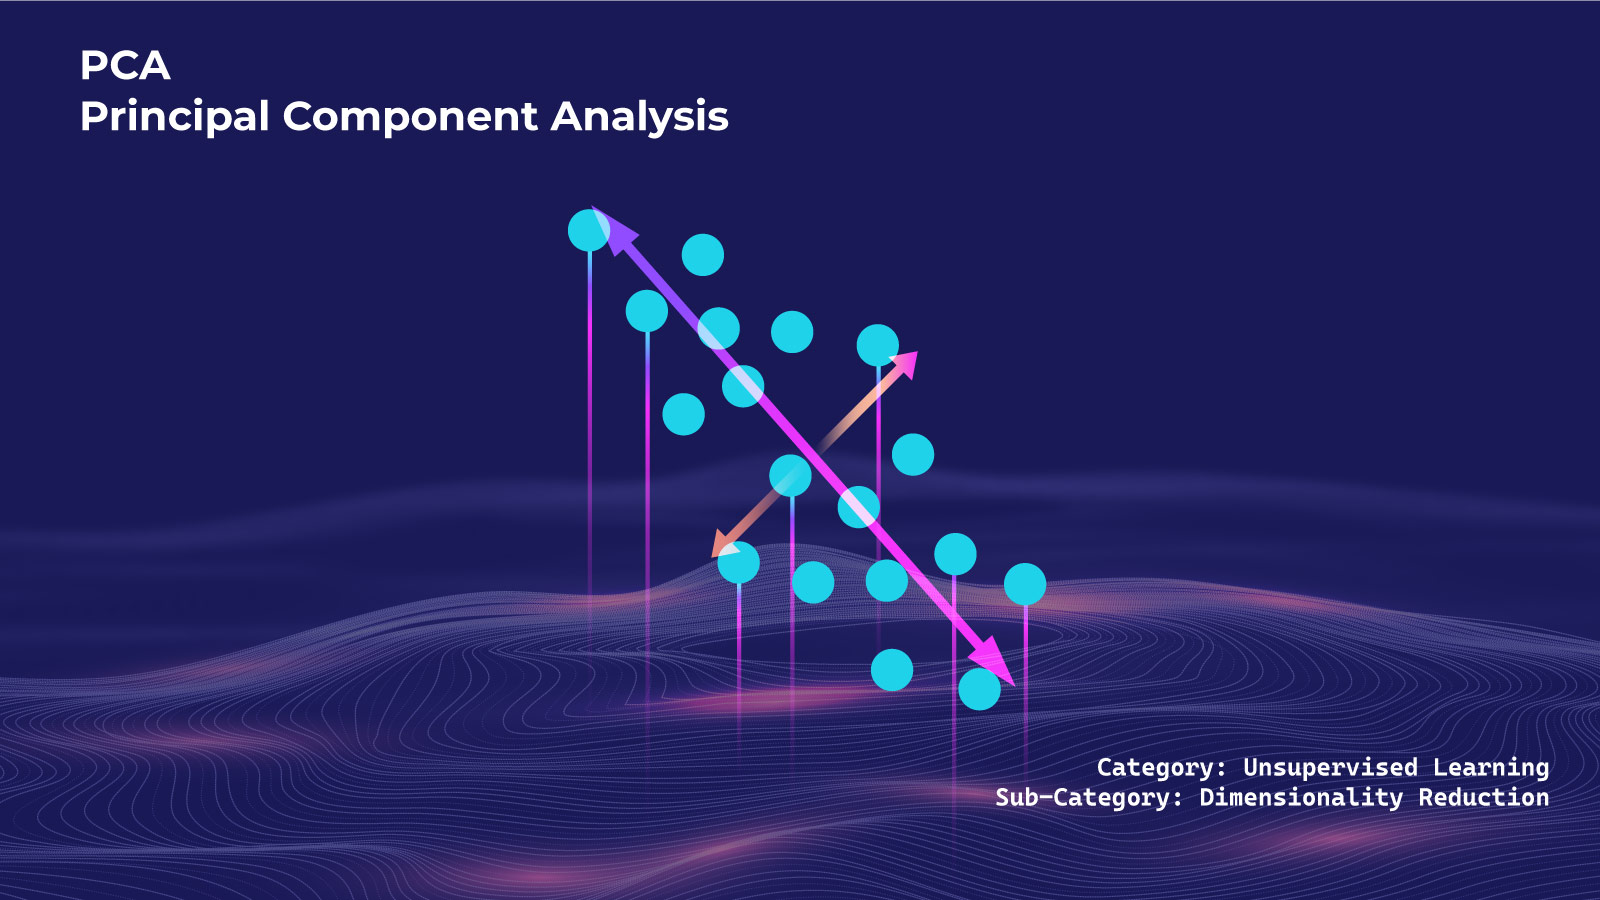
\includegraphics{images/01-Preface.jpg}}

}

\end{figure}

In recent times, the utilization of large datasets has become widespread
across numerous fields. To confront the challenges posed by these
complex datasets with multiple variables, unsupervised learning
algorithms, particularly Principal Component Analysis (PCA), assume a
crucial role in various tasks such as dimensionality reduction, feature
extraction, and data visualization. The roots of PCA can be traced back
to Karl Pearson's conceptualization in 1901, with subsequent
formalization by Harold Hotelling in 1933. PCA's primary objective is to
reduce data dimensionality while preserving its inherent variability. It
achieves this by generating principal components, which serve as
representatives for variables, thereby simplifying data representation
and enhancing exploratory data analysis. The underlying mathematical
framework of PCA revolves around identifying eigenvectors and
eigenvalues of the covariance matrix. With the development of software
packages, PCA has become easily accessible for data analysis. However,
PCA is most effective when data patterns result in statistical variance
that can be captured by the principal components, making it a potent
tool for data exploration but less suitable for non-linear or
non-orthogonal data. Careful consideration must be given to proper data
scaling. PCA finds application in diverse fields such as archaeology,
neuroscience, and the arts, enabling practitioners to explore datasets,
preprocess data, and streamline analysis. Moreover, it has found utility
in computer vision for tasks like facial recognition, showcasing its
prowess in reducing dimensionality while preserving crucial information.
Overall, PCA is a versatile and widely used technique in statistics and
data analysis, providing a valuable means to extract insights from
complex datasets and simplify decision-making processes across diverse
domains.

\bookmarksetup{startatroot}

\hypertarget{intro}{%
\chapter{Introduction}\label{intro}}

In recent years, the exponential growth of large datasets with numerous
variables have become increasingly prevalent across various fields
{[}1{]}, including but not limited to data analysis, image processing,
genetics, finance, and signal processing {[}2{]}. Analyzing, processing,
and visualizing these multivariate datasets pose significant challenges.
Therefore, the significance of unsupervised learning algorithms comes
into play, particularly in tasks like dimensionality reduction, feature
extraction, and visualization of complex data sets. Unsupervised
learning is a collection of algorithms to classify raw data {[}3{]}.
Clustering, and density estimation methods, often serve as a crucial
preliminary step in dimensionality reduction where the objective is to
find patterns and correlations aiding in organizing the original data.
The underlying structures and relationships within the data can inform
the selection and application of dimensionality reduction techniques.

Moreover, dimensionality reduction (DR) techniques aim to mitigate the
challenge of extracting valuable insights from complex data by reducing
the number of dimensions, decreasing computational complexity,
eliminating irrelevant and redundant data, improving algorithm accuracy,
and facilitating efficient data visualization {[}4{]}. Unsupervised
learning and dimensionality reduction are indispensable tools in data
analysis, and machine learning. While unsupervised learning aims to
uncover patterns and correlations between raw data, dimensionality
reduction simplifies data representation. One widely used DR technique
is Principal Component Analysis (PCA). The objectives of the present
research project are the comprehensive exploration of PCA, encompassing
an introduction to its core concepts, a discussion of its purposes and
functions as well as a demonstration of its application through
step-by-step examples.

Principal Component Analysis is best described as a dimension reduction
technique for statistical data. PCA has its roots in the work of Karl
Pearson in his 1901 paper ``On Lines and Planes of Closest Fit to
Systems of Points in Space'' {[}5{]} with the later christening and
formal development of the technique by Harold Hotelling in 1933 {[}6{]}.
Pearson initially conceptualized PCA as a geometric interpretation
within statistics; subsequently, PCA gained recognition as a more
suitable method than analysis of variance for modeling response data
{[}7{]}. The aim of PCA is to reduce the dimensionality of a dataset
without loss of information about the variability of the data. By
creating principal components that act as analogues for variables, the
statistical information of the dataset can be preserved and compressed
into a more easily representable form. A common example of the
application of PCA involves reducing an n-dimensional data set into 2
principal components which can be plotted on a graph representing the
relationships among the original variables; for this reason, PCA is
often described as an exploratory data analysis tool.

\hypertarget{theoretical-and-mathematical-foundations}{%
\section{Theoretical and mathematical
foundations}\label{theoretical-and-mathematical-foundations}}

The fundamental concept behind PCA is to explain the variability in a
set of correlated variables with a smaller set of uncorrelated
variables, thus mitigating issues such as multicollinearity. The
geometric properties of PCs facilitate an intuitive interpretation of
key features within complex multivariate datasets {[}8{]}; the first
principal component represents the direction with the greatest variation
in the original data, while subsequent components are uncorrelated with
the previous ones. Each component can be interpreted as the direction
that maximizes the variance of the original data when projecting new
observations onto the components {[}1{]}. PCA aims to capture a
significant proportion of the original variables' variation in the first
few components, offering a practical lower-dimensional summary. While
other methods may involve weighted averages across related variables to
reduce dimensions, PCA often achieves similar results with minimal loss
of variance information {[}9{]}. The mathematical foundations of PCA
center around data of \(p\) variables in \(n\) observations, represented
by an \(n \times p\) matrix \(X\) with the goal of finding a linear
combination of the columns of \(X\) which maximize variance. By
maximizing the variance in these linear combinations, we can capture the
largest amount of statistical information possible among the dimensions
of the dataset. As described by Jolliffe and Cadima {[}2{]}, this boils
down to finding the eigenvectors (\(a\)) and the largest eigenvalues
(\(\lambda\)) of the covariance matrix \(S\), where \(Xa_k\) are the
linear combinations called the principal components.

With the development of software packages in computer languages such as
R and Python, the computational burden of PCA for large datasets can be
easily handled by software; PCA has become easy to use as part of any
data processing pipeline. Abdi and Williams describe PCA as ``probably
the most popular multivariate statistical technique \ldots{} used by
almost all scientific disciplines.'' {[}10{]} Abdi and Williams also
emphasize that the goals of PCA should be extracting only the most
important information from a dataset to both compress and simplify the
dataset and provide a way to analyze the structure of the observations
and variables more easily. Importantly, the authors also offer a
geometric description of the principal components as orthogonal factors
to the original axis of the dataset; another strength of PCA is the fact
that the technique can be explained and expressed through several
mathematical avenues. Finally, Abdi and Williams offer methods to
evaluate the quality of the ``PCA model'' in reconstructing the original
data matrix using the derived principal components. For example,
calculating the residual sum of squares, or RESS, after rebuilding X
provides a way to identify model accuracy by seeking a minimal RESS
value from X and X.~

Lever and Altman {[}11{]} offer similar praises of PCA while echoing the
cautions of prior authors as a powerful data exploration tool with clear
limitations. PCA is best when interesting patterns in data produce
statistical variance which can be capture by the principal components,
but the technique is far less effective when patterns in data are
non-linear or non-orthogonal or when the maximization of variance fails
to produce interesting clusters in the principal component space.
Scaling is often necessary for PCA to ensure compatibility across
variables with different scales and ranges. The original data is
typically standardized to have a mean of 0 and a variance of 1 {[}8{]}.
PCA can be used improperly to produce results that obfuscate the actual
statistical content of the dataset; scaling may influence the analysis
with prior knowledge of the data, so the decision to scale the data and
the scaling methodology should be considered carefully.

\hypertarget{applications-and-extensions}{%
\section{Applications and
extensions}\label{applications-and-extensions}}

\hypertarget{in-archeology-neuroscience-and-the-arts}{%
\subsection{In Archeology, Neuroscience, and the
Arts}\label{in-archeology-neuroscience-and-the-arts}}

PCA has been utilized by many authors across numerous fields as an
essential part of a data analysis pipeline. As an example of the
application of PCA, Jolliffe and Cadima {[}2{]} present a dataset of 88
observations with 9 variables of measurement for fossilized mammal teeth
including length in two dimensions, width in two dimensions, and more.
With the R statistical language, finding and displaying the principal
components of the dataset becomes trivial work where patterns can be
identified graphically in a two-dimensional (PC1 x PC2) plot, versus the
original scatterplot which would be displayed in nine-dimensional space.
The development of statistical software has made it straightforward for
practitioners to use PCA for data exploration and dimensionality
reduction. Authors such as Maindonald and Braun {[}12{]} have produced
publications which present techniques and step-by-step methodologies of
using R to calculate principal components and graphically display the
results. Their presentation includes code snippets which can be run in R
software environments along with worked examples and a discussion of
results, facilitating the use of the technique for practitioners of all
experience levels.

Felipe Gewers and their research team directly expound on Abdi and
Williams' description of PCA as ``the most popular multivariate
statistical technique {[}...{]}'' in an analysis of publications which
use PCA: Across twenty-three disciplines ranging from Neuroscience to
the Arts, PCA is used to explore a dataset before analysis, used as part
of a spectrum of statistical analysis tools prior to modeling and
analysis, or used to preprocess and simplify data for direct analysis
and modeling {[}13{]}. The authors also discuss the broad effectiveness
of PCA in representing more than 50\% of the variance in most datasets
using only the first three principal components. They also highlight how
differences in captured variance appear between standardization and
non-standardization, and in different fields of study; PCA can be
effective in an incredibly diverse array of data when applied
appropriately. As an exploratory technique with a long tenure in the
field of statistics and data analysis, PCA is tried and true in
simplifying datasets and allowing practitioners to identify and explore
the largest sources of statistical information present in their data.

Principal Component Analysis is also implemented in Scikit Learn with
randomized Singular Value Decomposition (SVD) for dimensionality
reduction in data analysis, particularly for face recognition and
similar high-dimensional data applications. For instance, with an image
of 4096 dimensions (64x64 pixel gray scale images) PCA can transform the
data into a lower 200 dimension format that still captures the essential
information {[}14{]}. With randomized SVD it becomes computationally
more efficient to approximate the singular vectors, which are then used
to perform the transformation. This approach significantly reduces
computation time and memory usage. Additionally, PCA decomposes a
multivariate dataset into orthogonal components that explain the maximum
amount of variance. It can center and optionally scale the input data
before applying SVD. Scaling can be useful for downstream models, such
as Support Vector Machines with the RBF kernel and K-Means clustering,
which assume certain properties of the data distribution.

\hypertarget{computer-vision-and-pattern-recognition}{%
\subsection{Computer Vision and Pattern
Recognition}\label{computer-vision-and-pattern-recognition}}

The Eigenfaces concept has emerged as a groundbreaking approach to
facial detection and recognition. The Eigenfaces algorithm employs PCA
to extract essential facial features, reducing the dimensionality of
face images while retaining crucial information. The Eigenfaces
technique represents facial images in high-dimensional space while
projecting the images onto a lower-dimensional space. Turk and Pentland
demonstrated the effectiveness of Eigenfaces in recognizing faces under
various conditions, including variations in lighting, facial
expressions, and pose {[}15{]}. The potential implications of this
research extend beyond face recognition, and have broader implications
for image analysis, computer vision, and biometric systems. The paper
Eigenfaces by Zhang and Turk provided an insightful exploration of the
Eigenfaces method {[}16{]}, considered as the first working technique in
facial recognition. Eigenfaces leverage the power of PCA to represent
facial images compactly and efficiently, making it possible to recognize
faces in various contexts.

The idea of principal components to represent human faces was developed
by Sirovich and Kirby in 1987 and used by Turk and Pentland in 1991
{[}15{]} for face detection and recognition. The authors describe the
mathematical principles behind PCA, and its adaptation for facial
recognition, capturing the most prominent facial features while reducing
the dimensionality of the data. Specifically, the eigenfaces are the
principal components of a distribution of faces, or the eigenvectors of
the covariance matrix of the set of face images, where an image with N
pixels is considered a point (or vector) in N-dimensional space.
Emphasis is placed on the versatility of Eigenfaces in handling
variations in lighting, pose, and facial expressions, making it a robust
tool for real-world applications.

This application of PCA represents one of many for a longstanding
technique in the rapidly growing field of statistics and data analysis.
The unsupervised learning algorithm plays a vital role in dimensionality
reduction, feature extraction, and visualization of complex data sets.
Understanding PCA is crucial for researchers, and students seeking to
extract meaningful insights and patterns from high-dimensional data to
simplify the decision-making process.

\bookmarksetup{startatroot}

\hypertarget{methods}{%
\chapter{Methods}\label{methods}}

The aim of Principal component analysis (PCA) is to reduce the
dimensionality of multivariate data while preserving the variability
present in the data. The principal components derived from the dataset
are orthogonal variables represented by linear combinations of the
original variables which maximize variance. The first principal
component (PC) captures the most variance, followed by the second
orthogonal principal component, and so on. There can be as many PCs as
there are variables in the original data, but the technique is typically
used to simplify high-dimension data for improved interpretability.
Principal components can be calculated using eigenvalue decomposition or
the singular value decomposition (SVD) of the data matrix, so data must
be preproccesed and several assumptions met for PCA to yield meaningful
results.

\hypertarget{assumptions}{%
\section{Assumptions}\label{assumptions}}

For PCA to be effective, the data should be continuous (although
adaptations of PCA exist for other numeric data structures) and normally
distributed, although the the distribution of the data does not truly
matter when utilizing PCA as an exploratory methodology. More
importantly, the data should be linearly related or the linear
combinations of the principal components cannot meaningfully capture the
variance of the data. Ideally, the variables should be similar in scale,
and free from extreme outliers, or missing values, although this can be
addressed in preprocessing, and implementations of PCA such as robust
PCA have been developed to address these challenges. {[}2{]}

\hypertarget{preprocessing}{%
\section{Preprocessing}\label{preprocessing}}

Preprocessing data for PCA is straightforward. Missing data should be
handled using a method appropriate for the dataset, such as imputation
based on the mean or median of the variable observations. After this the
variables should be centered and scaled, to a mean of 0 and a standard
deviation of 1, although statistical software libraries for SVD and PCA
may include this as an option within the function. {[}17{]}

\hypertarget{eigenvectors}{%
\section{Eigenvectors}\label{eigenvectors}}

PCA uses eigenvectors and their corresponding eigenvalues to calculate
the principal components; a brief overview is given here. Eigen is a
German word meaning \emph{inherent} or \emph{characteristic}, and an
eigenvector can be described geometrically as a nonzero vector \(a\) of
a linear transformation matrix \(M\) which does not change direction
when the transformation is applied; the only change that occurs is a
scaling by factor \(\lambda\), the eigenvalue of the eigenvector \(a\).
Such a characteristic vector is useful in PCA, where the goal is to
maximize variance while reducing dimensionality, and in this context the
eigenvectors and eigenvalues can be thought of as the inherent
components of the dataset which contain the most important information.
Eigenvalues can be calculated from the characteristic polynomial of the
matrix, by taking the determinant of \(M - \lambda I\), where \(I\) is
the identity matrix. Setting this expression equal to zero allows the
calculation of the eigenvalues as the roots of the characteristic
polynomial; the resulting equation is called the characteristic
equation:

\begin{equation}\protect\hypertarget{eq-1}{}{
det(M - \lambda I) = 0
}\label{eq-1}\end{equation}

An eigenvalue \(\lambda_k\) can be used to solve for some eigenvector
\(a_k\) with the equation \((M - \lambda I)a = 0\). With PCA, we can use
the eigenvectors of the covariance matrix to compute the PCs. {[}18{]}

\hypertarget{principal-component-analysis}{%
\section{Principal Component
Analysis}\label{principal-component-analysis}}

In this approach to PCA, SVD is used to extract the most information
(variance) from the data matrix while reducing the dimensionality of the
data. The first principal component will have the largest possible
variance (also called inertia), whose value is defined as a factor
score. Factor scores represent a geometric projection of the
observations onto the PCs. The second PC, orthogonal to the first, has
the second largest variance, and the third PC would continue this
pattern. The calculation of PCs via SVD can be understood with the use
of matrix operations on a dataset. {[}19{]}

\hypertarget{centering-and-scaling}{%
\subsection{Centering and Scaling}\label{centering-and-scaling}}

Let our dataset be represented by the \(N \times P\) matrix \(X\)
comprised of \(N\) observations of \(P\) variables in the data set,
where any element \(x_{np}\) represents the \(n\)th observation of
variable \(p\) in the dataset. The matrix \(X\) has rank \(A\) where
\(A \leq min\{N, P\}\). The data in \(X\) is centered and scaled, such
that the mean of each column \(X_p\) is 0 and every \(x_{np}\) has been
standardized with scaled unit variance. We can represent this with the
formula:

\begin{equation}\protect\hypertarget{eq-2}{}{
z_{np} = \frac{x_{np} - \bar{x}_{p}}{{\sigma_{p}}}
}\label{eq-2}\end{equation}

\hypertarget{eigendecomposition-of-the-covariance-matrix}{%
\subsection{Eigendecomposition of the Covariance
Matrix}\label{eigendecomposition-of-the-covariance-matrix}}

The aim of PCA is to find some linear combination of the columns of
\(X\) which maximizes the variance. If we define \(a\) as a vector of
constants \(a_1, a_2, a_3, …, a_p\), then \(Xa\) represents the linear
combination of interest. The variance of \(Xa\) is represented by
\(var(Xa) = a^TSa\), with the covariance matrix \(S\), and \(T\)
representing the transpose operator. Finding the \(Xa\) with maximum
variance equates to finding the vector \(a\) which maximizes the
quadratic \(a^TSa\), where \(a^Ta = 1\). We can write this as
\(a^TSa - \lambda(a^Ta-1)\), with the Lagrange multiplier \(\lambda\).
{[}20{]} Equating this expression to the null vector \(0\) allows us to
differentiate with respect to \(a\):

\begin{equation}\protect\hypertarget{eq-3}{}{
Sa - \lambda a = 0 \Rightarrow Sa = \lambda a
}\label{eq-3}\end{equation}

Therefore, \(a\) is a unit-norm eigenvector with eigenvalue \(\lambda\)
of the covariance matrix \(S\). The largest eigenvalue of \(S\) is
\(\lambda_1\) with the eigenvector \(a_1\), which we can define for any
eigenvector \(a\):

\begin{equation}\protect\hypertarget{eq-4}{}{
var(Xa) = a^TSa = \lambda a^Ta = \lambda
}\label{eq-4}\end{equation}

Any \(p \times p\) real symmetric matrix has exactly \(p\) real
eigenvalues \(\lambda_k\) for \(k = 1,...,p\). The corresponding
eigenvectors of these eigenvalues can be defined to form an orthonormal
set of vectors such that \(a_k^Ta_{k^T} = 1\) if \(k = k^T\) and zero
otherwise. If we consider that \(S\) is such a matrix and impose the
restriction of orthogonality to the different coefficient vectors of
\(S\), the full set of eigenvectors of \(S\) represent the solutions to
finding linear combinations \(Xa_k\) which maximize variance while
minimizing correlation with prior linear combinations. \(Xa_k\) then
represent the linear combinations which are the principal components of
the dataset with eigenvectors \(a_k\) and eigenvalues \(\lambda_k\). The
elements of \(Xa_k\) are the factor scores of the PCs, while the
elements of the eigenvectors \(a_k\) represent the loadings of the PCs.
{[}2{]}

\hypertarget{singular-value-decomposition}{%
\subsection{Singular Value
Decomposition}\label{singular-value-decomposition}}

Next we define the singular value decomposition of \(X\). Let \(L\) be
the \(N \times A\) matrix of left singular vectors of the matrix; that
is, the columns of \(L\) are made up of the eigenvectors of \(XX^T\).
Let \(R\) be the \(P \times A\) matrix of right singular vectors; the
columns of \(R\) are made up of the eigenvectors of \(X^TX\). Finally,
let \(D\) be the diagonal matrix of singular values, meaning the
singular values in \(D\) are the square roots of the eigenvalues of
\(XX^T\) and \(X^TX\), and \(D^2\) is defined as the diagonal matrix of
the non-zero eigenvalues. We can define the singular value decomposition
of matrix \(X\) as:

\begin{equation}\protect\hypertarget{eq-5}{}{
X = LD{R}^T
}\label{eq-5}\end{equation}

In this context, the eigenvalues represent the variances of the
principal components and summarily contain the important information for
the dataset, and we can obtain the PCs of \(X\) from the SVD. {[}10{]}
With the identity matrix \(I\), the \(I \times R\) matrix of factor
scores can be expressed as:

\begin{equation}\protect\hypertarget{eq-6}{}{
F = LD
}\label{eq-6}\end{equation}

These factor scores are calculated from the coefficients of the linear
combinations in matrix \(R\), which can be defined as a projection
matrix of the original observations onto the PCs, i.e.~the product of
\(X\) and \(R\):

\begin{equation}\protect\hypertarget{eq-7}{}{
F = LD = LDR^TR = XR
}\label{eq-7}\end{equation}

The matrix \(R\) is also referred to as a loading matrix, and \(X\) is
often described as the product of the factor score matrix and the
loading matrix:

\begin{equation}\protect\hypertarget{eq-8}{}{
X = FR^T
}\label{eq-8}\end{equation}

with the decomposition of \(F^TF = D^2\) and \(R^TR = I\).

The loadings represent the weights of the original variables in the
computation of the PCs; in other words, the correlation from -1 to 1 of
each variable with the factor score.

In a geometric interpretation of PCA, the factor scores measure length
on the Cartesian plane. This length represents the projection of the
original observations onto the PCs from the origin at \((0, 0)\). This
is especially useful as a visualization of higher dimension data in two
dimensions by utilizing the first two PCs which capture the most
variance in the original data. {[}11{]}

\hypertarget{interpretation-of-the-principal-components}{%
\section{Interpretation of the Principal
Components}\label{interpretation-of-the-principal-components}}

There are several ways to interpret the PCs derived from the analysis.
Since the eigenvalues represent the variance of the PCs, the proportion
of the eigenvalues explain the proportion of variation in the dataset.
Using a scree plot, these eigenvalues are plotted to show how much
variation each PC explains. Another commonly used tool is a biplot, a
combination of the plots of the factor scores (points) and the loadings
(vectors) for two PCs (typically PC1 and PC2). The biplot is meant to
visually capture the relationship between the original variables and the
principal components. Clusters of points represent highly correlated
variables, and vector lengths represent the variability captured in that
direction on the principal component axis. While many methods and tools
exist to interpret the results of PCA, the usefulness of each depends on
the needs of the analysis. {[}18{]}

\bookmarksetup{startatroot}

\hypertarget{examples}{%
\chapter{Examples}\label{examples}}

Moving beyond the theoretical foundations of principal components, how
is PCA applied to data? We offer two examples; the first a demonstration
of the manual calculation of principal components, and the second
implementing PCA on a large dataset using R.

\hypertarget{manual-calculation-of-principal-components}{%
\section{Manual calculation of principal
components}\label{manual-calculation-of-principal-components}}

In this illustration, we have access to the two grades of four students
in a statistics subject. We aim to employ principal component analysis
as a means to reduce the dimensionality from two variables to a singular
variable. This transformation will effectively represent students'
performance in the subject with a more compact and interpretable
measure. This example is adapted from the resource \emph{How to compute
principal components} {[}21{]}.

\begin{longtable}[]{@{}lll@{}}
\toprule\noalign{}
Scores & \textbf{Basic Stats} & \textbf{Advanced Stats} \\
\midrule\noalign{}
\endhead
\bottomrule\noalign{}
\endlastfoot
\textbf{Student 1} & \textbf{4} & \textbf{11} \\
\textbf{Student 2} & \textbf{8} & \textbf{4} \\
\textbf{Student 3} & \textbf{13} & \textbf{5} \\
\textbf{Student 4} & \textbf{7} & \textbf{14} \\
\textbf{Mean} & \(\bar{x}\) = \textbf{8} & \(\bar{y}\) = \textbf{8.5} \\
\end{longtable}

\hypertarget{calculate-the-covariance-matrix-m}{%
\subsection{\texorpdfstring{Calculate the covariance matrix
\(M\)}{Calculate the covariance matrix M}}\label{calculate-the-covariance-matrix-m}}

\[
\begin{bmatrix}
\text{cov}(x,x) & \text{cov}(x,y) \\
\text{cov}(y,x) & \text{cov}(y,y) \\
\end{bmatrix}
\]

\(\Rightarrow\) \(\text{cov}(x,x)\) = \(\text{var}(x)\) =
\(\mathbf{E}\)(\(x^2\)) - \(\mathbf{E}\) \((x)^2\) =
\[ \frac{(16+0+25+1)}{3}=14 \]

\(\Rightarrow\) \(\text{cov}(y,y)\) = \(\text{var}(y)\) =
\(\mathbf{E}\)(\(y^2\)) - \(\mathbf{E}\) \((y)^2\) =
\[ \frac{(6.25+20.25+12.25+30.25)}{3}=23 \]

\(\Rightarrow\) \(\text{cov}(x,y)\) = \(\text{cov}(y,x)\) =
\(\mathbf{E}\)(\(xy\)) - \(\mathbf{E}\) (\(x\))\(\mathbf{E}\) (\(y\)) =
\[ \frac{(-10+0-17.5-5.5)}{3}=-11 \]

\(\Rightarrow\) Covariance Matrix \(M\) \[ 
\begin{bmatrix}
14 & -11 \\
-11 & 23 \\
\end{bmatrix} \]

\hypertarget{compute-the-singular-value-decomposition-svd}{%
\subsection{Compute the singular value decomposition
(SVD)}\label{compute-the-singular-value-decomposition-svd}}

We can obtain the principal components and loadings from SVD of the
covariance matrix M since covariance matrix M is a square matrix:

\[ 
\begin{bmatrix}
14 & -11 \\
-11 & 23 \\
\end{bmatrix} \times Any\ vector = \lambda \times Any\ vector\ ,\ (vector\neq 0) 
\]

\[det(M - \lambda I) = 0\]

\hypertarget{obtain-eigenvalues-of-the-covariance-matrix-rightarrow-lambda_1-lambda_2}{%
\subsubsection{\texorpdfstring{Obtain eigenvalues of the covariance
matrix \(\rightarrow\) \(\lambda_1\) \&
\(\lambda_2\)}{Obtain eigenvalues of the covariance matrix \textbackslash rightarrow \textbackslash lambda\_1 \& \textbackslash lambda\_2}}\label{obtain-eigenvalues-of-the-covariance-matrix-rightarrow-lambda_1-lambda_2}}

\[
I = \begin{bmatrix}
1 & 0 \\
0 & 1 \\
\end{bmatrix}
\]

\[
\lambda I = \lambda \times \begin{bmatrix}
1 & 0 \\
0 & 1 \\
\end{bmatrix} = \begin{bmatrix} 
\lambda  & 0 \\
0 & \lambda  \\
\end{bmatrix}
\]

\[
\begin{bmatrix}
14 & -11 \\
-11&  23 \\
\end{bmatrix} -\begin{bmatrix}
\lambda  & 0 \\
0 & \lambda  \\
\end{bmatrix} = \begin{bmatrix}
14-\lambda  & -11 \\
-11 & 23-\lambda  \\
\end{bmatrix}
\]

\(\Rightarrow\)

\[
det\begin{bmatrix}
 14-\lambda & -11 \\
 -11& 23-\lambda  \\
\end{bmatrix}=0
\]

\(\Rightarrow\) \[(14-\lambda)(23-\lambda) - (-11)(-11) = 0 \]

\[\lambda^2 +37\lambda -201 = 0\]

\(\Rightarrow\) \(\lambda_1\) = 30.3849, \(\lambda_2\) = 6.6152
(eigenvalues for Covariance Matrix \(M\))

\hypertarget{obtain-eigenvector-of-lambda_1}{%
\subsubsection{\texorpdfstring{Obtain eigenvector of
\(\lambda_1\)}{Obtain eigenvector of \textbackslash lambda\_1}}\label{obtain-eigenvector-of-lambda_1}}

\[(M - \lambda_1I)\times U_1 = \mathbf{0} \]

\(\Rightarrow\) \[\begin{bmatrix}
 14-\lambda & -11 \\
 -11& 23-\lambda  \\
\end{bmatrix}\times\begin{bmatrix}
u_1 \\
u_2 \\
\end{bmatrix}=\mathbf{0}
\]

\[(14- \lambda)u_1 - 11u_2 = 0 \] \(\Rightarrow\)
\[-16.3849u_1 -11u_2 = 0\] \(\Rightarrow\) \[-16.3849u_1= 11u_2 \]
\(\Rightarrow\) \[u_1 = \frac{11}{-16.3849}u_2\]

\[
\begin{bmatrix}
u_1 \\
u_2 \\
\end{bmatrix}= u_2\begin{bmatrix}
\frac{11}{-16.3849}\\
1 \\
\end{bmatrix}
\]

\(\Rightarrow\) \[u_2\begin{bmatrix}
-11\\ 16.3849
\end{bmatrix}\]

\[
\begin{bmatrix}
16.3849 & 11 \\
\end{bmatrix} \times \begin{bmatrix}
u_1 \\ u_2
\end{bmatrix} = \begin{bmatrix}
11 \\ -16.3849
\end{bmatrix}
\]

\textbf{Normalized Eigenvector}

\(\Rightarrow\) \(\lambda_1\): \(e_1\)

\[
\frac{1}{\sqrt{{11^2 +16.3849^2}}}\begin{bmatrix}
11 \\ -16.3849
\end{bmatrix}= \begin{bmatrix}
0.5574 \\ -0.8303
\end{bmatrix} 
\]

\(\Rightarrow\) \(\lambda_2\) \(e_2\) (Right singular vector) =

\[
\begin{bmatrix}
0.8303 \\ 0.5574
\end{bmatrix} 
\]

\hypertarget{derive-the-new-dataset}{%
\subsection{Derive The new dataset}\label{derive-the-new-dataset}}

\textbf{First Principal Component (PC1)}

\[
P_{11} = e_1^T \times 
\begin{bmatrix}
4-mean(x) \\ 11 -mean(y)
\end{bmatrix}
 = \begin{bmatrix}
0.5574 & -0.8303 \\
\end{bmatrix} 
\begin{bmatrix}
4-8 \\ 11-8.5
\end{bmatrix} =-4.3052 
\]

\[
P_{12} = e_1^T \times 
\begin{bmatrix}
8-mean(x) \\ 4 -mean(y)
\end{bmatrix}
 = \begin{bmatrix}
0.5574 & -0.8303 \\
\end{bmatrix} 
\begin{bmatrix}
8-8 \\ 4-8.5
\end{bmatrix} =3.7361 
\]

\[
P_{13} = e_1^T \times 
\begin{bmatrix}
13-mean(x) \\ 5 -mean(y)
\end{bmatrix}
 = \begin{bmatrix}
0.5574 & -0.8303 \\
\end{bmatrix} 
\begin{bmatrix}
13-8 \\ 5-8.5
\end{bmatrix}= 5.6928
\]

\[
P_{14}= e_1^T \times 
\begin{bmatrix}
7-mean(x) \\ 14 -mean(y)
\end{bmatrix}
 = \begin{bmatrix}
0.5574 & -0.8303 \\
\end{bmatrix} 
\begin{bmatrix}
7-8 \\ 14-8.5
\end{bmatrix} = -5.1238
\]

\textbf{The new dataset (Left singular vector)}

\begin{longtable}[]{@{}
  >{\centering\arraybackslash}p{(\columnwidth - 8\tabcolsep) * \real{0.1304}}
  >{\centering\arraybackslash}p{(\columnwidth - 8\tabcolsep) * \real{0.2174}}
  >{\centering\arraybackslash}p{(\columnwidth - 8\tabcolsep) * \real{0.2174}}
  >{\centering\arraybackslash}p{(\columnwidth - 8\tabcolsep) * \real{0.2174}}
  >{\centering\arraybackslash}p{(\columnwidth - 8\tabcolsep) * \real{0.2174}}@{}}
\toprule\noalign{}
\begin{minipage}[b]{\linewidth}\centering
\end{minipage} & \begin{minipage}[b]{\linewidth}\centering
\textbf{Student 1}
\end{minipage} & \begin{minipage}[b]{\linewidth}\centering
\textbf{Student 2}
\end{minipage} & \begin{minipage}[b]{\linewidth}\centering
\textbf{Student 3}
\end{minipage} & \begin{minipage}[b]{\linewidth}\centering
\textbf{Student 4}
\end{minipage} \\
\midrule\noalign{}
\endhead
\bottomrule\noalign{}
\endlastfoot
\textbf{PC1} & \textbf{-4.3052} & \textbf{3.7361} & \textbf{5.6928} &
\textbf{-5.1238} \\
\end{longtable}

\hypertarget{verifying-and-visualizing-the-results}{%
\subsection{Verifying and visualizing the
results}\label{verifying-and-visualizing-the-results}}

\begin{table}

\caption{Dataframe structure}
\centering
\begin{tabular}[t]{l|l|l}
\hline
Student & BasicStats & AdvancedStats\\
\hline
1 & 4 & 11\\
\hline
2 & 8 & 4\\
\hline
3 & 13 & 5\\
\hline
4 & 7 & 14\\
\hline
\end{tabular}
\end{table}

\begin{table}

\caption{Importance of components}
\centering
\begin{tabular}[t]{l|l|l}
\hline
  & PC1 & PC2\\
\hline
Standard deviation & 1.270042 & 0.6220884\\
\hline
Proportion of Variance & 0.806500 & 0.1935000\\
\hline
Cumulative Proportion & 0.806500 & 1.0000000\\
\hline
\end{tabular}
\end{table}

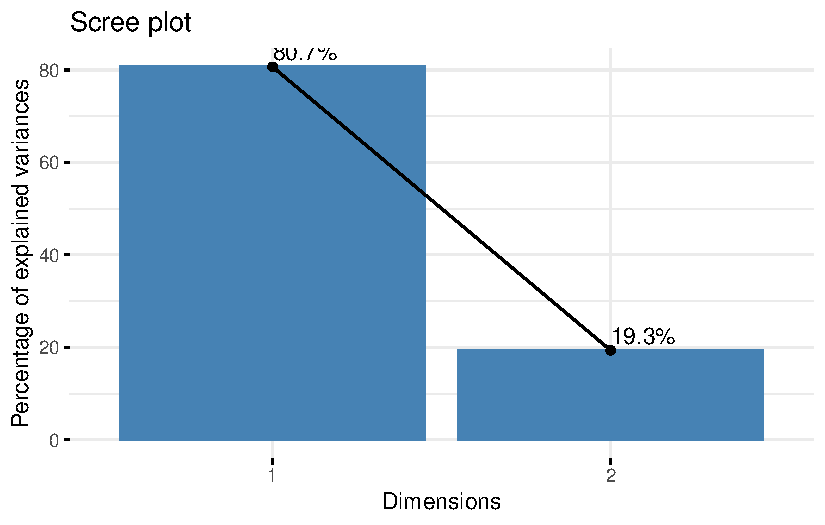
\includegraphics{examples_files/figure-pdf/unnamed-chunk-1-1.pdf}

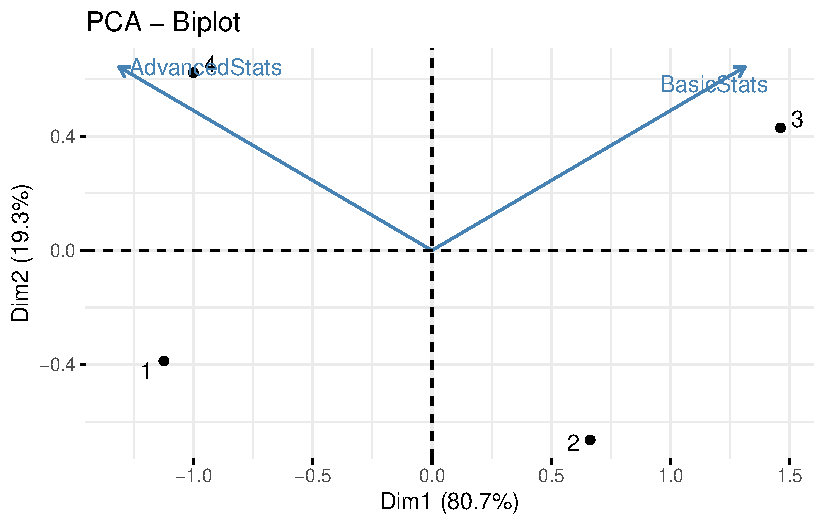
\includegraphics{examples_files/figure-pdf/unnamed-chunk-1-2.pdf}

\hypertarget{results}{%
\subsection{Results}\label{results}}

The first principal component of the data captures 80.7\% of the
variation (or information) while reducing the dimensionality of the
dataset from 2 variables to 1. Small datasets such as this make the
hand-calculation of principal components feasible and easy to follow,
but the strengths of PCA are especially evident when software is used to
enable principal component analysis for large datasets. In the next
example, we demonstrate how PCA can be used with a large dataset using
the R programming language.

\hypertarget{pca-on-a-large-dataset-using-r}{%
\section{PCA on a large dataset using
R}\label{pca-on-a-large-dataset-using-r}}

For this application of PCA, the Abalone dataset from the UCI Machine
Learning Repository is used {[}22{]}. This dataset contain 4177
observations of 9 variables which record characteristics of each abalone
including sex, length, diameter, height, weights, and the number of
rings. The variables, apart from sex, are continuous and correlated
making the dataset an ideal candidate for demonstrating dimensionality
reduction via PCA.

\hypertarget{libraries}{%
\subsection{Libraries}\label{libraries}}

First, the appropriate and necessary libraries are loaded in R. These
provide the functions which serve as the backbone of the analysis,
handling the computational aspects of PCA as well as visualizing the
results.

\begin{Shaded}
\begin{Highlighting}[]
\CommentTok{\# Load necessary libraries}
\FunctionTok{library}\NormalTok{(tidyverse)  }\CommentTok{\# for handling missing values}
\FunctionTok{library}\NormalTok{(corrplot) }\CommentTok{\# for plotting the correlation matrix}
\FunctionTok{library}\NormalTok{(factoextra) }\CommentTok{\# PCA plots}
\FunctionTok{library}\NormalTok{(summarytools) }\CommentTok{\#produces summary stats}
\end{Highlighting}
\end{Shaded}

\hypertarget{data-preparation}{%
\subsection{Data Preparation}\label{data-preparation}}

The dataset contains 9 variables with 1 categorical variable and 8
numeric variables. The dataset contains no missing values. For this
example in applying principal component analysis, we exclude the
categorical variable `Sex' and focus the PCA on the numerical dimensions
of the Abalone. For analyses involving a mix of numeric and non-numeric
variables other factor analysis techniques can be used, such as factor
analysis of mixed data {[}23{]}.

\begin{Shaded}
\begin{Highlighting}[]
\CommentTok{\# Load dataset}
\NormalTok{abalone }\OtherTok{\textless{}{-}} \FunctionTok{read.csv}\NormalTok{(}\StringTok{\textquotesingle{}./abalone/abalone.csv\textquotesingle{}}\NormalTok{)}

\NormalTok{data\_desc }\OtherTok{=} \FunctionTok{descr}\NormalTok{(abalone, }\AttributeTok{plain.ascii =} \ConstantTok{FALSE}\NormalTok{, }\AttributeTok{headings =} \ConstantTok{FALSE}\NormalTok{) }\CommentTok{\# descriptive statistics for the dataset}

\NormalTok{data\_desc }\SpecialCharTok{\%\textgreater{}\%}
  \FunctionTok{kbl}\NormalTok{(}\AttributeTok{align=} \StringTok{\textquotesingle{}l\textquotesingle{}}\NormalTok{) }\SpecialCharTok{\%\textgreater{}\%}
  \FunctionTok{kable\_paper}\NormalTok{(}\StringTok{"hover"}\NormalTok{)}
\end{Highlighting}
\end{Shaded}

\begin{table}
\centering
\begin{tabular}[t]{l|l|l|l|l|l|l|l|l}
\hline
  & Diameter & Height & Length & Rings & Shell\_weight & Shucked\_weight & Viscera\_weight & Whole\_weight\\
\hline
Mean & 0.4078813 & 0.1395164 & 0.5239921 & 9.9336845 & 0.2388309 & 0.3593675 & 0.1805936 & 0.8287422\\
\hline
Std.Dev & 0.0992399 & 0.0418271 & 0.1200929 & 3.2241690 & 0.1392027 & 0.2219629 & 0.1096143 & 0.4903890\\
\hline
Min & 0.0550000 & 0.0000000 & 0.0750000 & 1.0000000 & 0.0015000 & 0.0010000 & 0.0005000 & 0.0020000\\
\hline
Q1 & 0.3500000 & 0.1150000 & 0.4500000 & 8.0000000 & 0.1300000 & 0.1860000 & 0.0935000 & 0.4415000\\
\hline
Median & 0.4250000 & 0.1400000 & 0.5450000 & 9.0000000 & 0.2340000 & 0.3360000 & 0.1710000 & 0.7995000\\
\hline
Q3 & 0.4800000 & 0.1650000 & 0.6150000 & 11.0000000 & 0.3290000 & 0.5020000 & 0.2530000 & 1.1530000\\
\hline
Max & 0.6500000 & 1.1300000 & 0.8150000 & 29.0000000 & 1.0050000 & 1.4880000 & 0.7600000 & 2.8255000\\
\hline
MAD & 0.0963690 & 0.0370650 & 0.1186080 & 2.9652000 & 0.1475187 & 0.2349921 & 0.1178667 & 0.5285469\\
\hline
IQR & 0.1300000 & 0.0500000 & 0.1650000 & 3.0000000 & 0.1990000 & 0.3160000 & 0.1595000 & 0.7115000\\
\hline
CV & 0.2433058 & 0.2998003 & 0.2291884 & 0.3245693 & 0.5828504 & 0.6176489 & 0.6069664 & 0.5917269\\
\hline
Skewness & -0.6087607 & 3.1265706 & -0.6394138 & 1.1133019 & 0.6204809 & 0.7185815 & 0.5914271 & 0.5305773\\
\hline
SE.Skewness & 0.0378868 & 0.0378868 & 0.0378868 & 0.0378868 & 0.0378868 & 0.0378868 & 0.0378868 & 0.0378868\\
\hline
Kurtosis & -0.0482711 & 75.8953091 & 0.0616411 & 2.3239123 & 0.5281636 & 0.5912553 & 0.0809994 & -0.0264756\\
\hline
N.Valid & 4177.0000000 & 4177.0000000 & 4177.0000000 & 4177.0000000 & 4177.0000000 & 4177.0000000 & 4177.0000000 & 4177.0000000\\
\hline
Pct.Valid & 100.0000000 & 100.0000000 & 100.0000000 & 100.0000000 & 100.0000000 & 100.0000000 & 100.0000000 & 100.0000000\\
\hline
\end{tabular}
\end{table}

The summary statistics show the differences in measurement between
variables, with some variables such as diameter and viscera weight
having small ranges and others, namely rings, having relatively large
ranges. For this reason, scaling of the variables is a crucial step in
PCA to ensure results accurately capture the variance in the data.

\hypertarget{feature-scaling}{%
\subsection{Feature Scaling}\label{feature-scaling}}

Standardization ensures all variables, also called features, are on the
same scale, and the scale function allows us to center the data to a
mean of 0 and variance of 1. This ensures no single feature has an
outsized effect during the principal component analysis.

\begin{Shaded}
\begin{Highlighting}[]
\CommentTok{\# Select only the numeric variables }
\NormalTok{abalone }\OtherTok{=} \FunctionTok{select\_if}\NormalTok{(abalone, is.numeric)}

\CommentTok{\# Standardization of numerical features}
\NormalTok{abalone\_sc }\OtherTok{\textless{}{-}} \FunctionTok{scale}\NormalTok{(abalone, }\AttributeTok{center =} \ConstantTok{TRUE}\NormalTok{, }\AttributeTok{scale =} \ConstantTok{TRUE}\NormalTok{)}

\NormalTok{sc\_sum }\OtherTok{=} \FunctionTok{summary}\NormalTok{(abalone\_sc)}

\FunctionTok{kbl}\NormalTok{(sc\_sum, }\AttributeTok{align=} \StringTok{\textquotesingle{}l\textquotesingle{}}\NormalTok{) }\SpecialCharTok{\%\textgreater{}\%}
  \FunctionTok{kable\_paper}\NormalTok{(}\StringTok{"hover"}\NormalTok{)}
\end{Highlighting}
\end{Shaded}

\begin{table}
\centering
\begin{tabular}[t]{l|l|l|l|l|l|l|l|l}
\hline
  &     Length &    Diameter &     Height &  Whole\_weight & Shucked\_weight & Viscera\_weight &  Shell\_weight &     Rings\\
\hline
 & Min.   :-3.7387 & Min.   :-3.5558 & Min.   :-3.33555 & Min.   :-1.68589 & Min.   :-1.6145 & Min.   :-1.64298 & Min.   :-1.7049 & Min.   :-2.7708\\
\hline
 & 1st Qu.:-0.6161 & 1st Qu.:-0.5832 & 1st Qu.:-0.58614 & 1st Qu.:-0.78966 & 1st Qu.:-0.7811 & 1st Qu.:-0.79455 & 1st Qu.:-0.7818 & 1st Qu.:-0.5997\\
\hline
 & Median : 0.1749 & Median : 0.1725 & Median : 0.01156 & Median :-0.05963 & Median :-0.1053 & Median :-0.08752 & Median :-0.0347 & Median :-0.2896\\
\hline
 & Mean   : 0.0000 & Mean   : 0.0000 & Mean   : 0.00000 & Mean   : 0.00000 & Mean   : 0.0000 & Mean   : 0.00000 & Mean   : 0.0000 & Mean   : 0.0000\\
\hline
 & 3rd Qu.: 0.7578 & 3rd Qu.: 0.7267 & 3rd Qu.: 0.60926 & 3rd Qu.: 0.66123 & 3rd Qu.: 0.6426 & 3rd Qu.: 0.66056 & 3rd Qu.: 0.6478 & 3rd Qu.: 0.3307\\
\hline
 & Max.   : 2.4232 & Max.   : 2.4397 & Max.   :23.68045 & Max.   : 4.07178 & Max.   : 5.0848 & Max.   : 5.28587 & Max.   : 5.5040 & Max.   : 5.9136\\
\hline
\end{tabular}
\end{table}

Viewing the data after scaling and centering, values greater than 3 or
less than -3 represent outliers more than 3 standard deviations from the
mean. Based on the ranges of the variables, we should view a boxplot of
the data to further investigate.

\begin{Shaded}
\begin{Highlighting}[]
\CommentTok{\# Plot a boxplot to visualize potential outliers}
\FunctionTok{par}\NormalTok{(}\AttributeTok{mar=}\FunctionTok{c}\NormalTok{(}\DecValTok{4}\NormalTok{, }\DecValTok{8}\NormalTok{, }\DecValTok{4}\NormalTok{, }\DecValTok{4}\NormalTok{))}
\FunctionTok{boxplot}\NormalTok{(abalone\_sc, }\AttributeTok{col =} \StringTok{"steelblue"}\NormalTok{, }\AttributeTok{main =} \StringTok{"Visualization of scaled and centered data"}\NormalTok{, }\AttributeTok{horizontal =} \ConstantTok{TRUE}\NormalTok{, }\AttributeTok{las =} \DecValTok{1}\NormalTok{)}
\end{Highlighting}
\end{Shaded}

\begin{figure}[H]

{\centering 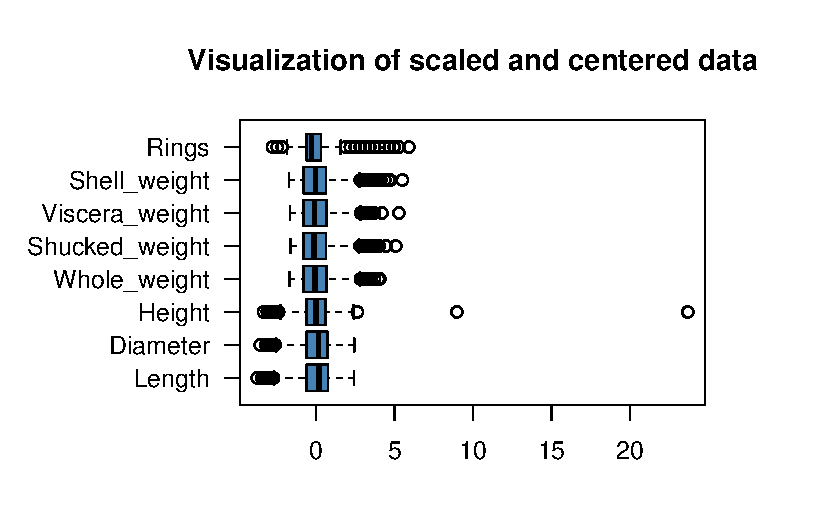
\includegraphics{examples_files/figure-pdf/unnamed-chunk-5-1.pdf}

}

\end{figure}

Are there enough outliers to be a cause for concern? We can see how many
lie outside of the third standard deviation of the data for each
variable.

\begin{Shaded}
\begin{Highlighting}[]
\NormalTok{outs }\OtherTok{=} \FunctionTok{colSums}\NormalTok{(abalone\_sc }\SpecialCharTok{\textgreater{}} \DecValTok{3} \SpecialCharTok{|}\NormalTok{ abalone\_sc }\SpecialCharTok{\textless{}} \SpecialCharTok{{-}}\DecValTok{3}\NormalTok{)}

\FunctionTok{kbl}\NormalTok{(outs, }\AttributeTok{col.names =}\NormalTok{ (}\StringTok{\textquotesingle{}Outliers\textquotesingle{}}\NormalTok{), }\AttributeTok{align =} \StringTok{\textquotesingle{}l\textquotesingle{}}\NormalTok{) }\SpecialCharTok{\%\textgreater{}\%}
  \FunctionTok{kable\_paper}\NormalTok{(}\StringTok{"hover"}\NormalTok{)}
\end{Highlighting}
\end{Shaded}

\begin{table}
\centering
\begin{tabular}[t]{l|l}
\hline
  & Outliers\\
\hline
Length & 15\\
\hline
Diameter & 13\\
\hline
Height & 5\\
\hline
Whole\_weight & 19\\
\hline
Shucked\_weight & 37\\
\hline
Viscera\_weight & 22\\
\hline
Shell\_weight & 27\\
\hline
Rings & 62\\
\hline
\end{tabular}
\end{table}

Of the 4177 observations, at most 62 in a single variable (Rings) are
outliers. The tolerance for outliers will differ depending on the
investigation, but for our illustrative purposes this number is well
within tolerance for principal component analysis.

Lastly, we can investigate the correlation among the variables. PCA is
best used with linearly correlated data. If the data is not correlated,
the results of PCA will be less meaningful.

\begin{Shaded}
\begin{Highlighting}[]
\CommentTok{\# Calculate correlations and round to 2 digits}
\NormalTok{abalone\_corr }\OtherTok{\textless{}{-}} \FunctionTok{cor}\NormalTok{(abalone\_sc)}
\FunctionTok{corrplot}\NormalTok{(abalone\_corr, }\AttributeTok{method=}\StringTok{"number"}\NormalTok{)}
\end{Highlighting}
\end{Shaded}

\begin{figure}[H]

{\centering 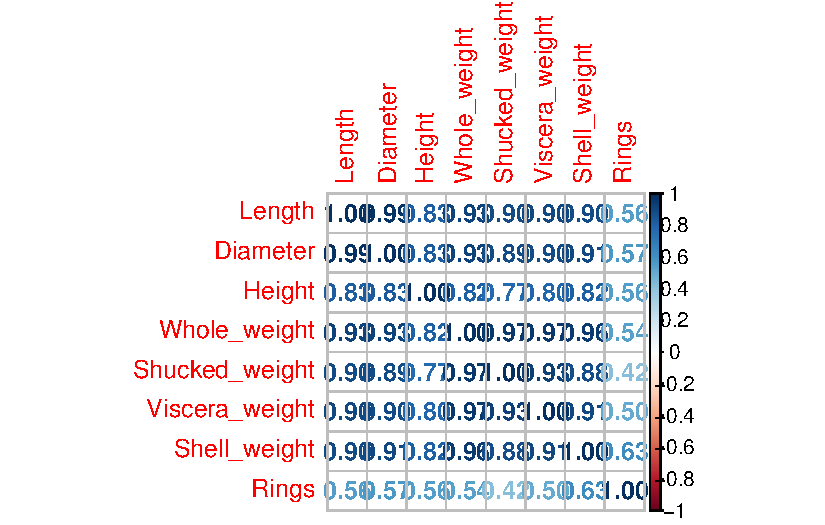
\includegraphics{examples_files/figure-pdf/unnamed-chunk-7-1.pdf}

}

\end{figure}

Our scaled and centered data has strong linear correlations and contains
a relatively small number of outliers. We can now calculate the
principal components of the dataset.

\hypertarget{pca-via-singular-value-decomposition}{%
\subsection{PCA via Singular Value
Decomposition}\label{pca-via-singular-value-decomposition}}

The prcomp() function {[}17{]} performs principal component analysis on
a dataset using the singular value decomposition method, which utilizes
the covariance matrix of the data.

\begin{Shaded}
\begin{Highlighting}[]
\CommentTok{\# Apply PCA using prcomp()}
\NormalTok{abalone\_pca }\OtherTok{\textless{}{-}} \FunctionTok{prcomp}\NormalTok{(abalone\_sc)}

\NormalTok{sum\_pca }\OtherTok{=} \FunctionTok{as.data.frame}\NormalTok{(}\FunctionTok{summary}\NormalTok{(abalone\_pca)}\SpecialCharTok{$}\NormalTok{importance)}

\FunctionTok{kbl}\NormalTok{(sum\_pca, }\AttributeTok{align=} \StringTok{\textquotesingle{}l\textquotesingle{}}\NormalTok{, }\AttributeTok{caption =} \StringTok{"Importance of components"}\NormalTok{) }\SpecialCharTok{\%\textgreater{}\%}
  \FunctionTok{kable\_paper}\NormalTok{(}\StringTok{"hover"}\NormalTok{)}
\end{Highlighting}
\end{Shaded}

\begin{table}

\caption{Importance of components}
\centering
\begin{tabular}[t]{l|l|l|l|l|l|l|l|l}
\hline
  & PC1 & PC2 & PC3 & PC4 & PC5 & PC6 & PC7 & PC8\\
\hline
Standard deviation & 2.590838 & 0.8340342 & 0.508373 & 0.4074185 & 0.2914613 & 0.251938 & 0.1126684 & 0.0799895\\
\hline
Proportion of Variance & 0.839050 & 0.0869500 & 0.032310 & 0.0207500 & 0.0106200 & 0.007930 & 0.0015900 & 0.0008000\\
\hline
Cumulative Proportion & 0.839050 & 0.9260100 & 0.958310 & 0.9790600 & 0.9896800 & 0.997610 & 0.9992000 & 1.0000000\\
\hline
\end{tabular}
\end{table}

\begin{Shaded}
\begin{Highlighting}[]
\CommentTok{\# Principal Component scores vector}
\NormalTok{pc\_scores }\OtherTok{\textless{}{-}}\NormalTok{ abalone\_pca}\SpecialCharTok{$}\NormalTok{x}

\CommentTok{\# Std Deviation of Components}
\NormalTok{component\_sdev }\OtherTok{\textless{}{-}}\NormalTok{ abalone\_pca}\SpecialCharTok{$}\NormalTok{sdev}

\CommentTok{\# Eigenvector or Loadings}
\NormalTok{eigenvector }\OtherTok{\textless{}{-}}\NormalTok{ abalone\_pca}\SpecialCharTok{$}\NormalTok{rotation}

\CommentTok{\# Mean of variables}
\NormalTok{component\_mean }\OtherTok{\textless{}{-}}\NormalTok{ abalone\_pca}\SpecialCharTok{$}\NormalTok{center }

\CommentTok{\# Scaling factor of Variables}
\NormalTok{component\_scale }\OtherTok{\textless{}{-}}\NormalTok{ abalone\_pca}\SpecialCharTok{$}\NormalTok{scale}

\CommentTok{\# Proportion of variance explained by each PC}
\NormalTok{variance\_explained }\OtherTok{\textless{}{-}}\NormalTok{ component\_sdev}\SpecialCharTok{\^{}}\DecValTok{2} \SpecialCharTok{/} \FunctionTok{sum}\NormalTok{(component\_sdev}\SpecialCharTok{\^{}}\DecValTok{2}\NormalTok{)}

\CommentTok{\# Cumulative proportion of variance explained}
\NormalTok{cumulative\_variance\_explained }\OtherTok{\textless{}{-}} \FunctionTok{cumsum}\NormalTok{(variance\_explained)}

\CommentTok{\# Retain components that explain a percentage of the variance}
\NormalTok{num\_components }\OtherTok{\textless{}{-}} \FunctionTok{which}\NormalTok{(cumulative\_variance\_explained }\SpecialCharTok{\textgreater{}=} \FloatTok{0.92}\NormalTok{)[}\DecValTok{1}\NormalTok{]}

\CommentTok{\# Select the desired number of principal components}
\NormalTok{selected\_pcs }\OtherTok{\textless{}{-}}\NormalTok{ pc\_scores[, }\DecValTok{1}\SpecialCharTok{:}\NormalTok{num\_components]}
\end{Highlighting}
\end{Shaded}

The first 2 principal components alone explain 92\% of the variance in
the data.

\hypertarget{loading-of-first-two-components}{%
\subsubsection{Loading of First Two
Components}\label{loading-of-first-two-components}}

The loading are the weights assigned to each variable for that
particular principal component.

\begin{Shaded}
\begin{Highlighting}[]
\CommentTok{\# Access the loadings for the first two principal components}
\NormalTok{loadings\_first\_two\_components }\OtherTok{\textless{}{-}}\NormalTok{ eigenvector[, }\DecValTok{1}\SpecialCharTok{:}\DecValTok{2}\NormalTok{]}

\CommentTok{\# Print the loadings for the first two principal components}

\FunctionTok{kbl}\NormalTok{(loadings\_first\_two\_components, }\AttributeTok{align=} \StringTok{\textquotesingle{}l\textquotesingle{}}\NormalTok{, }\AttributeTok{caption =} \StringTok{"Loadings for the first two principal components"}\NormalTok{) }\SpecialCharTok{\%\textgreater{}\%}
  \FunctionTok{kable\_paper}\NormalTok{(}\StringTok{"hover"}\NormalTok{)}
\end{Highlighting}
\end{Shaded}

\begin{table}

\caption{Loadings for the first two principal components}
\centering
\begin{tabular}[t]{l|l|l}
\hline
  & PC1 & PC2\\
\hline
Length & 0.3721385 & 0.0682827\\
\hline
Diameter & 0.3730941 & 0.0400480\\
\hline
Height & 0.3400268 & -0.0704631\\
\hline
Whole\_weight & 0.3783075 & 0.1373462\\
\hline
Shucked\_weight & 0.3624545 & 0.2988399\\
\hline
Viscera\_weight & 0.3685578 & 0.1729785\\
\hline
Shell\_weight & 0.3707578 & -0.0454004\\
\hline
Rings & 0.2427128 & -0.9212039\\
\hline
\end{tabular}
\end{table}

\hypertarget{pca---elements}{%
\subsubsection{PCA - Elements}\label{pca---elements}}

The values in \textbf{\texttt{abalone\_pca\$x}} are the coordinates of
each observation in the new principal component space. These coordinates
are the scores for each observation along each principal component. The
eigenvectors of the covariance or correlation matrix of the data
represent the directions of maximum variance in the dataset.

\hypertarget{visualization}{%
\subsection{Visualization}\label{visualization}}

\hypertarget{scree-plot---cumulative-variance-explained}{%
\subsubsection{Scree Plot - Cumulative Variance
Explained}\label{scree-plot---cumulative-variance-explained}}

\begin{Shaded}
\begin{Highlighting}[]
\FunctionTok{fviz\_eig}\NormalTok{(abalone\_pca, }\AttributeTok{addlabels =} \ConstantTok{TRUE}\NormalTok{)}
\end{Highlighting}
\end{Shaded}

\begin{figure}[H]

{\centering 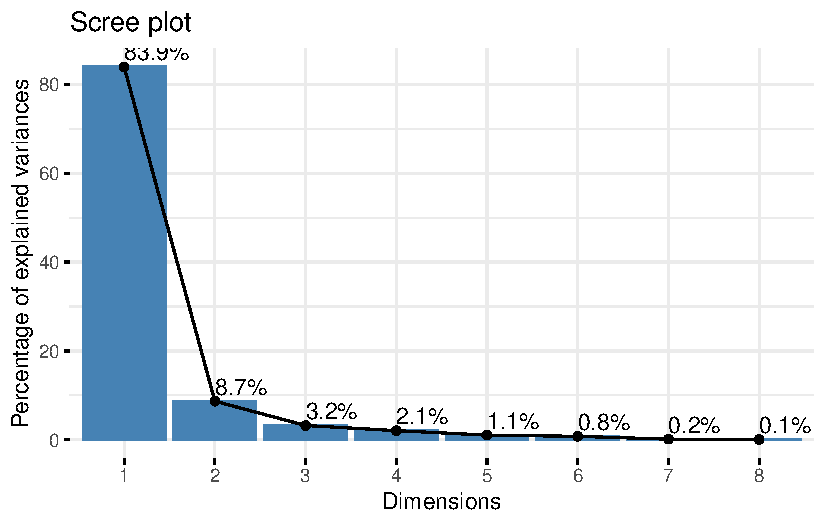
\includegraphics{examples_files/figure-pdf/unnamed-chunk-11-1.pdf}

}

\end{figure}

The scree plot visualizes the variance captured by each PC. PC1 explains
83.9\% of the variance, and PC2 explains 8.7\% variance.

\hypertarget{biplot}{%
\subsubsection{Biplot}\label{biplot}}

The correlation between a variable and a principal component is used as
the coordinates of the variable on the PC, shown as dimensions on the
biplot. Dim1 corresponds to PC1, and Dim2 to PC2. The representation of
variables differs from the plot of the observations: The observations
are represented by their projections, but the variables are represented
by their correlations {[}10{]}.

\begin{Shaded}
\begin{Highlighting}[]
\FunctionTok{fviz\_pca\_biplot}\NormalTok{(abalone\_pca, }\AttributeTok{label =} \StringTok{"var"}\NormalTok{, }\AttributeTok{alpha.ind =} \StringTok{"contrib"}\NormalTok{, }\AttributeTok{col.var =} \StringTok{"blue"}\NormalTok{, }\AttributeTok{repel =} \ConstantTok{TRUE}\NormalTok{)}
\end{Highlighting}
\end{Shaded}

\begin{figure}[H]

{\centering 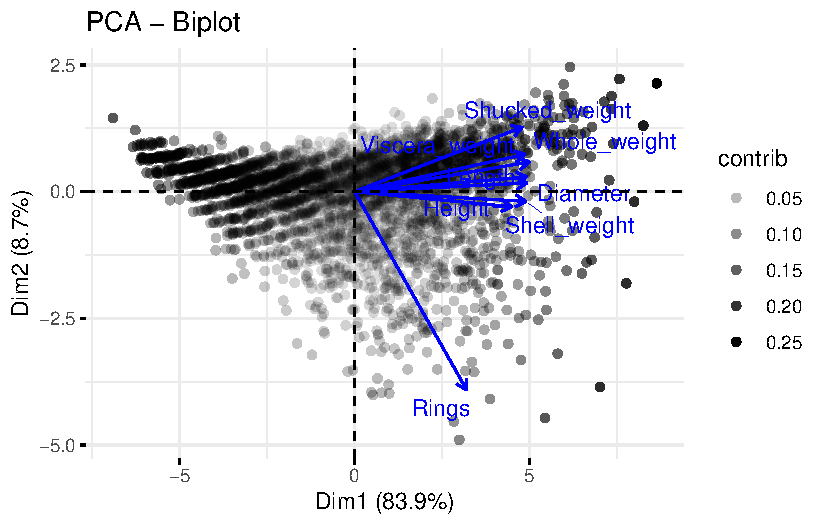
\includegraphics{examples_files/figure-pdf/unnamed-chunk-12-1.pdf}

}

\end{figure}

\hypertarget{variable-contribution}{%
\subsubsection{Variable Contribution}\label{variable-contribution}}

Top variable contribution for the first two principal components.

\begin{Shaded}
\begin{Highlighting}[]
\CommentTok{\# Contributions of variables to PC1}
\NormalTok{pc2\_contribution }\OtherTok{\textless{}{-}} \FunctionTok{fviz\_contrib}\NormalTok{(abalone\_pca, }\AttributeTok{choice =} \StringTok{"var"}\NormalTok{, }\AttributeTok{axes =} \DecValTok{1}\NormalTok{, }\AttributeTok{top =} \DecValTok{20}\NormalTok{)}

\CommentTok{\# Modify the theme to rotate X{-}axis labels to 90 degrees}
\NormalTok{pc2\_contribution }\SpecialCharTok{+}
  \FunctionTok{theme}\NormalTok{(}
    \AttributeTok{axis.text.x =} \FunctionTok{element\_text}\NormalTok{(}\AttributeTok{angle =} \DecValTok{0}\NormalTok{),}
    \AttributeTok{plot.title =} \FunctionTok{element\_text}\NormalTok{(}\AttributeTok{hjust =} \DecValTok{0}\NormalTok{)  }\CommentTok{\# horizontal justification}
\NormalTok{  ) }\SpecialCharTok{+}
  \FunctionTok{coord\_flip}\NormalTok{() }\SpecialCharTok{+}
  \FunctionTok{labs}\NormalTok{(}\AttributeTok{title =} \StringTok{"Contribution of Variables to PC1"}\NormalTok{,}
       \AttributeTok{y =} \StringTok{"Percentage Contribution"}\NormalTok{,}
       \AttributeTok{x =} \StringTok{""}\NormalTok{,}
       \AttributeTok{caption =} \StringTok{"PC1 explains 83.9\% of the variance"}\NormalTok{) }\SpecialCharTok{+}
  \FunctionTok{scale\_y\_continuous}\NormalTok{(}\AttributeTok{labels =}\NormalTok{ scales}\SpecialCharTok{::}\FunctionTok{percent\_format}\NormalTok{(}\AttributeTok{scale =} \DecValTok{1}\NormalTok{,}
                                                     \AttributeTok{accuracy =} \DecValTok{1}\NormalTok{))}
\end{Highlighting}
\end{Shaded}

\begin{figure}[H]

{\centering 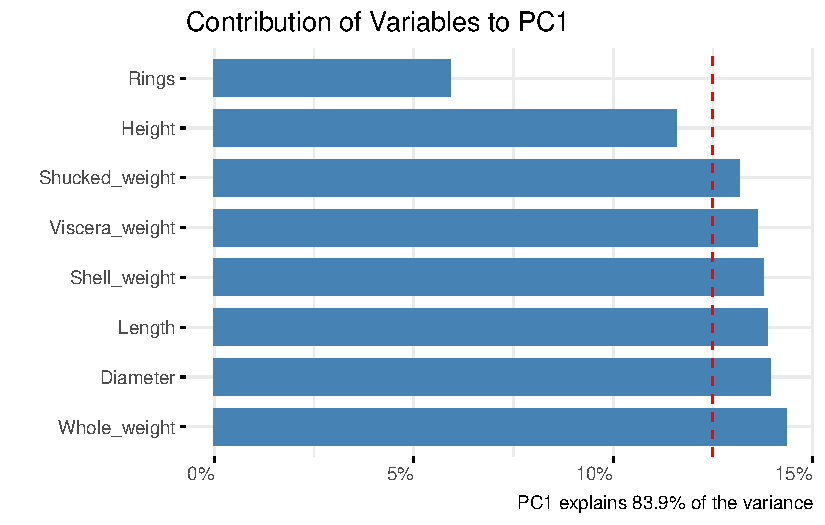
\includegraphics{examples_files/figure-pdf/unnamed-chunk-13-1.pdf}

}

\end{figure}

\begin{Shaded}
\begin{Highlighting}[]
\CommentTok{\# Contributions of variables to PC2}
\NormalTok{pc2\_contribution }\OtherTok{\textless{}{-}} \FunctionTok{fviz\_contrib}\NormalTok{(abalone\_pca, }\AttributeTok{choice =} \StringTok{"var"}\NormalTok{, }\AttributeTok{axes =} \DecValTok{2}\NormalTok{, }\AttributeTok{top =} \DecValTok{12}\NormalTok{)}

\CommentTok{\# Modify the theme to rotate X{-}axis labels to 90 degrees}
\NormalTok{pc2\_contribution }\SpecialCharTok{+}
  \FunctionTok{theme}\NormalTok{(}
    \AttributeTok{axis.text.x =} \FunctionTok{element\_text}\NormalTok{(}\AttributeTok{angle =} \DecValTok{0}\NormalTok{),}
    \AttributeTok{plot.title =} \FunctionTok{element\_text}\NormalTok{(}\AttributeTok{hjust =} \DecValTok{0}\NormalTok{)  }\CommentTok{\# horizontal justification}
\NormalTok{  ) }\SpecialCharTok{+}
  \FunctionTok{coord\_flip}\NormalTok{() }\SpecialCharTok{+}
  \FunctionTok{labs}\NormalTok{(}\AttributeTok{title =} \StringTok{"Contribution of Variables to PC2"}\NormalTok{,}
       \AttributeTok{y =} \StringTok{"Percentage Contribution"}\NormalTok{,}
       \AttributeTok{x =} \StringTok{""}\NormalTok{,}
       \AttributeTok{caption =} \StringTok{"PC2 explains 8.7\% of the variance"}\NormalTok{) }\SpecialCharTok{+}
  \FunctionTok{scale\_y\_continuous}\NormalTok{(}\AttributeTok{labels =}\NormalTok{ scales}\SpecialCharTok{::}\FunctionTok{percent\_format}\NormalTok{(}\AttributeTok{scale =} \DecValTok{1}\NormalTok{,}
                                                     \AttributeTok{accuracy =} \DecValTok{1}\NormalTok{))}
\end{Highlighting}
\end{Shaded}

\begin{figure}[H]

{\centering 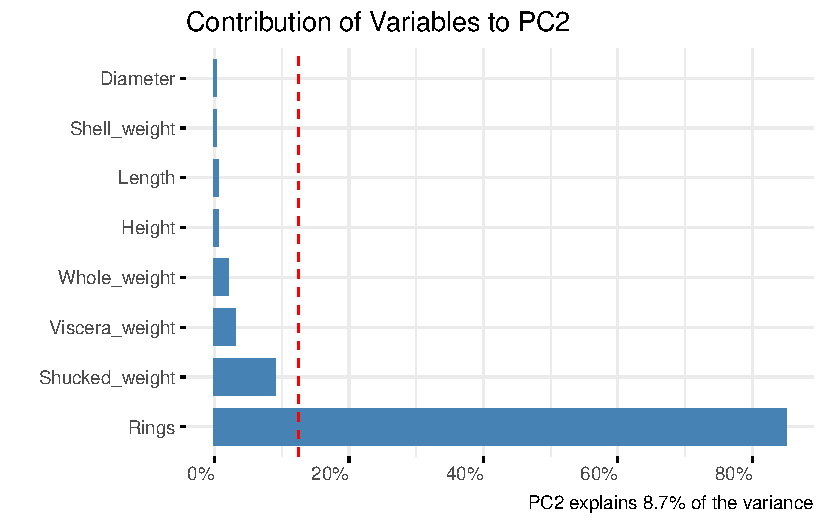
\includegraphics{examples_files/figure-pdf/unnamed-chunk-13-2.pdf}

}

\end{figure}

\hypertarget{results-1}{%
\subsection{Results}\label{results-1}}

The first principal component captures 83.9\% of the variance in the
data. This linear combination has relatively equal loadings for whole
weight, diameter, length, shell weight, viscera weight, and shucked
weight, with height and rings having lower loadings. The second
principal component is mostly influenced by the variable rings which
makes up over 80\% of the contribution to PC2. The biplot is an
effective visualization of how each variable contributes to PC1, or
dimension 1 on the graph, and PC2, or dimension 2 on the graph. The
length and direction of each vector represent the contribution of each
variable to the principal components; whole weight and rings are the
longest, representing the largest contributions to PC1 and PC2
respectively.

PCA is primarily an exploratory tool, which allows us to visualize
high-dimensional data in lower dimensions as shown above in the biplot
and accompanying scree plot. These PCs can be used to explore data in
other ways, such as looking for trends and patterns in the data or
identifying clusters and outliers. In the formal analysis in the
following chapter, the applications of PCA are further explored through
the development of a regression model on the principal components of a
dataset.

\bookmarksetup{startatroot}

\hypertarget{dataset}{%
\chapter{Dataset}\label{dataset}}

This is where we can put everything about our dataset description and
visualization.

The principal data used in this analysis was obtained from the
``Consumer Assessment of Healthcare Providers and Systems (CAHPS)
In-Center Hemodialysis Survey'', which is administered to in-center
hemodialysis (ICH) facilities by approved survey vendors under the
Centers for Medicare \& Medicaid Services (CMS). The dataset comprises
39 variables consisting of state-level averages of common dialysis
quality measures. The version in this analysis was released on July 19,
2023 through the data.cms.gov website. {[}24{]}

The structure of the dataset can be categorized into three main
components:

\begin{enumerate}
\def\labelenumi{\arabic{enumi}.}
\tightlist
\item
  Index Variable: The primary index variable is ``State,'' encompassing
  all 50 states and 6 U.S. territories, namely American Samoa, the
  District of Columbia, Guam, the Northern Mariana Islands, Puerto Rico,
  and the U.S. Virgin Islands.
\item
  Response Variables: The dataset incorporates 24 response variables
  aligned with ratings of patient care quality in dialysis facilities.
  These variables pertain to various aspects of dialysis procedures,
  such as transfusions, fistula usage, infections, hospitalizations,
  incident patient waitlisting, and readmissions.
\item
  Classification of Dialysis Patients: Fourteen variables within the
  dataset classify dialysis patients based on parameters including
  dialysis adequacy (Kt/V), type of dialysis (hemodialysis
  vs.~peritoneal dialysis), normalized protein catabolic rate (nPCR),
  hypercalcemia level (Serum Calcium, Mg/dL), serum phosphorus level
  (Mg/dL), and average hemoglobin (Hgb) level.
\end{enumerate}

The selection of this dataset for our analysis is driven by its inherent
characteristic of multicollinearity among variables, indicating that
certain variables are less significant in explaining the variability of
the response variables. Additionally, all variables in the dataset are
numeric, except for the index variable that is excluded from the
subsequent Principal Component Analysis (PCA). Our objective is to
utilize this dataset to illustrate the efficacy of PCA in dimension
reduction and the efficient visualization of data.

\hypertarget{renaming-variables}{%
\section{Renaming Variables}\label{renaming-variables}}

In our data preparation process, we have efficiently removed white
spaces, and edited variable names, enhancing the readability and
interpretability of the dataset. This meticulous effort adds to the
overall clarity, making it quicker, and more meaningful for further
examination. For instance, ``hypercalcemia\_calcium \textgreater{}
10.2Mg'', was used in replacement of
Percentage.Of.Adult..Patients.With.Hypercalcemia..Serum.Calcium.Greater.Than.10.2.Mg.dL.

\hypertarget{statistical-summary}{%
\section{Statistical Summary}\label{statistical-summary}}

The dataset contains 56 observations of 39 variables with 1 discrete
variable (States/Territories) and 38 continuous variables. 13
observations have at least 1 missing record, with 34 missing
observations in total. Most missing data in the dataset occurs in
variables relating to pediatric patient data.

\begin{table}
\centering
\begin{tabular}[t]{l|l|l|l|l|l|l|l|l|l|l|l|l|l|l|l|l|l|l|l|l|l|l|l|l|l|l|l|l|l|l|l|l|l|l|l|l|l|l}
\hline
  & better\_fistula & better\_hospital\_readmission & better\_hospitalization & better\_infection & better\_survival & better\_transfusion & expected\_fistula & expected\_hospital\_readmission & expected\_hospitalization & expected\_infection & expected\_survival & expected\_transfusion & Hgb\_10g & Hgb\_12g & hypercalcemia\_calcium > 10.2Mg & incident\_transplant\_waitlist\_better & incident\_transplant\_waitlist\_expected & incident\_transplant\_waitlist\_worse & Kt\_v\_1.2 & Kt\_v\_1.7 & long\_term\_catheter & pediatric\_Kt\_v\_1.8 & pediatric\_nPCR & pedriatic\_Kt\_v\_1.2 & phosphorus (3.5 - 4.5) Mg & phosphorus (4.6 - 5.5) Mg & phosphorus (5.6 - 7) Mg & phosphorus < 3.5Mg & phosphorus > 7Mg & prevalent\_transplant\_waitlist\_better & prevalent\_transplant\_waitlist\_expected & prevalent\_transplant\_waitlist\_worse & worse\_fistula & worse\_hospital\_readmission & worse\_hospitalization & worse\_infection & worse\_survival & worse\_transfusion\\
\hline
Mean & 4.928571 & 2.446429 & 1.250000 & 40.000000 & 3.482143 & 0.1785714 & 116.571429 & 119.589286 & 122.964286 & 74.000000 & 118.928571 & 99.232143 & 21.4727273 & 0.2363636 & 2.4000000 & 4.714286 & 61.017857 & 2.857143 & 96.4000000 & 91.7222222 & 17.0181818 & 74.5434783 & 91.0196078 & 91.2040816 & 23.1272727 & 29.0909091 & 23.7090909 & 7.6000000 & 16.4545455 & 7.839286 & 120.910714 & 2.892857 & 5.250000 & 3.500000 & 4.928571 & 1.142857 & 4.125000 & 7.285714\\
\hline
Std.Dev & 9.444300 & 3.201816 & 2.225881 & 54.678232 & 5.134522 & 0.4712514 & 137.766714 & 143.414945 & 144.863442 & 80.787038 & 141.581824 & 120.253367 & 7.8689605 & 0.4287638 & 4.3316236 & 9.692948 & 84.743354 & 5.528204 & 1.8718183 & 4.3628650 & 3.9181010 & 23.3063716 & 14.8478823 & 10.3822356 & 2.4118116 & 1.6696942 & 1.5948148 & 1.0988209 & 3.0600059 & 24.430069 & 144.045735 & 3.530020 & 8.237939 & 6.266796 & 10.759955 & 1.710168 & 6.084444 & 9.415102\\
\hline
Min & 0.000000 & 0.000000 & 0.000000 & 0.000000 & 0.000000 & 0.0000000 & 0.000000 & 2.000000 & 1.000000 & 0.000000 & 2.000000 & 1.000000 & 9.0000000 & 0.0000000 & 1.0000000 & 0.000000 & 0.000000 & 0.000000 & 87.0000000 & 69.0000000 & 10.0000000 & 0.0000000 & 15.0000000 & 47.0000000 & 11.0000000 & 24.0000000 & 20.0000000 & 5.0000000 & 8.0000000 & 0.000000 & 0.000000 & 0.000000 & 0.000000 & 0.000000 & 0.000000 & 0.000000 & 0.000000 & 0.000000\\
\hline
Q1 & 0.000000 & 0.000000 & 0.000000 & 5.500000 & 0.000000 & 0.0000000 & 24.500000 & 22.500000 & 26.000000 & 13.000000 & 23.000000 & 21.500000 & 18.0000000 & 0.0000000 & 1.0000000 & 0.000000 & 8.500000 & 0.000000 & 96.0000000 & 90.0000000 & 15.0000000 & 64.0000000 & 89.0000000 & 86.0000000 & 22.0000000 & 28.0000000 & 23.0000000 & 7.0000000 & 15.0000000 & 0.000000 & 26.000000 & 0.000000 & 0.000000 & 0.000000 & 0.000000 & 0.000000 & 0.000000 & 1.000000\\
\hline
Median & 2.000000 & 1.500000 & 1.000000 & 22.000000 & 1.000000 & 0.0000000 & 66.000000 & 68.500000 & 71.500000 & 47.500000 & 67.500000 & 53.000000 & 20.0000000 & 0.0000000 & 2.0000000 & 1.000000 & 32.000000 & 1.000000 & 97.0000000 & 93.0000000 & 17.0000000 & 80.5000000 & 96.0000000 & 93.0000000 & 23.0000000 & 29.0000000 & 24.0000000 & 8.0000000 & 16.0000000 & 1.000000 & 63.000000 & 2.000000 & 1.000000 & 1.000000 & 1.000000 & 0.000000 & 1.000000 & 3.000000\\
\hline
Q3 & 5.500000 & 3.500000 & 2.000000 & 52.000000 & 4.500000 & 0.0000000 & 158.500000 & 157.500000 & 169.500000 & 107.000000 & 161.000000 & 135.500000 & 23.0000000 & 0.0000000 & 2.0000000 & 4.500000 & 80.000000 & 3.000000 & 97.0000000 & 94.0000000 & 18.0000000 & 93.0000000 & 100.0000000 & 100.0000000 & 24.0000000 & 30.0000000 & 24.0000000 & 8.0000000 & 18.0000000 & 4.000000 & 168.000000 & 4.500000 & 7.000000 & 3.000000 & 4.500000 & 2.000000 & 5.000000 & 10.500000\\
\hline
Max & 50.000000 & 17.000000 & 15.000000 & 290.000000 & 24.000000 & 2.0000000 & 659.000000 & 665.000000 & 675.000000 & 397.000000 & 657.000000 & 596.000000 & 60.0000000 & 1.0000000 & 33.0000000 & 52.000000 & 420.000000 & 34.000000 & 99.0000000 & 96.0000000 & 29.0000000 & 100.0000000 & 100.0000000 & 100.0000000 & 27.0000000 & 32.0000000 & 29.0000000 & 11.0000000 & 26.0000000 & 168.000000 & 714.000000 & 18.000000 & 40.000000 & 38.000000 & 67.000000 & 8.000000 & 24.000000 & 47.000000\\
\hline
MAD & 2.965200 & 2.223900 & 1.482600 & 26.686800 & 1.482600 & 0.0000000 & 76.353900 & 80.801700 & 83.025600 & 54.856200 & 77.095200 & 62.269200 & 4.4478000 & 0.0000000 & 1.4826000 & 1.482600 & 42.995400 & 1.482600 & 1.4826000 & 2.9652000 & 2.9652000 & 20.0151000 & 5.9304000 & 10.3782000 & 1.4826000 & 1.4826000 & 1.4826000 & 1.4826000 & 2.9652000 & 1.482600 & 77.836500 & 2.965200 & 1.482600 & 1.482600 & 1.482600 & 0.000000 & 1.482600 & 4.447800\\
\hline
IQR & 5.250000 & 3.250000 & 2.000000 & 45.250000 & 4.250000 & 0.0000000 & 132.500000 & 133.000000 & 142.250000 & 92.500000 & 136.500000 & 111.500000 & 5.0000000 & 0.0000000 & 1.0000000 & 4.250000 & 70.250000 & 3.000000 & 1.0000000 & 4.0000000 & 3.0000000 & 28.5000000 & 10.5000000 & 14.0000000 & 2.0000000 & 2.0000000 & 1.0000000 & 1.0000000 & 3.0000000 & 4.000000 & 139.000000 & 4.250000 & 6.500000 & 3.000000 & 4.250000 & 2.000000 & 5.000000 & 9.250000\\
\hline
CV & 1.916235 & 1.308771 & 1.780705 & 1.366956 & 1.474529 & 2.6390081 & 1.181822 & 1.199229 & 1.178094 & 1.091717 & 1.190478 & 1.211839 & 0.3664630 & 1.8140006 & 1.8048432 & 2.056080 & 1.388829 & 1.934871 & 0.0194172 & 0.0475661 & 0.2302303 & 0.3126547 & 0.1631284 & 0.1138352 & 0.1042843 & 0.0573957 & 0.0672660 & 0.1445817 & 0.1859672 & 3.116364 & 1.191340 & 1.220254 & 1.569131 & 1.790513 & 2.183179 & 1.496397 & 1.475017 & 1.292269\\
\hline
Skewness & 3.363870 & 2.328926 & 4.353682 & 2.635591 & 2.262096 & 2.5829463 & 2.096187 & 2.093319 & 2.107653 & 1.777830 & 2.136469 & 2.309874 & 2.7370740 & 1.2073920 & 6.4192747 & 3.542913 & 2.726188 & 3.655246 & -2.8903292 & -2.8380628 & 1.0385708 & -1.2724094 & -3.1559206 & -1.8528969 & -2.2926951 & -0.6565867 & 0.8481480 & 0.3256139 & 0.1880386 & 5.267453 & 2.055601 & 1.901652 & 2.014739 & 3.383665 & 3.960928 & 1.795458 & 1.956831 & 2.220536\\
\hline
SE.Skewness & 0.319000 & 0.319000 & 0.319000 & 0.319000 & 0.319000 & 0.3190000 & 0.319000 & 0.319000 & 0.319000 & 0.319000 & 0.319000 & 0.319000 & 0.3217421 & 0.3217421 & 0.3217421 & 0.319000 & 0.319000 & 0.319000 & 0.3217421 & 0.3245563 & 0.3217421 & 0.3500963 & 0.3334641 & 0.3398276 & 0.3217421 & 0.3217421 & 0.3217421 & 0.3217421 & 0.3217421 & 0.319000 & 0.319000 & 0.319000 & 0.319000 & 0.319000 & 0.319000 & 0.319000 & 0.319000 & 0.319000\\
\hline
Kurtosis & 11.890419 & 6.698317 & 23.383843 & 7.991801 & 5.329195 & 5.9771465 & 4.759628 & 4.725274 & 4.912233 & 3.576431 & 4.953014 & 6.086035 & 10.0996967 & -0.5512415 & 42.3098624 & 12.933033 & 8.090744 & 16.044548 & 11.3474387 & 11.4686782 & 1.5698513 & 1.4283998 & 11.9801099 & 4.7877933 & 9.5790499 & 0.5666625 & 1.2609791 & 0.5920821 & 1.7100296 & 30.444720 & 4.657044 & 4.550810 & 4.184155 & 14.260341 & 18.224998 & 3.260659 & 3.107099 & 5.961102\\
\hline
N.Valid & 56.000000 & 56.000000 & 56.000000 & 56.000000 & 56.000000 & 56.0000000 & 56.000000 & 56.000000 & 56.000000 & 56.000000 & 56.000000 & 56.000000 & 55.0000000 & 55.0000000 & 55.0000000 & 56.000000 & 56.000000 & 56.000000 & 55.0000000 & 54.0000000 & 55.0000000 & 46.0000000 & 51.0000000 & 49.0000000 & 55.0000000 & 55.0000000 & 55.0000000 & 55.0000000 & 55.0000000 & 56.000000 & 56.000000 & 56.000000 & 56.000000 & 56.000000 & 56.000000 & 56.000000 & 56.000000 & 56.000000\\
\hline
Pct.Valid & 100.000000 & 100.000000 & 100.000000 & 100.000000 & 100.000000 & 100.0000000 & 100.000000 & 100.000000 & 100.000000 & 100.000000 & 100.000000 & 100.000000 & 98.2142857 & 98.2142857 & 98.2142857 & 100.000000 & 100.000000 & 100.000000 & 98.2142857 & 96.4285714 & 98.2142857 & 82.1428571 & 91.0714286 & 87.5000000 & 98.2142857 & 98.2142857 & 98.2142857 & 98.2142857 & 98.2142857 & 100.000000 & 100.000000 & 100.000000 & 100.000000 & 100.000000 & 100.000000 & 100.000000 & 100.000000 & 100.000000\\
\hline
\end{tabular}
\end{table}

The histograms of the data reveal that majority of the variables are
skewed right, with the QQ plots supporting that very few of the
variables are normally distributed. Finally, many of the variables are
highly correlated as expected based on the design of the dataset.

\hypertarget{missing-values-detection}{%
\section{Missing Values Detection}\label{missing-values-detection}}

\begin{itemize}
\tightlist
\item
  The 34 missing observations represent 1.6\% of the dataset.
\item
  14 variables have missing observations.
\item
  A table was generated to count missing values for all variables.
\end{itemize}

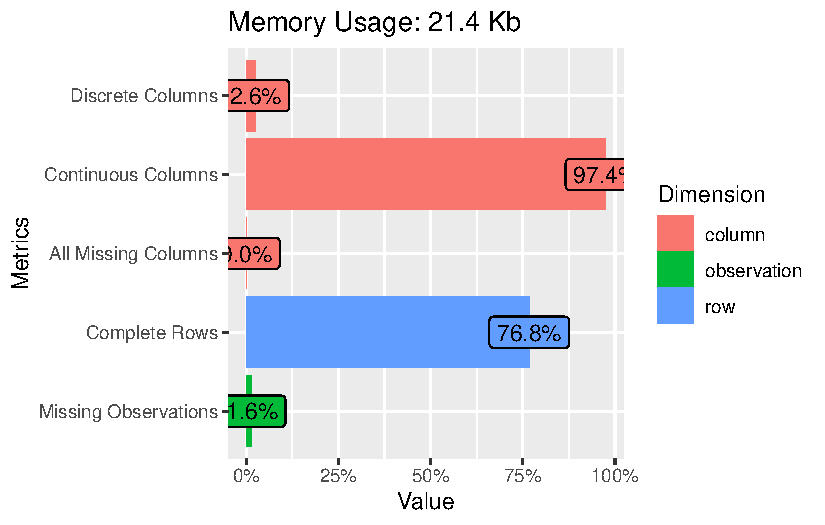
\includegraphics{dataset_files/figure-pdf/unnamed-chunk-5-1.pdf}

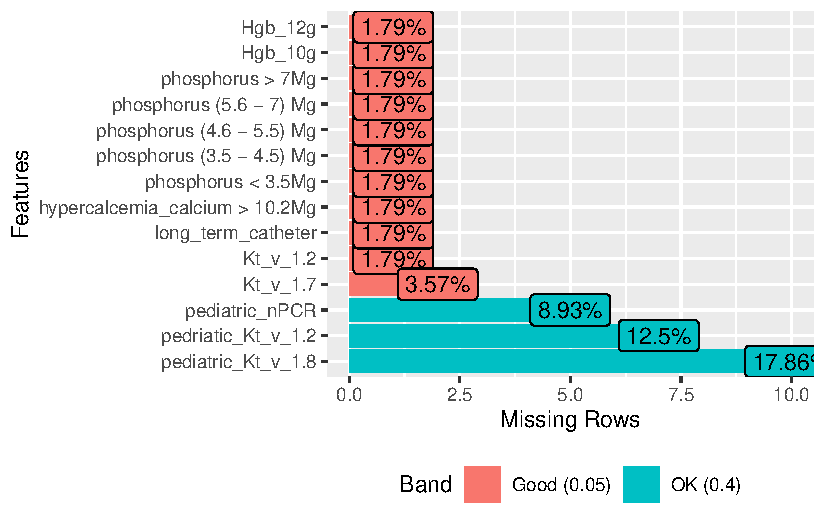
\includegraphics{dataset_files/figure-pdf/unnamed-chunk-5-2.pdf}

\begin{table}
\centering
\begin{tabular}[t]{l|r}
\hline
  & Missing\_Values\\
\hline
State & 0\\
\hline
better\_transfusion & 0\\
\hline
expected\_transfusion & 0\\
\hline
worse\_transfusion & 0\\
\hline
better\_infection & 0\\
\hline
expected\_infection & 0\\
\hline
worse\_infection & 0\\
\hline
Kt\_v\_1.2 & 1\\
\hline
Kt\_v\_1.7 & 2\\
\hline
pedriatic\_Kt\_v\_1.2 & 7\\
\hline
pediatric\_Kt\_v\_1.8 & 10\\
\hline
pediatric\_nPCR & 5\\
\hline
better\_fistula & 0\\
\hline
expected\_fistula & 0\\
\hline
worse\_fistula & 0\\
\hline
long\_term\_catheter & 1\\
\hline
hypercalcemia\_calcium > 10.2Mg & 1\\
\hline
phosphorus < 3.5Mg & 1\\
\hline
phosphorus (3.5 - 4.5) Mg & 1\\
\hline
phosphorus (4.6 - 5.5) Mg & 1\\
\hline
phosphorus (5.6 - 7) Mg & 1\\
\hline
phosphorus > 7Mg & 1\\
\hline
better\_hospitalization & 0\\
\hline
expected\_hospitalization & 0\\
\hline
worse\_hospitalization & 0\\
\hline
better\_hospital\_readmission & 0\\
\hline
expected\_hospital\_readmission & 0\\
\hline
worse\_hospital\_readmission & 0\\
\hline
better\_survival & 0\\
\hline
expected\_survival & 0\\
\hline
worse\_survival & 0\\
\hline
incident\_transplant\_waitlist\_better & 0\\
\hline
incident\_transplant\_waitlist\_expected & 0\\
\hline
incident\_transplant\_waitlist\_worse & 0\\
\hline
prevalent\_transplant\_waitlist\_better & 0\\
\hline
prevalent\_transplant\_waitlist\_expected & 0\\
\hline
prevalent\_transplant\_waitlist\_worse & 0\\
\hline
Hgb\_10g & 1\\
\hline
Hgb\_12g & 1\\
\hline
\end{tabular}
\end{table}

\hypertarget{data-distribution}{%
\section{Data Distribution}\label{data-distribution}}

\begin{itemize}
\item
  Histograms were used to display a sample (8 variables) of the
  distribution in respect to the predictor variable.
\item
  Normality is not assumed. The majority of the observations in each
  variable do not meet the normality assumption.

  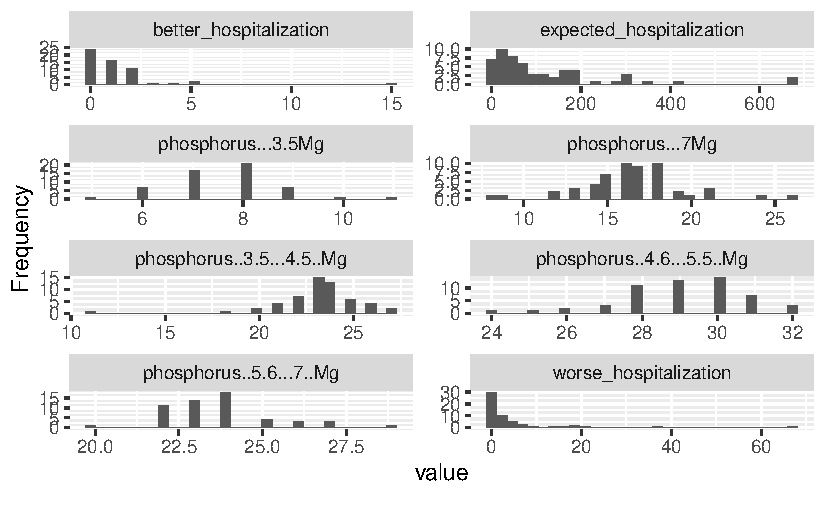
\includegraphics{dataset_files/figure-pdf/unnamed-chunk-7-1.pdf}
\end{itemize}

\hypertarget{normal-qq-plot-of-residuals}{%
\section{Normal QQ Plot of
Residuals}\label{normal-qq-plot-of-residuals}}

\begin{itemize}
\item
  It is apparent that the variables have heavy left and right tails.
\item
  The presence of outliers is consistent though the entire dataset.

  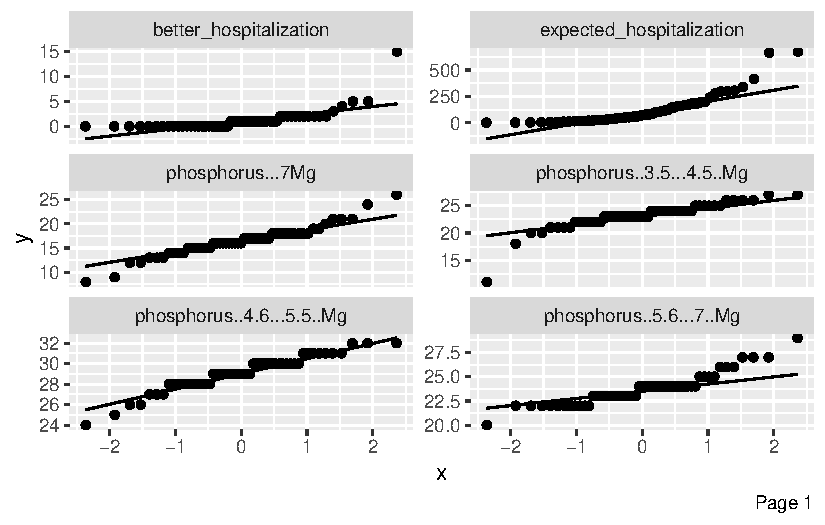
\includegraphics{dataset_files/figure-pdf/unnamed-chunk-8-1.pdf}

  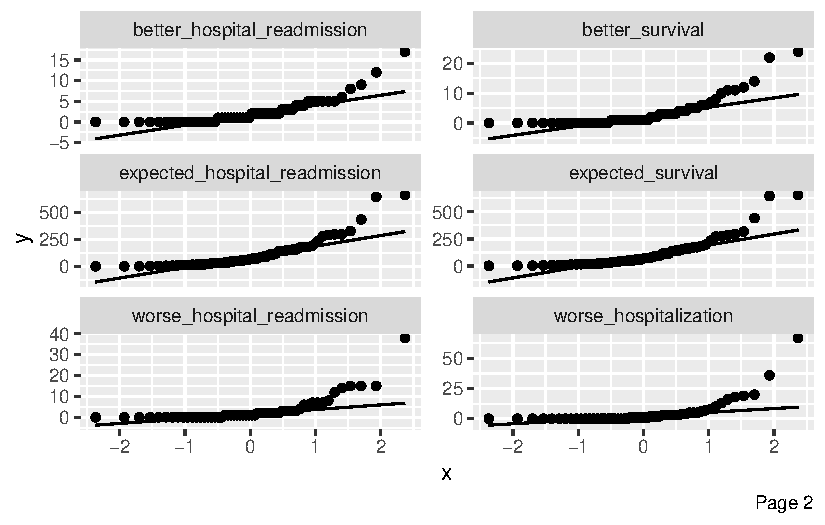
\includegraphics{dataset_files/figure-pdf/unnamed-chunk-8-2.pdf}
\end{itemize}

\hypertarget{imputation-of-missing-values}{%
\section{Imputation of Missing
Values}\label{imputation-of-missing-values}}

\begin{itemize}
\item
  After substituting missing values with the mean, we are now able to
  proceed with standardizing the dataset.
\item
  The standardization process will be implemented in the Analysis
  chapter.
\item
  A table was created to confirm the absence of any missing observations
  in the data frame.
\item
  Due to its categorical data type, the ``State'' variable was omitted
  from the analysis.
\end{itemize}

\begin{table}
\centering
\begin{tabular}[t]{l|r|l}
\hline
  & Missing\_Values & Type\\
\hline
better\_transfusion & 0 & double\\
\hline
expected\_transfusion & 0 & double\\
\hline
worse\_transfusion & 0 & double\\
\hline
better\_infection & 0 & double\\
\hline
expected\_infection & 0 & double\\
\hline
worse\_infection & 0 & double\\
\hline
Kt\_v\_1.2 & 0 & double\\
\hline
Kt\_v\_1.7 & 0 & double\\
\hline
pedriatic\_Kt\_v\_1.2 & 0 & double\\
\hline
pediatric\_Kt\_v\_1.8 & 0 & double\\
\hline
pediatric\_nPCR & 0 & double\\
\hline
better\_fistula & 0 & double\\
\hline
expected\_fistula & 0 & double\\
\hline
worse\_fistula & 0 & double\\
\hline
long\_term\_catheter & 0 & double\\
\hline
hypercalcemia\_calcium > 10.2Mg & 0 & double\\
\hline
phosphorus < 3.5Mg & 0 & double\\
\hline
phosphorus (3.5 - 4.5) Mg & 0 & double\\
\hline
phosphorus (4.6 - 5.5) Mg & 0 & double\\
\hline
phosphorus (5.6 - 7) Mg & 0 & double\\
\hline
phosphorus > 7Mg & 0 & double\\
\hline
better\_hospitalization & 0 & double\\
\hline
expected\_hospitalization & 0 & double\\
\hline
worse\_hospitalization & 0 & double\\
\hline
better\_hospital\_readmission & 0 & double\\
\hline
expected\_hospital\_readmission & 0 & double\\
\hline
worse\_hospital\_readmission & 0 & double\\
\hline
better\_survival & 0 & double\\
\hline
expected\_survival & 0 & double\\
\hline
worse\_survival & 0 & double\\
\hline
incident\_transplant\_waitlist\_better & 0 & double\\
\hline
incident\_transplant\_waitlist\_expected & 0 & double\\
\hline
incident\_transplant\_waitlist\_worse & 0 & double\\
\hline
prevalent\_transplant\_waitlist\_better & 0 & double\\
\hline
prevalent\_transplant\_waitlist\_expected & 0 & double\\
\hline
prevalent\_transplant\_waitlist\_worse & 0 & double\\
\hline
Hgb\_10g & 0 & double\\
\hline
Hgb\_12g & 0 & double\\
\hline
\end{tabular}
\end{table}

In conclusion, the dataset has undergone essential pre-processing steps,
rendering it well-prepared for outliers detection and normalization,
which are crucial for robust and accurate model development. Missing
observations have been imputed using the mean, ensuring that all
variables within the dataset are now numerical. These preliminary steps
have not only enhanced the dataset completeness, but also set the stage
for further advanced data analysis.

\bookmarksetup{startatroot}

\hypertarget{analysis}{%
\chapter{Analysis}\label{analysis}}

\hypertarget{data-preparation-1}{%
\section{Data Preparation}\label{data-preparation-1}}

This analysis uses the Dialysis dataset introduced previously in the
Dataset chapter. Within this context, we restructured the variables,
enhancing their meaningfulness and facilitating inferential analysis.
Additionally, the mean imputation approach addressed missing values.

\hypertarget{assumptions-1}{%
\section{Assumptions}\label{assumptions-1}}

PCA relies on certain assumptions, the fulfillment of which is essential
for the validity of this technique.

\begin{itemize}
\item
  \textbf{Linearity}: PCA assumes that the dataset is a linear
  combination of the variables. The variables exhibit relationships
  among themselves {[}25{]}.
\item
  \textbf{Importance of mean and covariance}: PCA assumes that the
  directions of maximum variance will contain good features for
  discrimination.
\item
  \textbf{Correlation between features}: PCA assumes a correlation
  between features.
\item
  \textbf{Normalization of data}: Normalization of data is necessary to
  apply PCA. Unscaled data can cause relative comparison problems of the
  dataset {[}25{]}. In addition, the data should contain no significant
  outliers.
\item
  \textbf{Orthogonality}: The principal components are orthogonal to
  each other.
\item
  \textbf{Sampling adequacy}: PCA assumes that there is sampling
  adequacy.
\end{itemize}

\hypertarget{feature-scaling-1}{%
\section{Feature Scaling}\label{feature-scaling-1}}

\hypertarget{standardization}{%
\subsection{Standardization}\label{standardization}}

It is important to Mean-Center the data prior to PCA model building to
ensure the first Principal Component is in the direction of maximum
variance.

\begin{itemize}
\item
  Standardization produces Mean, \(\mu\)= 0, and Standard Deviation,
  \(\sigma\) = 1.
\item
  We can rewrite this as:

  \[
  Z = \frac{{x - \mu}}{{\sigma}}
  \]

  \[
  Z \sim N(0,1)
  \]
\end{itemize}

\begin{Shaded}
\begin{Highlighting}[]
\CommentTok{\# Find the index position of the target feature }
\NormalTok{target\_name }\OtherTok{\textless{}{-}} \StringTok{"expected\_survival"}
\NormalTok{target\_index }\OtherTok{\textless{}{-}} \FunctionTok{grep}\NormalTok{(target\_name, }
                     \FunctionTok{colnames}\NormalTok{(train\_data))}
\end{Highlighting}
\end{Shaded}

\begin{Shaded}
\begin{Highlighting}[]
\CommentTok{\# Standardization Numerical Features}
\NormalTok{train\_data\_sc }\OtherTok{\textless{}{-}} \FunctionTok{scale}\NormalTok{(train\_data[, }\SpecialCharTok{{-}}\NormalTok{target\_index])}
\end{Highlighting}
\end{Shaded}

\hypertarget{pca-requirements}{%
\section{PCA Requirements}\label{pca-requirements}}

\hypertarget{outliers-detection}{%
\subsection{Outliers Detection}\label{outliers-detection}}

\begin{itemize}
\tightlist
\item
  There are some outliers in the data frame including the dependent
  variable.
\item
  However, there are three outliers with no high leverage.
\item
  Outliers are important because these can have a disproportionate
  influence on results.
\end{itemize}

\begin{Shaded}
\begin{Highlighting}[]
\CommentTok{\# Plot a boxplot to visualize potential outliers}
\FunctionTok{boxplot}\NormalTok{(train\_data, }\AttributeTok{main =} \StringTok{"Outliers Detection"}\NormalTok{,}
        \AttributeTok{col =} \StringTok{"steelblue"}\NormalTok{)}
\end{Highlighting}
\end{Shaded}

\begin{figure}[H]

{\centering 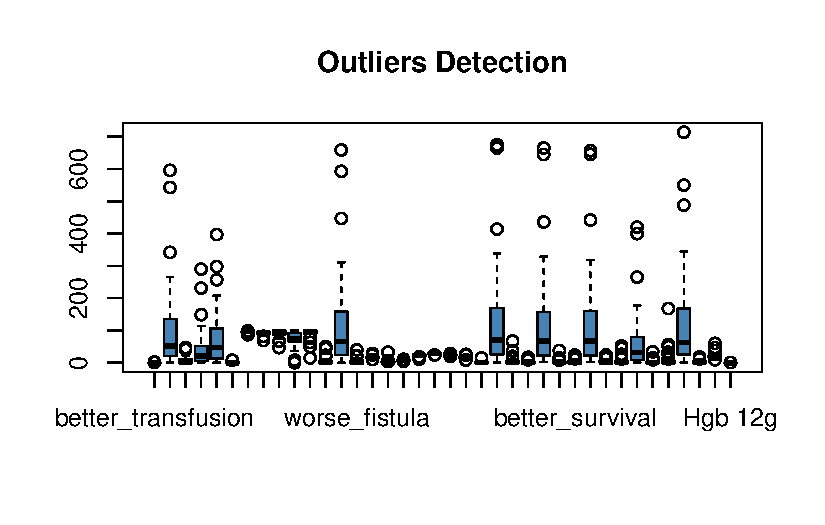
\includegraphics{analysis_files/figure-pdf/unnamed-chunk-9-1.pdf}

}

\end{figure}

\begin{Shaded}
\begin{Highlighting}[]
\CommentTok{\# Dependent Variable outliers}
\NormalTok{train\_data }\SpecialCharTok{\%\textgreater{}\%} 
  \FunctionTok{ggplot}\NormalTok{(}\FunctionTok{aes}\NormalTok{(}\AttributeTok{y=}\NormalTok{expected\_survival)) }\SpecialCharTok{+}
  \FunctionTok{geom\_boxplot}\NormalTok{(}\AttributeTok{fill=}\StringTok{"steelblue"}\NormalTok{, }\AttributeTok{alpha=}\FloatTok{0.75}\NormalTok{) }\SpecialCharTok{+} 
  \FunctionTok{xlab}\NormalTok{(}\StringTok{"Expected Survival"}\NormalTok{)}\SpecialCharTok{+}
  \FunctionTok{ylab}\NormalTok{(}\StringTok{""}\NormalTok{)}\SpecialCharTok{+}
  \FunctionTok{ggtitle}\NormalTok{(}\StringTok{"Dependent Variable Outliers"}\NormalTok{)}
\end{Highlighting}
\end{Shaded}

\begin{figure}[H]

{\centering 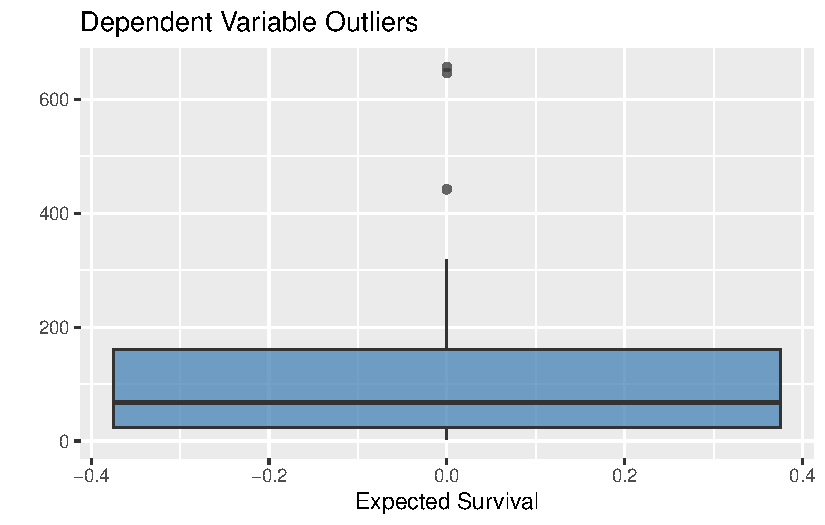
\includegraphics{analysis_files/figure-pdf/unnamed-chunk-10-1.pdf}

}

\end{figure}

\hypertarget{leverage}{%
\subsection{Leverage}\label{leverage}}

\begin{Shaded}
\begin{Highlighting}[]
\FunctionTok{set.seed}\NormalTok{(my\_seed)}

\CommentTok{\# Fit regression model}
\NormalTok{ordinary\_model }\OtherTok{\textless{}{-}} \FunctionTok{lm}\NormalTok{(expected\_survival }\SpecialCharTok{\textasciitilde{}}\NormalTok{ ., }\AttributeTok{data =}\NormalTok{ train\_data)}

\CommentTok{\# Print the model summary}
\FunctionTok{summary}\NormalTok{(ordinary\_model)}

\CommentTok{\# Residual Diagnostics}
\FunctionTok{ols\_plot\_resid\_lev}\NormalTok{(ordinary\_model)}
\end{Highlighting}
\end{Shaded}

\begin{figure}[H]

{\centering 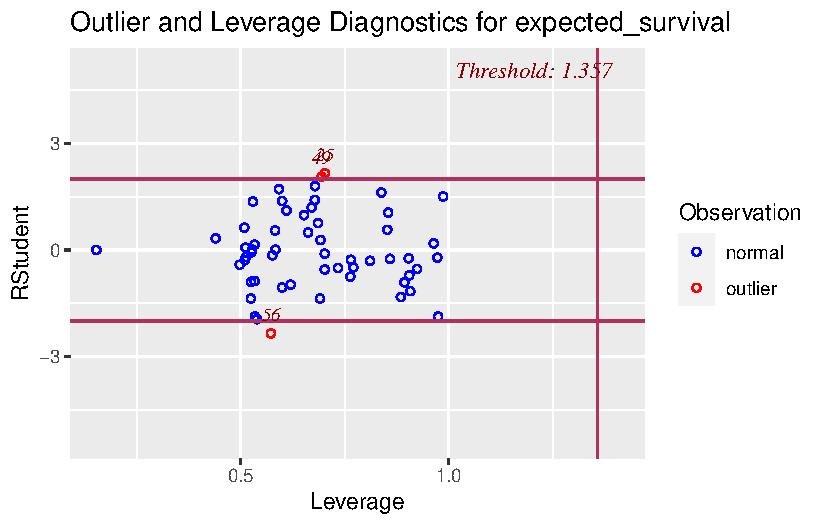
\includegraphics{analysis_files/figure-pdf/unnamed-chunk-11-1.pdf}

}

\end{figure}

\hypertarget{removing-outliers}{%
\subsection{Removing Outliers}\label{removing-outliers}}

After removing one outlier from the dataset, we discovered that the
final results produced minimal variability. Therefore, we decided to
present a model that captures all the data points' information; thus, no
observations will be removed from the final model.

\begin{Shaded}
\begin{Highlighting}[]
\CommentTok{\# No Outliers subset}
\NormalTok{no\_outliers\_df }\OtherTok{\textless{}{-}} \FunctionTok{slice}\NormalTok{(train\_data, }\SpecialCharTok{{-}}\FunctionTok{c}\NormalTok{(}\DecValTok{56}\NormalTok{))}

\FunctionTok{set.seed}\NormalTok{(my\_seed)}

\CommentTok{\# Fit regression model}
\NormalTok{no\_outliers\_model }\OtherTok{\textless{}{-}} \FunctionTok{lm}\NormalTok{(expected\_survival }\SpecialCharTok{\textasciitilde{}}\NormalTok{ ., }\AttributeTok{data =}\NormalTok{ no\_outliers\_df)}

\CommentTok{\# Print the model summary}
\FunctionTok{summary}\NormalTok{(no\_outliers\_model)}

\CommentTok{\# Residual Diagnostics}
\FunctionTok{ols\_plot\_resid\_lev}\NormalTok{(no\_outliers\_model)}
\end{Highlighting}
\end{Shaded}

\begin{figure}[H]

{\centering 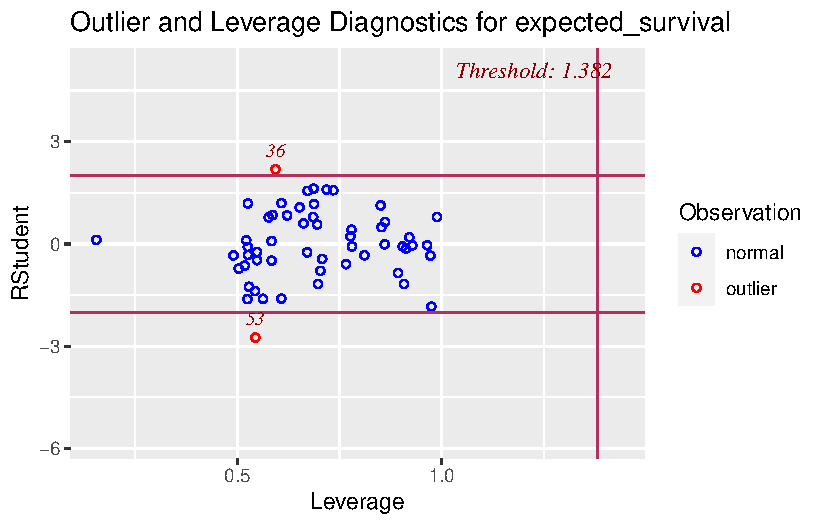
\includegraphics{analysis_files/figure-pdf/unnamed-chunk-12-1.pdf}

}

\end{figure}

\hypertarget{correlations}{%
\subsection{Correlations}\label{correlations}}

\begin{itemize}
\item
  Multicollinearity is present in the data set.
\item
  28 Correlated features were identified using a threshold = 0.30.
\end{itemize}

\begin{Shaded}
\begin{Highlighting}[]
\CommentTok{\# Calculate correlations and round to 2 digits}
\NormalTok{corr\_matrix }\OtherTok{\textless{}{-}} \FunctionTok{cor}\NormalTok{(train\_data\_sc)}
\NormalTok{corr\_matrix }\OtherTok{\textless{}{-}} \FunctionTok{round}\NormalTok{(corr\_matrix, }\AttributeTok{digits =} \DecValTok{2}\NormalTok{)}

\CommentTok{\# Print names of highly correlated features; threshold \textgreater{} 0.30}
\NormalTok{high }\OtherTok{\textless{}{-}} \FunctionTok{findCorrelation}\NormalTok{(corr\_matrix, }\AttributeTok{cutoff =} \FloatTok{0.30}\NormalTok{, }\AttributeTok{names =} \ConstantTok{TRUE}\NormalTok{)}

\CommentTok{\# Create a data frame with an index column}
\NormalTok{high\_corr\_df }\OtherTok{\textless{}{-}} \FunctionTok{data.frame}\NormalTok{(}
  \AttributeTok{Count =} \DecValTok{1}\SpecialCharTok{:}\FunctionTok{length}\NormalTok{(high),}
  \AttributeTok{Feature =}\NormalTok{ high}
\NormalTok{)}

\CommentTok{\# table format}
\FunctionTok{kbl}\NormalTok{(high\_corr\_df, }\AttributeTok{caption =} \StringTok{"Highly Correlated Features"}\NormalTok{) }\SpecialCharTok{\%\textgreater{}\%}
  \FunctionTok{kable\_paper}\NormalTok{(}\StringTok{"hover"}\NormalTok{)}
\end{Highlighting}
\end{Shaded}

\begin{table}

\caption{Highly Correlated Features}
\centering
\begin{tabular}[t]{r|l}
\hline
Count & Feature\\
\hline
1 & expected\_transfusion\\
\hline
2 & better\_infection\\
\hline
3 & expected\_hospitalization\\
\hline
4 & expected\_hospital\_readmission\\
\hline
5 & expected\_fistula\\
\hline
6 & prevalent\_transplant\_waitlist\_expected\\
\hline
7 & incident\_transplant\_waitlist\_expected\\
\hline
8 & expected\_infection\\
\hline
9 & worse\_survival\\
\hline
10 & incident\_transplant\_waitlist\_better\\
\hline
11 & better\_hospital\_readmission\\
\hline
12 & worse\_transfusion\\
\hline
13 & worse\_hospital\_readmission\\
\hline
14 & worse\_fistula\\
\hline
15 & incident\_transplant\_waitlist\_worse\\
\hline
16 & better\_fistula\\
\hline
17 & prevalent\_transplant\_waitlist\_better\\
\hline
18 & better\_survival\\
\hline
19 & worse\_infection\\
\hline
20 & phosphorus (5.6 - 7) Mg\\
\hline
21 & prevalent\_transplant\_waitlist\_worse\\
\hline
22 & phosphorus (3.5 - 4.5) Mg\\
\hline
23 & phosphorus > 7Mg\\
\hline
24 & better\_transfusion\\
\hline
25 & Hgb 10g\\
\hline
26 & hypercalcemia\_calcium > 10.2Mg\\
\hline
27 & pediatric\_nPCR\\
\hline
28 & long\_term\_catheter\\
\hline
\end{tabular}
\end{table}

\begin{Shaded}
\begin{Highlighting}[]
\NormalTok{corrplot}\SpecialCharTok{::}\FunctionTok{corrplot}\NormalTok{(corr\_matrix, }\AttributeTok{type =} \StringTok{"full"}\NormalTok{, }\AttributeTok{tl.pos =} \StringTok{"n"}\NormalTok{)}
\end{Highlighting}
\end{Shaded}

\begin{figure}[H]

{\centering 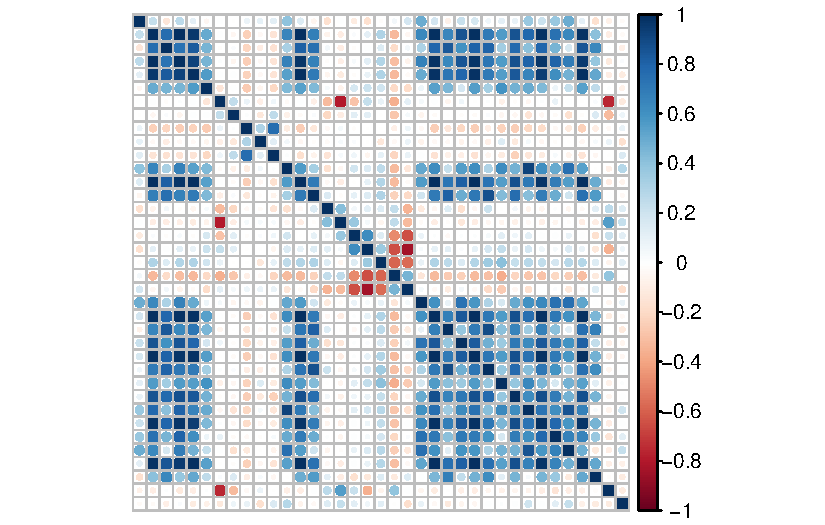
\includegraphics{analysis_files/figure-pdf/unnamed-chunk-14-1.pdf}

}

\end{figure}

\hypertarget{full-model-regression}{%
\section{Full Model Regression}\label{full-model-regression}}

\begin{itemize}
\tightlist
\item
  The Adjusted \(R^2\) = 99.99\% is an indication of over-fitting, or
  high variance.
\item
  This dataset is suitable to apply PCA to find the adequate variance
  balance.
\end{itemize}

\begin{Shaded}
\begin{Highlighting}[]
\FunctionTok{set.seed}\NormalTok{(my\_seed)}

\CommentTok{\# Fit a multiple linear regression model}
\NormalTok{full\_model }\OtherTok{\textless{}{-}} \FunctionTok{lm}\NormalTok{(expected\_survival }\SpecialCharTok{\textasciitilde{}}\NormalTok{ ., }\AttributeTok{data =}\NormalTok{ train\_data)}

\CommentTok{\# Print a summary of the regression model}
\FunctionTok{tab\_model}\NormalTok{(full\_model, }\AttributeTok{title =} \StringTok{"Full Model Regression"}\NormalTok{, }
          \AttributeTok{string.p=}\StringTok{"P{-}value"}\NormalTok{, }\AttributeTok{string.stat =} \StringTok{"T{-}score"}\NormalTok{,}
          \AttributeTok{string.se =} \StringTok{"Std. Error"}\NormalTok{,}
          \AttributeTok{string.resp =} \StringTok{"Response"}\NormalTok{,}
          \AttributeTok{string.ci =} \StringTok{"Conf Int."}\NormalTok{,}
          \AttributeTok{show.se=}\NormalTok{T, }\AttributeTok{show.stat =}\NormalTok{ T,}
           \AttributeTok{CSS =} \FunctionTok{list}\NormalTok{(}
             \AttributeTok{css.depvarhead =} \StringTok{\textquotesingle{}font{-}weight: bold; text{-}align: left;\textquotesingle{}}\NormalTok{,}
             \AttributeTok{css.summary =} \StringTok{\textquotesingle{}color: \#10759B; font{-}weight: bold;\textquotesingle{}}
\NormalTok{           ))}
\end{Highlighting}
\end{Shaded}

\begin{longtable}[]{@{}
  >{\centering\arraybackslash}p{(\columnwidth - 10\tabcolsep) * \real{0.1667}}
  >{\centering\arraybackslash}p{(\columnwidth - 10\tabcolsep) * \real{0.1667}}
  >{\centering\arraybackslash}p{(\columnwidth - 10\tabcolsep) * \real{0.1667}}
  >{\centering\arraybackslash}p{(\columnwidth - 10\tabcolsep) * \real{0.1667}}
  >{\centering\arraybackslash}p{(\columnwidth - 10\tabcolsep) * \real{0.1667}}
  >{\centering\arraybackslash}p{(\columnwidth - 10\tabcolsep) * \real{0.1667}}@{}}
\caption{Full Model Regression}\tabularnewline
\toprule\noalign{}
\endfirsthead
\endhead
\bottomrule\noalign{}
\endlastfoot
~ &
\multicolumn{5}{>{\centering\arraybackslash}p{(\columnwidth - 10\tabcolsep) * \real{0.8333} + 8\tabcolsep}@{}}{%
expected\_survival} \\
Predictors & Estimates & Std. Error & Conf Int. & T-score & P-value \\
(Intercept) & 93.71 & 41.88 & 5.73~--~181.69 & 2.24 & \textbf{0.038} \\
better transfusion & 1.04 & 0.75 & -0.53~--~2.62 & 1.39 & 0.181 \\
expected transfusion & 0.00 & 0.03 & -0.07~--~0.07 & 0.03 & 0.974 \\
worse transfusion & 0.13 & 0.08 & -0.03~--~0.29 & 1.76 & 0.096 \\
better infection & -0.27 & 0.09 & -0.46~--~-0.07 & -2.92 &
\textbf{0.009} \\
expected infection & -0.04 & 0.06 & -0.17~--~0.09 & -0.57 & 0.574 \\
worse infection & -0.11 & 0.27 & -0.68~--~0.46 & -0.41 & 0.687 \\
Kt v 1 2 & 0.25 & 0.25 & -0.28~--~0.78 & 0.99 & 0.335 \\
Kt v 1 7 & -0.00 & 0.05 & -0.11~--~0.11 & -0.00 & 0.996 \\
pedriatic Kt v 1 2 & -0.04 & 0.03 & -0.11~--~0.03 & -1.21 & 0.241 \\
pediatric Kt v 1 8 & -0.02 & 0.01 & -0.04~--~0.00 & -1.89 & 0.076 \\
pediatric nPCR & 0.04 & 0.03 & -0.01~--~0.10 & 1.75 & 0.097 \\
better fistula & -0.18 & 0.11 & -0.41~--~0.04 & -1.73 & 0.101 \\
expected fistula & 0.01 & 0.08 & -0.15~--~0.16 & 0.08 & 0.935 \\
worse fistula & -0.03 & 0.11 & -0.25~--~0.19 & -0.28 & 0.780 \\
long term catheter & 0.31 & 0.07 & 0.16~--~0.47 & 4.19 &
\textbf{0.001} \\
\begin{minipage}[t]{\linewidth}\raggedright
hypercalcemia calcium \textgreater{}\\
10 2Mg\strut
\end{minipage} & -0.19 & 0.09 & -0.37~--~-0.00 & -2.13 &
\textbf{0.048} \\
phosphorus \textless{} 3 5Mg & 0.35 & 0.48 & -0.66~--~1.36 & 0.73 &
0.476 \\
phosphorus (3 5 - 4 5) Mg & -1.73 & 0.46 & -2.71~--~-0.76 & -3.73 &
\textbf{0.002} \\
phosphorus (4 6 - 5 5) Mg & -1.36 & 0.46 & -2.33~--~-0.40 & -2.97 &
\textbf{0.008} \\
phosphorus (5 6 - 7) Mg & -0.80 & 0.44 & -1.72~--~0.12 & -1.82 &
0.085 \\
phosphorus \textgreater{} 7Mg & -1.44 & 0.46 & -2.41~--~-0.48 & -3.15 &
\textbf{0.005} \\
better hospitalization & 0.08 & 0.32 & -0.59~--~0.76 & 0.26 & 0.797 \\
expected hospitalization & 0.70 & 0.15 & 0.38~--~1.03 & 4.55 &
\textbf{\textless0.001} \\
worse hospitalization & 0.52 & 0.22 & 0.05~--~0.98 & 2.34 &
\textbf{0.031} \\
\begin{minipage}[t]{\linewidth}\raggedright
better hospital\\
readmission\strut
\end{minipage} & 0.38 & 0.24 & -0.13~--~0.88 & 1.55 & 0.139 \\
\begin{minipage}[t]{\linewidth}\raggedright
expected hospital\\
readmission\strut
\end{minipage} & 0.31 & 0.13 & 0.03~--~0.60 & 2.34 & \textbf{0.031} \\
\begin{minipage}[t]{\linewidth}\raggedright
worse hospital\\
readmission\strut
\end{minipage} & 0.09 & 0.24 & -0.41~--~0.59 & 0.39 & 0.704 \\
better survival & -0.57 & 0.15 & -0.88~--~-0.27 & -3.94 &
\textbf{0.001} \\
worse survival & -0.91 & 0.14 & -1.20~--~-0.62 & -6.64 &
\textbf{\textless0.001} \\
\begin{minipage}[t]{\linewidth}\raggedright
incident transplant\\
waitlist better\strut
\end{minipage} & 0.01 & 0.13 & -0.27~--~0.29 & 0.09 & 0.926 \\
\begin{minipage}[t]{\linewidth}\raggedright
incident transplant\\
waitlist expected\strut
\end{minipage} & 0.03 & 0.04 & -0.05~--~0.12 & 0.82 & 0.421 \\
\begin{minipage}[t]{\linewidth}\raggedright
incident transplant\\
waitlist worse\strut
\end{minipage} & 0.31 & 0.12 & 0.06~--~0.56 & 2.61 & \textbf{0.018} \\
\begin{minipage}[t]{\linewidth}\raggedright
prevalent transplant\\
waitlist better\strut
\end{minipage} & 0.15 & 0.11 & -0.08~--~0.38 & 1.36 & 0.191 \\
\begin{minipage}[t]{\linewidth}\raggedright
prevalent transplant\\
waitlist expected\strut
\end{minipage} & 0.04 & 0.10 & -0.17~--~0.25 & 0.41 & 0.690 \\
\begin{minipage}[t]{\linewidth}\raggedright
prevalent transplant\\
waitlist worse\strut
\end{minipage} & 0.01 & 0.19 & -0.39~--~0.40 & 0.03 & 0.975 \\
Hgb 10g & -0.10 & 0.05 & -0.20~--~-0.00 & -2.14 & \textbf{0.046} \\
Hgb 12g & -0.36 & 0.66 & -1.75~--~1.04 & -0.54 & 0.597 \\
Observations &
\multicolumn{5}{>{\raggedright\arraybackslash}p{(\columnwidth - 10\tabcolsep) * \real{0.8333} + 8\tabcolsep}@{}}{%
56} \\
R\textsuperscript{2} / R\textsuperscript{2} adjusted &
\multicolumn{5}{>{\raggedright\arraybackslash}p{(\columnwidth - 10\tabcolsep) * \real{0.8333} + 8\tabcolsep}@{}}{%
1.000 / 1.000} \\
\end{longtable}

\hypertarget{pca-implementation}{%
\section{PCA Implementation}\label{pca-implementation}}

\hypertarget{svd---singular-value-decomposition}{%
\subsection{SVD - Singular Value
Decomposition}\label{svd---singular-value-decomposition}}

We will focus on Singular Value Decomposition which is a classic
approach for PCA analysis.

Singular Value Decomposition is a factorization technique used in linear
algebra to decompose a matrix into three matrices.

\begin{enumerate}
\def\labelenumi{\arabic{enumi}.}
\item
  \(L\): A matrix whose columns are the left singular vectors of the
  original matrix.
\item
  \(D\): A diagonal matrix whose entries are the singular values of the
  original matrix.
\item
  \(R\): A matrix whose columns are the right singular vectors of the
  original matrix.
\end{enumerate}

The SVD is closely related to the eigenvalue decomposition (EVD), which
is another factorization technique used in linear algebra. While the EVD
can only be applied to square matrices, the SVD can be applied to any
matrix, including rectangular matrices. The SVD is also more numerically
stable than the EVD, making it a preferred method for many applications.

\begin{itemize}
\tightlist
\item
  Note: The Spectral Decomposition approach is used with the princomp()
  function.
\end{itemize}

\begin{Shaded}
\begin{Highlighting}[]
\CommentTok{\# Apply PCA using prcomp()}
\NormalTok{data\_pca }\OtherTok{\textless{}{-}} \FunctionTok{prcomp}\NormalTok{(train\_data\_sc, }\AttributeTok{center =} \ConstantTok{TRUE}\NormalTok{, }\AttributeTok{scale. =} \ConstantTok{TRUE}\NormalTok{)}
\NormalTok{pca\_summ }\OtherTok{\textless{}{-}} \FunctionTok{summary}\NormalTok{(data\_pca)}\SpecialCharTok{$}\NormalTok{importance}

\CommentTok{\# Transpose the matrix}
\NormalTok{transposed\_pca\_summ }\OtherTok{\textless{}{-}} \FunctionTok{t}\NormalTok{(pca\_summ)}

\CommentTok{\# table format}
\FunctionTok{kbl}\NormalTok{(transposed\_pca\_summ, }\AttributeTok{caption =} \StringTok{"Pricipal Components Analysis"}\NormalTok{,}
    \AttributeTok{digits =} \DecValTok{4}\NormalTok{) }\SpecialCharTok{\%\textgreater{}\%}
  \FunctionTok{kable\_paper}\NormalTok{(}\StringTok{"hover"}\NormalTok{)}
\end{Highlighting}
\end{Shaded}

\begin{table}

\caption{Pricipal Components Analysis}
\centering
\begin{tabular}[t]{l|r|r|r}
\hline
  & Standard deviation & Proportion of Variance & Cumulative Proportion\\
\hline
PC1 & 3.8854 & 0.4080 & 0.4080\\
\hline
PC2 & 1.8717 & 0.0947 & 0.5027\\
\hline
PC3 & 1.8377 & 0.0913 & 0.5940\\
\hline
PC4 & 1.7487 & 0.0826 & 0.6766\\
\hline
PC5 & 1.4227 & 0.0547 & 0.7313\\
\hline
PC6 & 1.2508 & 0.0423 & 0.7736\\
\hline
PC7 & 1.1280 & 0.0344 & 0.8080\\
\hline
PC8 & 1.0933 & 0.0323 & 0.8403\\
\hline
PC9 & 0.9449 & 0.0241 & 0.8644\\
\hline
PC10 & 0.9081 & 0.0223 & 0.8867\\
\hline
PC11 & 0.8185 & 0.0181 & 0.9048\\
\hline
PC12 & 0.7790 & 0.0164 & 0.9212\\
\hline
PC13 & 0.6815 & 0.0126 & 0.9338\\
\hline
PC14 & 0.6366 & 0.0110 & 0.9447\\
\hline
PC15 & 0.5710 & 0.0088 & 0.9535\\
\hline
PC16 & 0.5055 & 0.0069 & 0.9604\\
\hline
PC17 & 0.5018 & 0.0068 & 0.9673\\
\hline
PC18 & 0.4884 & 0.0064 & 0.9737\\
\hline
PC19 & 0.4625 & 0.0058 & 0.9795\\
\hline
PC20 & 0.4169 & 0.0047 & 0.9842\\
\hline
PC21 & 0.3534 & 0.0034 & 0.9876\\
\hline
PC22 & 0.3247 & 0.0029 & 0.9904\\
\hline
PC23 & 0.2884 & 0.0022 & 0.9926\\
\hline
PC24 & 0.2604 & 0.0018 & 0.9945\\
\hline
PC25 & 0.2259 & 0.0014 & 0.9959\\
\hline
PC26 & 0.2149 & 0.0013 & 0.9971\\
\hline
PC27 & 0.1982 & 0.0011 & 0.9982\\
\hline
PC28 & 0.1670 & 0.0008 & 0.9989\\
\hline
PC29 & 0.1268 & 0.0004 & 0.9994\\
\hline
PC30 & 0.1091 & 0.0003 & 0.9997\\
\hline
PC31 & 0.0838 & 0.0002 & 0.9999\\
\hline
PC32 & 0.0509 & 0.0001 & 0.9999\\
\hline
PC33 & 0.0317 & 0.0000 & 1.0000\\
\hline
PC34 & 0.0287 & 0.0000 & 1.0000\\
\hline
PC35 & 0.0143 & 0.0000 & 1.0000\\
\hline
PC36 & 0.0081 & 0.0000 & 1.0000\\
\hline
PC37 & 0.0049 & 0.0000 & 1.0000\\
\hline
\end{tabular}
\end{table}

\hypertarget{pca---elements-1}{%
\subsection{PCA - Elements}\label{pca---elements-1}}

\begin{itemize}
\item
  The values in `\textbf{\texttt{data\_pca\$x\textasciigrave{}}} are the
  coordinates of each observation in the new principal component space.
  These coordinates are the scores for each observation along each
  principal component.
\item
  The eigenvectors of the covariance, or correlation matrix of the data
  represent the directions of maximum variance, or information in the
  dataset.
\end{itemize}

\begin{Shaded}
\begin{Highlighting}[]
\CommentTok{\# Principal Component scores vector}
\NormalTok{pc\_scores }\OtherTok{\textless{}{-}}\NormalTok{ data\_pca}\SpecialCharTok{$}\NormalTok{x}

\CommentTok{\# Std Deviation of Components}
\NormalTok{component\_sdev }\OtherTok{\textless{}{-}}\NormalTok{ data\_pca}\SpecialCharTok{$}\NormalTok{sdev}

\CommentTok{\# Eigenvector, or Loadings}
\NormalTok{pc\_loadings }\OtherTok{\textless{}{-}}\NormalTok{ data\_pca}\SpecialCharTok{$}\NormalTok{rotation}

\CommentTok{\# Mean of variables}
\NormalTok{component\_mean }\OtherTok{\textless{}{-}}\NormalTok{ data\_pca}\SpecialCharTok{$}\NormalTok{center }

\CommentTok{\# Scaling factor of Variables}
\NormalTok{component\_scale }\OtherTok{\textless{}{-}}\NormalTok{ data\_pca}\SpecialCharTok{$}\NormalTok{scale}
\end{Highlighting}
\end{Shaded}

\hypertarget{loadings-of-first-two-components}{%
\subsection{Loadings of First Two
Components}\label{loadings-of-first-two-components}}

\begin{itemize}
\tightlist
\item
  The loading `data\_pca\$rotation` are the weights assigned to each
  original variable for that particular principal component.
\end{itemize}

\begin{Shaded}
\begin{Highlighting}[]
\CommentTok{\# Access the loadings for the first two principal components}
\NormalTok{loadings\_first\_two\_components }\OtherTok{\textless{}{-}}\NormalTok{ pc\_loadings[, }\DecValTok{1}\SpecialCharTok{:}\DecValTok{2}\NormalTok{]}

\CommentTok{\# Print the loadings for the first two principal components}
\CommentTok{\# print(loadings\_first\_two\_components)}

\CommentTok{\# table format}
\FunctionTok{kbl}\NormalTok{(loadings\_first\_two\_components, }
    \AttributeTok{caption =} \StringTok{"Loadings of First Two Principal Components"}\NormalTok{,}
    \AttributeTok{digits =} \DecValTok{4}\NormalTok{) }\SpecialCharTok{\%\textgreater{}\%}
  \FunctionTok{kable\_paper}\NormalTok{(}\StringTok{"hover"}\NormalTok{)}
\end{Highlighting}
\end{Shaded}

\begin{table}

\caption{Loadings of First Two Principal Components}
\centering
\begin{tabular}[t]{l|r|r}
\hline
  & PC1 & PC2\\
\hline
better\_transfusion & 0.0506 & 0.0151\\
\hline
expected\_transfusion & 0.2536 & -0.0214\\
\hline
worse\_transfusion & 0.2058 & -0.1647\\
\hline
better\_infection & 0.2526 & -0.0073\\
\hline
expected\_infection & 0.2455 & -0.0652\\
\hline
worse\_infection & 0.1381 & 0.0637\\
\hline
Kt\_v\_1.2 & 0.0031 & 0.0081\\
\hline
Kt\_v\_1.7 & -0.0078 & 0.0444\\
\hline
pedriatic\_Kt\_v\_1.2 & -0.0636 & 0.0527\\
\hline
pediatric\_Kt\_v\_1.8 & -0.0139 & 0.0028\\
\hline
pediatric\_nPCR & -0.0394 & 0.0768\\
\hline
better\_fistula & 0.1701 & 0.1849\\
\hline
expected\_fistula & 0.2521 & -0.0558\\
\hline
worse\_fistula & 0.1932 & -0.0481\\
\hline
long\_term\_catheter & -0.0054 & 0.0409\\
\hline
hypercalcemia\_calcium > 10.2Mg & -0.0276 & 0.1049\\
\hline
phosphorus < 3.5Mg & 0.0161 & 0.3759\\
\hline
phosphorus (3.5 - 4.5) Mg & 0.0420 & 0.4258\\
\hline
phosphorus (4.6 - 5.5) Mg & 0.0888 & 0.2665\\
\hline
phosphorus (5.6 - 7) Mg & -0.0954 & -0.3297\\
\hline
phosphorus > 7Mg & -0.0293 & -0.4400\\
\hline
better\_hospitalization & 0.1555 & 0.0398\\
\hline
expected\_hospitalization & 0.2535 & -0.0353\\
\hline
worse\_hospitalization & 0.1863 & -0.1048\\
\hline
better\_hospital\_readmission & 0.2100 & -0.0462\\
\hline
expected\_hospital\_readmission & 0.2537 & -0.0414\\
\hline
worse\_hospital\_readmission & 0.2010 & -0.0432\\
\hline
better\_survival & 0.1523 & 0.1688\\
\hline
worse\_survival & 0.2288 & -0.0662\\
\hline
incident\_transplant\_waitlist\_better & 0.2016 & 0.1513\\
\hline
incident\_transplant\_waitlist\_expected & 0.2499 & -0.0578\\
\hline
incident\_transplant\_waitlist\_worse & 0.1913 & -0.0199\\
\hline
prevalent\_transplant\_waitlist\_better & 0.1618 & 0.1763\\
\hline
prevalent\_transplant\_waitlist\_expected & 0.2501 & -0.0703\\
\hline
prevalent\_transplant\_waitlist\_worse & 0.1202 & -0.2285\\
\hline
Hgb 10g & -0.0299 & -0.0804\\
\hline
Hgb 12g & -0.0006 & 0.1765\\
\hline
\end{tabular}
\end{table}

\hypertarget{pca---cumulative-variance}{%
\subsection{PCA - Cumulative Variance}\label{pca---cumulative-variance}}

\begin{Shaded}
\begin{Highlighting}[]
\CommentTok{\# Proportion of variance explained by each PC}
\NormalTok{variance\_explained }\OtherTok{\textless{}{-}}\NormalTok{ component\_sdev}\SpecialCharTok{\^{}}\DecValTok{2} \SpecialCharTok{/} \FunctionTok{sum}\NormalTok{(component\_sdev}\SpecialCharTok{\^{}}\DecValTok{2}\NormalTok{)}

\CommentTok{\# Cumulative proportion of variance explained}
\NormalTok{cumulative\_variance\_explained }\OtherTok{\textless{}{-}} \FunctionTok{cumsum}\NormalTok{(variance\_explained)}

\CommentTok{\# Create a data frame with an index column}
\NormalTok{cumulative\_variance\_explained\_df }\OtherTok{\textless{}{-}} \FunctionTok{data.frame}\NormalTok{(}
  \AttributeTok{Pincipal\_Component =} \DecValTok{1}\SpecialCharTok{:}\FunctionTok{length}\NormalTok{(cumulative\_variance\_explained),}
  \AttributeTok{Cumulative\_Variance\_Explained =}\NormalTok{ cumulative\_variance\_explained}
\NormalTok{)}

\CommentTok{\# Create a kable table with an index column}
\FunctionTok{kbl}\NormalTok{(cumulative\_variance\_explained\_df, }\AttributeTok{align =} \StringTok{"cl"}\NormalTok{,}
    \AttributeTok{caption =} \StringTok{"PCA: Cumulative Variance Explained"}\NormalTok{,}
    \AttributeTok{digits =} \DecValTok{4}\NormalTok{) }\SpecialCharTok{\%\textgreater{}\%}
  \FunctionTok{kable\_paper}\NormalTok{(}\StringTok{"hover"}\NormalTok{)}
\end{Highlighting}
\end{Shaded}

\begin{table}

\caption{PCA: Cumulative Variance Explained}
\centering
\begin{tabular}[t]{c|l}
\hline
Pincipal\_Component & Cumulative\_Variance\_Explained\\
\hline
1 & 0.4080\\
\hline
2 & 0.5027\\
\hline
3 & 0.5940\\
\hline
4 & 0.6766\\
\hline
5 & 0.7313\\
\hline
6 & 0.7736\\
\hline
7 & 0.8080\\
\hline
8 & 0.8403\\
\hline
9 & 0.8644\\
\hline
10 & 0.8867\\
\hline
11 & 0.9048\\
\hline
12 & 0.9212\\
\hline
13 & 0.9338\\
\hline
14 & 0.9447\\
\hline
15 & 0.9535\\
\hline
16 & 0.9604\\
\hline
17 & 0.9673\\
\hline
18 & 0.9737\\
\hline
19 & 0.9795\\
\hline
20 & 0.9842\\
\hline
21 & 0.9876\\
\hline
22 & 0.9904\\
\hline
23 & 0.9927\\
\hline
24 & 0.9945\\
\hline
25 & 0.9959\\
\hline
26 & 0.9971\\
\hline
27 & 0.9982\\
\hline
28 & 0.9989\\
\hline
29 & 0.9994\\
\hline
30 & 0.9997\\
\hline
31 & 0.9999\\
\hline
32 & 0.9999\\
\hline
33 & 1.0000\\
\hline
34 & 1.0000\\
\hline
35 & 1.0000\\
\hline
36 & 1.0000\\
\hline
37 & 1.0000\\
\hline
\end{tabular}
\end{table}

\hypertarget{pca---number-of-principal-components}{%
\subsection{PCA - Number of Principal
Components}\label{pca---number-of-principal-components}}

\begin{itemize}
\tightlist
\item
  We can conclude that 9 Principal Components explain 86\% of the
  variance.
\end{itemize}

\begin{Shaded}
\begin{Highlighting}[]
\CommentTok{\# Retain components that explain a percentage of the variance}
\NormalTok{num\_components }\OtherTok{\textless{}{-}} \FunctionTok{which}\NormalTok{(cumulative\_variance\_explained }\SpecialCharTok{\textgreater{}=} \FloatTok{0.86}\NormalTok{)[}\DecValTok{1}\NormalTok{]}

\CommentTok{\# Select the desired number of principal components}
\NormalTok{selected\_pcs }\OtherTok{\textless{}{-}}\NormalTok{ pc\_scores[, }\DecValTok{1}\SpecialCharTok{:}\NormalTok{num\_components]}

\CommentTok{\# table format}
\FunctionTok{kbl}\NormalTok{(selected\_pcs, }\AttributeTok{caption =} \StringTok{"Components Explaining 86\% Variance"}\NormalTok{,}
    \AttributeTok{digits =} \DecValTok{4}\NormalTok{) }\SpecialCharTok{\%\textgreater{}\%}
  \FunctionTok{kable\_paper}\NormalTok{(}\StringTok{"hover"}\NormalTok{, }\AttributeTok{full\_width =}\NormalTok{ F)}
\end{Highlighting}
\end{Shaded}

\textbackslash begin\{table\}

\textbackslash caption\{\label{tab:unnamed-chunk-20}Components
Explaining 86\% Variance\} \centering

\begin{tabular}[t]{r|r|r|r|r|r|r|r|r}
\hline
PC1 & PC2 & PC3 & PC4 & PC5 & PC6 & PC7 & PC8 & PC9\\
\hline
-3.1378 & 0.7718 & -0.7364 & -0.9222 & -0.3593 & 0.3854 & 1.7645 & 0.7137 & -1.2776\\
\hline
0.9109 & -1.3736 & -0.8907 & -0.0460 & 0.0228 & 0.3267 & 1.9095 & 0.3203 & 0.3158\\
\hline
-1.3650 & -1.7656 & -0.1449 & 0.2592 & -1.2857 & -0.3762 & -0.7856 & -0.9204 & -1.2626\\
\hline
-3.0594 & 0.3348 & -0.0141 & -0.1395 & 0.0920 & -0.2825 & -0.1286 & 0.1373 & 0.0780\\
\hline
-0.1991 & -0.2073 & -0.7149 & -1.3756 & -1.1993 & 0.0319 & 0.7499 & 0.7160 & -0.1954\\
\hline
15.2032 & 2.6187 & -7.7363 & 4.0519 & -0.8244 & -2.8218 & -0.3937 & 0.7540 & 0.1236\\
\hline
-1.1596 & 1.1216 & -0.7112 & -0.6842 & 0.2286 & -0.3821 & -0.5148 & -1.3731 & 0.5560\\
\hline
-1.7567 & 2.4464 & 0.2336 & -0.7871 & -0.1098 & -1.0603 & -0.1434 & -1.6411 & 1.1462\\
\hline
-2.5605 & 1.0785 & -0.0207 & -0.0018 & -0.2474 & 1.1930 & -0.1234 & 1.6484 & 1.1223\\
\hline
-2.2725 & 0.7670 & -0.0552 & -1.0045 & 2.4430 & -1.8092 & 1.3011 & 0.0402 & 0.7853\\
\hline
10.2101 & -3.0951 & 5.5631 & -2.7079 & -3.2328 & -1.4788 & -1.0195 & 0.3946 & 0.0182\\
\hline
5.1286 & -1.7705 & 1.7849 & -0.1628 & 0.5176 & -0.3672 & 1.2737 & 0.3839 & -0.1914\\
\hline
-3.4958 & -4.4206 & -3.1425 & 0.0404 & -0.7928 & 0.4217 & 0.1087 & -1.1395 & -1.5791\\
\hline
-1.7134 & 0.8230 & -1.9663 & -1.0871 & 0.7505 & 0.4357 & 1.1010 & 0.8853 & -1.1906\\
\hline
-1.9511 & 0.9075 & -0.3459 & -1.4707 & -0.7735 & -0.7810 & -1.0116 & -1.4774 & 0.2215\\
\hline
-2.6296 & 0.9149 & -0.5263 & -1.3484 & -0.9348 & 0.5181 & 0.3570 & 0.8863 & -0.4488\\
\hline
4.7463 & 0.3146 & 2.3709 & -0.2528 & 0.8329 & 1.4290 & -0.8492 & 0.0128 & -0.0479\\
\hline
0.3868 & -0.9290 & 0.6870 & -0.6117 & 1.5374 & -0.1113 & 0.2265 & 0.7691 & -0.8385\\
\hline
-1.6767 & 0.2850 & -0.9842 & -1.8133 & -0.8136 & 0.7518 & 0.8450 & -0.2605 & 0.7893\\
\hline
-0.7345 & -1.3222 & 0.3700 & -0.8448 & 2.0553 & -1.6018 & 0.7571 & -1.1866 & 1.6751\\
\hline
0.9393 & -0.6999 & -0.1399 & -0.5978 & -0.0203 & -0.0046 & 1.3170 & 0.4944 & 0.4746\\
\hline
-0.8326 & 1.5874 & -0.7312 & 0.2910 & 0.1199 & 1.1100 & -1.6455 & 1.1312 & -0.0448\\
\hline
0.8725 & 1.0451 & 0.2775 & 0.2175 & -0.6226 & 0.5429 & -0.2118 & 0.9699 & 1.6165\\
\hline
-2.7730 & 0.5328 & -0.3857 & -0.9341 & 0.8943 & -2.7237 & -0.4738 & -2.6266 & 1.1451\\
\hline
2.0146 & 0.0014 & 0.6403 & -0.6929 & -0.1677 & 0.4555 & -0.3840 & 0.2754 & 1.0045\\
\hline
-1.1376 & 0.6676 & 0.0612 & 0.2444 & -0.4465 & 0.9265 & -0.6966 & 0.9414 & 0.1757\\
\hline
0.1256 & -0.9951 & 1.1503 & -0.4897 & 0.7108 & 1.3854 & 0.0279 & -0.3615 & -0.4521\\
\hline
-3.6486 & -5.1247 & 0.0491 & 6.3322 & -1.4438 & 1.4726 & -0.7719 & -0.9060 & 2.9209\\
\hline
-0.3307 & 0.2793 & -0.0985 & -0.3388 & -0.5950 & -0.5761 & 2.0137 & 0.0524 & 0.9485\\
\hline
-3.1386 & -2.4847 & -2.0044 & 1.0661 & -0.5877 & -0.0292 & -0.7689 & -0.0432 & -0.9302\\
\hline
1.8304 & -0.8659 & -0.6292 & -0.2888 & -0.3585 & 1.1522 & 1.4099 & -0.2387 & 0.1117\\
\hline
-2.6300 & 1.8820 & 1.4790 & 1.5197 & 0.1484 & 0.9943 & 1.0138 & 1.7547 & -0.2904\\
\hline
-1.9654 & 1.4437 & 0.4239 & -1.4217 & 0.3452 & 0.1489 & 0.2267 & 0.8292 & 0.0537\\
\hline
-2.9434 & -0.4453 & -0.1869 & 0.0501 & -0.3471 & -0.3884 & -1.8441 & 0.4520 & 0.3853\\
\hline
1.9335 & 4.2274 & -1.5429 & -0.8354 & -0.5412 & 2.3739 & -0.2919 & 0.2478 & 0.0526\\
\hline
-1.4611 & 0.5551 & -1.4467 & -0.2732 & 0.4168 & -0.3335 & 0.0306 & 1.0760 & -0.1292\\
\hline
-1.6820 & -0.9253 & -0.3177 & -0.2737 & -0.7852 & 0.2036 & -0.4687 & 0.5302 & -0.4388\\
\hline
6.7595 & 3.6388 & 1.0562 & 2.3514 & 2.4970 & 3.4372 & -1.4276 & -3.6075 & -1.6018\\
\hline
3.4507 & -1.1824 & 2.5699 & -1.1129 & -0.0546 & 1.4361 & -0.6591 & -1.0345 & -0.1605\\
\hline
-1.0984 & -1.5241 & -0.5320 & -0.4777 & -0.9995 & -0.8030 & -0.1950 & -1.6084 & -0.6964\\
\hline
-1.9193 & -0.0165 & -1.0806 & -0.5872 & -0.6324 & -0.2014 & -1.3158 & -1.3027 & 0.1718\\
\hline
3.4962 & 1.5199 & 1.3109 & -0.3007 & 2.5985 & 1.0499 & -0.2313 & -0.0969 & 0.8464\\
\hline
-0.2522 & 3.0718 & 2.1407 & -1.9255 & -2.2719 & -3.4093 & -2.1544 & 0.2271 & -1.2587\\
\hline
-3.0135 & -0.6858 & -1.1712 & -0.8551 & -0.4428 & 0.8391 & -1.0039 & 0.4085 & -0.1121\\
\hline
0.3392 & -0.5133 & 0.0391 & -0.1766 & -0.5924 & 1.0593 & 1.1663 & 0.5207 & -0.3248\\
\hline
-2.1136 & 2.6100 & 0.5330 & -0.8478 & 0.0752 & 0.1416 & 1.0927 & -0.3588 & 1.3478\\
\hline
1.3707 & -2.9104 & 1.0848 & 1.3163 & 6.1381 & -2.1436 & 0.9717 & 0.1946 & -1.2873\\
\hline
13.0708 & -2.7257 & 0.4257 & -0.4752 & -0.7834 & 0.5789 & 0.9620 & 0.5196 & -0.2282\\
\hline
-2.6465 & -0.3807 & -0.6944 & 1.0365 & -0.9202 & 0.4536 & 0.2146 & -0.6048 & -0.7532\\
\hline
1.7505 & -0.1798 & -0.2689 & -0.3411 & 0.6075 & -0.7767 & -0.0058 & 0.2781 & 1.5233\\
\hline
-3.3725 & 3.5365 & 5.3271 & 7.7627 & -2.3163 & -1.7961 & 2.1724 & -0.1875 & -1.1131\\
\hline
-3.1242 & -1.0424 & 0.8044 & 2.1331 & 2.8559 & -0.9073 & -3.9502 & 3.0657 & -0.2529\\
\hline
-1.0177 & -1.6718 & -1.8286 & 0.3950 & -0.4653 & 0.8616 & -0.2457 & -0.1711 & -0.3817\\
\hline
-0.3396 & 0.7505 & 0.9596 & -0.3014 & 0.5726 & 0.0189 & -0.0433 & 0.0637 & 0.6271\\
\hline
-2.2360 & -0.6559 & 0.7765 & 0.2318 & -0.2785 & -0.3448 & -0.0371 & 0.7968 & -1.0752\\
\hline
-3.1511 & 0.1807 & -1.0702 & -0.4912 & -0.2143 & -0.6257 & 0.7831 & -1.3442 & -1.6736\\
\hline
\end{tabular}

\textbackslash end\{table\}

\hypertarget{visualization-1}{%
\section{Visualization}\label{visualization-1}}

\hypertarget{scree-plot---cumulative-variance-explained-1}{%
\subsection{Scree Plot - Cumulative Variance
Explained}\label{scree-plot---cumulative-variance-explained-1}}

\begin{itemize}
\item
  PC1 explains 40.8\% variance.
\item
  PC2 explains 9.5\% variance.
\end{itemize}

\begin{Shaded}
\begin{Highlighting}[]
\FunctionTok{fviz\_eig}\NormalTok{(data\_pca, }\AttributeTok{addlabels =} \ConstantTok{TRUE}\NormalTok{)}
\end{Highlighting}
\end{Shaded}

\begin{figure}[H]

{\centering 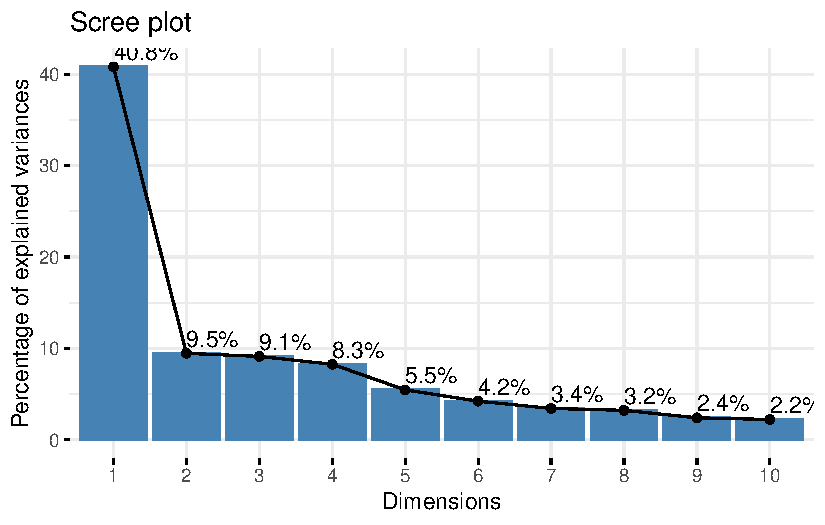
\includegraphics{analysis_files/figure-pdf/unnamed-chunk-21-1.pdf}

}

\end{figure}

\hypertarget{biplot-1}{%
\subsection{Biplot}\label{biplot-1}}

\begin{itemize}
\item
  The correlation between a variable and a principal component (PC) is
  used as the coordinates of the variable on the PC. The representation
  of variables differs from the plot of the observations: The
  observations are represented by their projections, but the variables
  are represented by their correlations {[}10{]}.
\item
  PC1 is represented in black which displays the longest distance of its
  projection.
\item
  PC2 is represented in blue which displays a shorter distance as
  expected.
\end{itemize}

\begin{Shaded}
\begin{Highlighting}[]
\FunctionTok{fviz\_pca\_biplot}\NormalTok{(data\_pca, }
                \AttributeTok{geom =} \FunctionTok{c}\NormalTok{(}\StringTok{"point"}\NormalTok{, }\StringTok{"arrow"}\NormalTok{),}
                \AttributeTok{geom.var =} \StringTok{"arrow"}\NormalTok{)}
\end{Highlighting}
\end{Shaded}

\begin{figure}[H]

{\centering 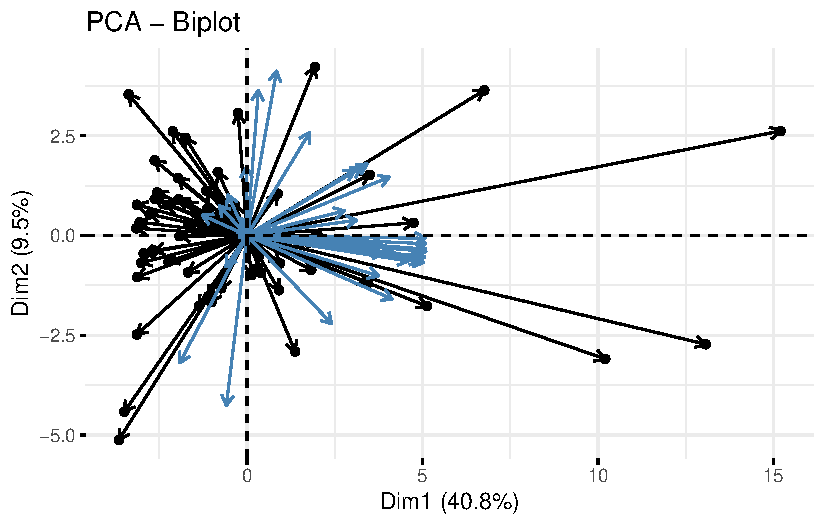
\includegraphics{analysis_files/figure-pdf/unnamed-chunk-22-1.pdf}

}

\end{figure}

\hypertarget{correlation-circle}{%
\subsection{Correlation Circle}\label{correlation-circle}}

The plot below is also known as variable correlation plots. It shows the
relationships between all variables. It can be interpreted as follow:

\begin{itemize}
\item
  Positively correlated variables are grouped together.
\item
  Negatively correlated variables are positioned on opposite sides of
  the plot origin (opposed quadrants).
\item
  The distance between variables and the origin measures the quality of
  the variables on the factor map. Variables that are away from the
  origin are well represented on the factor map.
\end{itemize}

\begin{Shaded}
\begin{Highlighting}[]
\CommentTok{\# Control variable colors using their contributions}
\FunctionTok{fviz\_pca\_var}\NormalTok{(data\_pca, }\AttributeTok{col.var =} \StringTok{"contrib"}\NormalTok{,}
   \AttributeTok{gradient.cols =} \FunctionTok{c}\NormalTok{(}\StringTok{"white"}\NormalTok{, }\StringTok{"blue"}\NormalTok{, }\StringTok{"red"}\NormalTok{),}
   \AttributeTok{geom.var =} \StringTok{"arrow"}\NormalTok{,}
   \AttributeTok{ggtheme =} \FunctionTok{theme\_minimal}\NormalTok{())}
\end{Highlighting}
\end{Shaded}

\begin{figure}[H]

{\centering 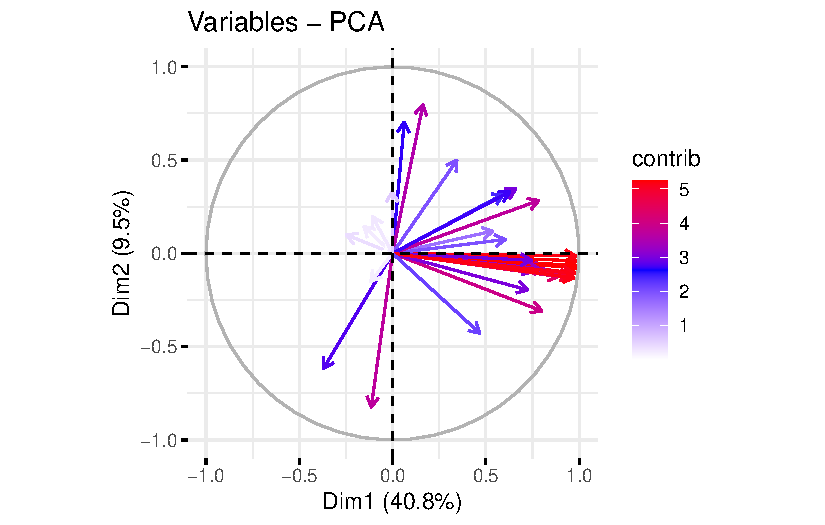
\includegraphics{analysis_files/figure-pdf/unnamed-chunk-23-1.pdf}

}

\end{figure}

\hypertarget{variable-contribution-1}{%
\subsection{Variable Contribution}\label{variable-contribution-1}}

Top variable contribution for the first two principal components.

\begin{Shaded}
\begin{Highlighting}[]
\CommentTok{\# Contributions of variables to PC1}
\NormalTok{pc2\_contribution }\OtherTok{\textless{}{-}} \FunctionTok{fviz\_contrib}\NormalTok{(data\_pca, }\AttributeTok{choice =} \StringTok{"var"}\NormalTok{, }\AttributeTok{axes =} \DecValTok{1}\NormalTok{, }\AttributeTok{top =} \DecValTok{20}\NormalTok{)}

\CommentTok{\# Modify the theme to rotate X{-}axis labels to 90 degrees}
\NormalTok{pc2\_contribution }\SpecialCharTok{+}
  \FunctionTok{theme}\NormalTok{(}
    \AttributeTok{axis.text.x =} \FunctionTok{element\_text}\NormalTok{(}\AttributeTok{angle =} \DecValTok{0}\NormalTok{),}
    \AttributeTok{plot.title =} \FunctionTok{element\_text}\NormalTok{(}\AttributeTok{hjust =} \DecValTok{0}\NormalTok{)  }\CommentTok{\# horizontal justification}
\NormalTok{  ) }\SpecialCharTok{+}
  \FunctionTok{coord\_flip}\NormalTok{() }\SpecialCharTok{+}
  \FunctionTok{labs}\NormalTok{(}\AttributeTok{title =} \StringTok{"Contribution of Variables to PC1"}\NormalTok{,}
       \AttributeTok{y =} \StringTok{"Percentage Contribution"}\NormalTok{,}
       \AttributeTok{x =} \StringTok{""}\NormalTok{,}
       \AttributeTok{caption =} \StringTok{"PC1 explains 40.8\% variance"}\NormalTok{) }\SpecialCharTok{+}
  \FunctionTok{scale\_y\_continuous}\NormalTok{(}\AttributeTok{labels =}\NormalTok{ scales}\SpecialCharTok{::}\FunctionTok{percent\_format}\NormalTok{(}\AttributeTok{scale =} \DecValTok{1}\NormalTok{,}
                                                     \AttributeTok{accuracy =} \DecValTok{1}\NormalTok{))}
\end{Highlighting}
\end{Shaded}

\begin{figure}[H]

{\centering 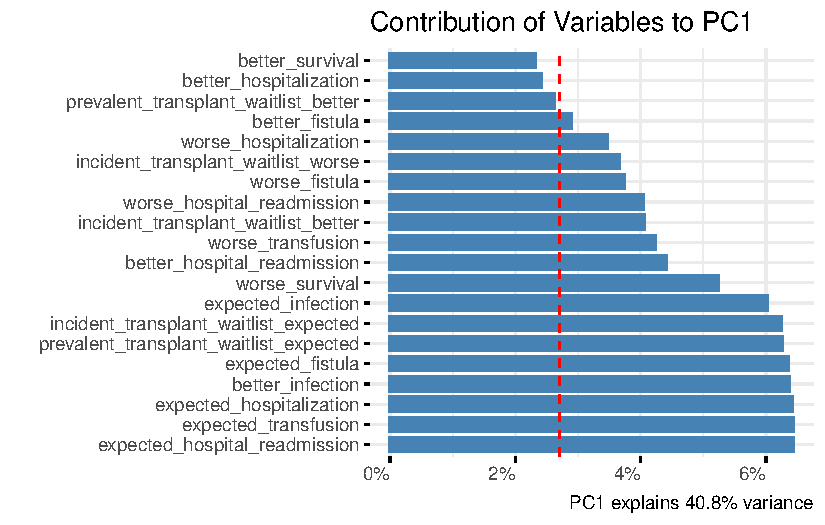
\includegraphics{analysis_files/figure-pdf/unnamed-chunk-24-1.pdf}

}

\end{figure}

\begin{Shaded}
\begin{Highlighting}[]
\CommentTok{\# Contributions of variables to PC2}
\NormalTok{pc2\_contribution }\OtherTok{\textless{}{-}} \FunctionTok{fviz\_contrib}\NormalTok{(data\_pca, }\AttributeTok{choice =} \StringTok{"var"}\NormalTok{, }\AttributeTok{axes =} \DecValTok{2}\NormalTok{, }\AttributeTok{top =} \DecValTok{12}\NormalTok{)}

\CommentTok{\# Modify the theme to rotate X{-}axis labels to 90 degrees}
\NormalTok{pc2\_contribution }\SpecialCharTok{+}
  \FunctionTok{theme}\NormalTok{(}
    \AttributeTok{axis.text.x =} \FunctionTok{element\_text}\NormalTok{(}\AttributeTok{angle =} \DecValTok{0}\NormalTok{),}
    \AttributeTok{plot.title =} \FunctionTok{element\_text}\NormalTok{(}\AttributeTok{hjust =} \DecValTok{0}\NormalTok{)  }\CommentTok{\# horizontal justification}
\NormalTok{  ) }\SpecialCharTok{+}
  \FunctionTok{coord\_flip}\NormalTok{() }\SpecialCharTok{+}
  \FunctionTok{labs}\NormalTok{(}\AttributeTok{title =} \StringTok{"Contribution of Variables to PC2"}\NormalTok{,}
       \AttributeTok{y =} \StringTok{"Percentage Contribution"}\NormalTok{,}
       \AttributeTok{x =} \StringTok{""}\NormalTok{,}
       \AttributeTok{caption =} \StringTok{"PC2 explains 9.5\% variance"}\NormalTok{) }\SpecialCharTok{+}
  \FunctionTok{scale\_y\_continuous}\NormalTok{(}\AttributeTok{labels =}\NormalTok{ scales}\SpecialCharTok{::}\FunctionTok{percent\_format}\NormalTok{(}\AttributeTok{scale =} \DecValTok{1}\NormalTok{,}
                                                     \AttributeTok{accuracy =} \DecValTok{1}\NormalTok{))}
\end{Highlighting}
\end{Shaded}

\begin{figure}[H]

{\centering 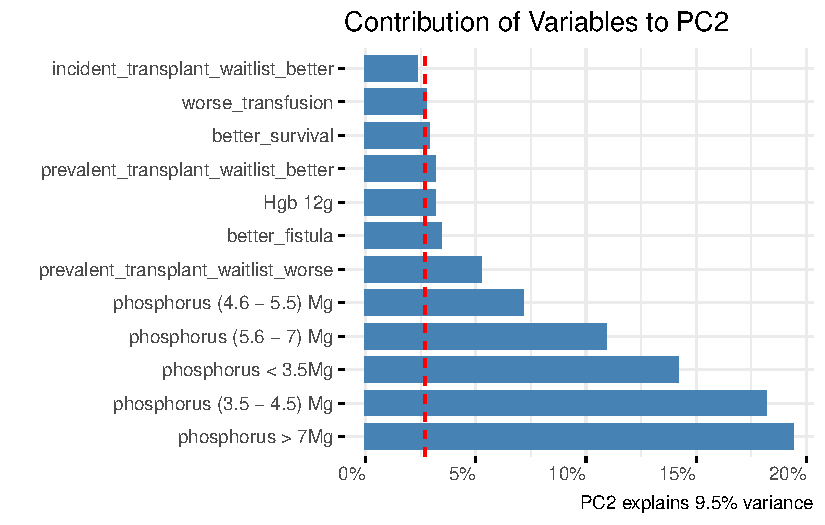
\includegraphics{analysis_files/figure-pdf/unnamed-chunk-24-2.pdf}

}

\end{figure}

\hypertarget{model-building}{%
\section{Model Building}\label{model-building}}

\hypertarget{data-splitting-into-training-test-set}{%
\subsection{Data Splitting into Training \& Test
set}\label{data-splitting-into-training-test-set}}

\begin{Shaded}
\begin{Highlighting}[]
\CommentTok{\# reproducible random sampling}
\FunctionTok{set.seed}\NormalTok{(my\_seed)  }
 
\CommentTok{\# Create Target y{-}variable for the training set}
\NormalTok{y }\OtherTok{\textless{}{-}}\NormalTok{ train\_data}\SpecialCharTok{$}\NormalTok{expected\_survival  }
\CommentTok{\# Split the data into training and test sets }
\NormalTok{split }\OtherTok{\textless{}{-}} \FunctionTok{sample.split}\NormalTok{(y, }\AttributeTok{SplitRatio =} \FloatTok{0.7}\NormalTok{) }
\NormalTok{training\_set }\OtherTok{\textless{}{-}} \FunctionTok{subset}\NormalTok{(train\_data, split }\SpecialCharTok{==} \ConstantTok{TRUE}\NormalTok{) }
\NormalTok{test\_set }\OtherTok{\textless{}{-}} \FunctionTok{subset}\NormalTok{(train\_data, split }\SpecialCharTok{==} \ConstantTok{FALSE}\NormalTok{) }
\end{Highlighting}
\end{Shaded}

\hypertarget{feature-scaling-standardization}{%
\subsection{Feature Scaling:
Standardization}\label{feature-scaling-standardization}}

\begin{itemize}
\tightlist
\item
  Standardization ensures all features are on the same scale, and this
  method is less sensitive to outliers.
\end{itemize}

\begin{Shaded}
\begin{Highlighting}[]
\CommentTok{\# Feature Scaling: Standardization}
\CommentTok{\# Perform centering and scaling on the training and test sets}
\NormalTok{sc }\OtherTok{\textless{}{-}} \FunctionTok{preProcess}\NormalTok{(training\_set[, }\SpecialCharTok{{-}}\NormalTok{target\_index], }
                 \AttributeTok{method =} \FunctionTok{c}\NormalTok{(}\StringTok{"center"}\NormalTok{, }\StringTok{"scale"}\NormalTok{))}
\NormalTok{training\_set[, }\SpecialCharTok{{-}}\NormalTok{target\_index] }\OtherTok{\textless{}{-}} \FunctionTok{predict}\NormalTok{(}
\NormalTok{  sc, training\_set[, }\SpecialCharTok{{-}}\NormalTok{target\_index])}
\NormalTok{test\_set[, }\SpecialCharTok{{-}}\NormalTok{target\_index] }\OtherTok{\textless{}{-}} \FunctionTok{predict}\NormalTok{(sc, test\_set[, }\SpecialCharTok{{-}}\NormalTok{target\_index])}
\end{Highlighting}
\end{Shaded}

\hypertarget{applying-pca-to-training-test-sets}{%
\subsection{Applying PCA to Training \& Test
sets}\label{applying-pca-to-training-test-sets}}

\begin{Shaded}
\begin{Highlighting}[]
\CommentTok{\# Perform Principal Component Analysis (PCA) preprocessing on the training data}
\NormalTok{pca }\OtherTok{\textless{}{-}} \FunctionTok{preProcess}\NormalTok{(training\_set[, }\SpecialCharTok{{-}}\NormalTok{target\_index], }
                  \AttributeTok{method =} \StringTok{\textquotesingle{}pca\textquotesingle{}}\NormalTok{, }\AttributeTok{pcaComp =} \DecValTok{8}\NormalTok{)}

\CommentTok{\# Apply PCA transformation to original training set}
\NormalTok{training\_set }\OtherTok{\textless{}{-}} \FunctionTok{predict}\NormalTok{(pca, training\_set)}

\CommentTok{\# Reorder columns, moving the dependent feature index to the end}
\NormalTok{training\_set }\OtherTok{\textless{}{-}}\NormalTok{ training\_set[}\FunctionTok{c}\NormalTok{(}\DecValTok{2}\SpecialCharTok{:}\DecValTok{9}\NormalTok{, }\DecValTok{1}\NormalTok{)]}

\CommentTok{\# Apply PCA transformation to original test set}
\NormalTok{test\_set }\OtherTok{\textless{}{-}} \FunctionTok{predict}\NormalTok{(pca, test\_set)}

\CommentTok{\# Reorder columns, moving the dependent feature index to the end}
\NormalTok{test\_set }\OtherTok{\textless{}{-}}\NormalTok{ test\_set[}\FunctionTok{c}\NormalTok{(}\DecValTok{2}\SpecialCharTok{:}\DecValTok{9}\NormalTok{, }\DecValTok{1}\NormalTok{)]}
\end{Highlighting}
\end{Shaded}

\hypertarget{pca-full-model-8-principal-components}{%
\section{PCA Full Model: 8 Principal
Components}\label{pca-full-model-8-principal-components}}

\begin{Shaded}
\begin{Highlighting}[]
\CommentTok{\# reproducible random sampling}
\FunctionTok{set.seed}\NormalTok{(my\_seed)}

\CommentTok{\# Fit a multiple linear regression model}
\NormalTok{pca\_full\_model }\OtherTok{\textless{}{-}} \FunctionTok{lm}\NormalTok{(expected\_survival }\SpecialCharTok{\textasciitilde{}}\NormalTok{ ., }\AttributeTok{data =}\NormalTok{ training\_set)}

\CommentTok{\# Print a summary of the regression model}
\FunctionTok{tab\_model}\NormalTok{(pca\_full\_model, }\AttributeTok{title =} \StringTok{"8 Principal Components Regression"}\NormalTok{,}
          \AttributeTok{string.p=}\StringTok{"P{-}value"}\NormalTok{, }\AttributeTok{string.stat =} \StringTok{"T{-}score"}\NormalTok{,}
          \AttributeTok{string.se =} \StringTok{"Std. Error"}\NormalTok{,}
          \AttributeTok{string.resp =} \StringTok{"Response"}\NormalTok{,}
          \AttributeTok{string.ci =} \StringTok{"Conf Int."}\NormalTok{,}
          \AttributeTok{show.se=}\NormalTok{T, }\AttributeTok{show.stat =}\NormalTok{ T,}
          \AttributeTok{CSS =} \FunctionTok{list}\NormalTok{(}
             \AttributeTok{css.depvarhead =} \StringTok{\textquotesingle{}font{-}weight: bold; text{-}align: left;\textquotesingle{}}\NormalTok{,}
             \AttributeTok{css.summary =} \StringTok{\textquotesingle{}color: \#10759B; font{-}weight: bold;\textquotesingle{}}
\NormalTok{           ))}
\end{Highlighting}
\end{Shaded}

\begin{longtable}[]{@{}cccccc@{}}
\caption{8 Principal Components Regression}\tabularnewline
\toprule\noalign{}
\endfirsthead
\endhead
\bottomrule\noalign{}
\endlastfoot
~ &
\multicolumn{5}{>{\centering\arraybackslash}p{(\columnwidth - 10\tabcolsep) * \real{0.0000} + 8\tabcolsep}@{}}{%
expected\_survival} \\
Predictors & Estimates & Std. Error & Conf Int. & T-score & P-value \\
(Intercept) & 97.05 & 2.84 & 91.25~--~102.85 & 34.19 &
\textbf{\textless0.001} \\
PC1 & 29.40 & 0.71 & 27.95~--~30.86 & 41.22 & \textbf{\textless0.001} \\
PC2 & 4.59 & 1.33 & 1.87~--~7.31 & 3.44 & \textbf{0.002} \\
PC3 & -1.11 & 1.64 & -4.46~--~2.24 & -0.68 & 0.504 \\
PC4 & 4.99 & 1.75 & 1.42~--~8.56 & 2.85 & \textbf{0.008} \\
PC5 & -3.27 & 2.25 & -7.86~--~1.31 & -1.46 & 0.156 \\
PC6 & 6.98 & 2.44 & 2.01~--~11.95 & 2.87 & \textbf{0.008} \\
PC7 & -6.60 & 2.56 & -11.83~--~-1.37 & -2.58 & \textbf{0.015} \\
PC8 & 3.80 & 2.82 & -1.96~--~9.56 & 1.35 & 0.188 \\
Observations &
\multicolumn{5}{>{\raggedright\arraybackslash}p{(\columnwidth - 10\tabcolsep) * \real{0.0000} + 8\tabcolsep}@{}}{%
39} \\
R\textsuperscript{2} / R\textsuperscript{2} adjusted &
\multicolumn{5}{>{\raggedright\arraybackslash}p{(\columnwidth - 10\tabcolsep) * \real{0.0000} + 8\tabcolsep}@{}}{%
0.983 / 0.979} \\
\end{longtable}

\begin{Shaded}
\begin{Highlighting}[]
\CommentTok{\# Calculate PRESS}
\CommentTok{\# cat("PRESS: ", PRESS(pca\_full\_model), "\textbackslash{}n")}
\NormalTok{PRESS\_8pc }\OtherTok{\textless{}{-}} \FunctionTok{PRESS}\NormalTok{(pca\_full\_model)}
\CommentTok{\# Calculate predicted R\^{}2}
\CommentTok{\# cat("Predicted R\^{}2: ", pred\_r\_squared(pca\_full\_model), "\textbackslash{}n")}
\NormalTok{R2\_8pcs }\OtherTok{\textless{}{-}} \FunctionTok{pred\_r\_squared}\NormalTok{(pca\_full\_model)}

\NormalTok{predict\_8pc }\OtherTok{\textless{}{-}} \FunctionTok{cbind}\NormalTok{(PRESS\_8pc, R2\_8pcs)}
\CommentTok{\# Print PRESS, predicted R\^{}2}
\CommentTok{\# table format}
\FunctionTok{kbl}\NormalTok{(predict\_8pc, }\AttributeTok{caption =} \StringTok{"8 Principal Components Prediction Metrics"}\NormalTok{,}
    \AttributeTok{digits =} \DecValTok{4}\NormalTok{) }\SpecialCharTok{\%\textgreater{}\%}
  \FunctionTok{kable\_paper}\NormalTok{(}\StringTok{"hover"}\NormalTok{, }\AttributeTok{full\_width =}\NormalTok{ F)}
\end{Highlighting}
\end{Shaded}

\begin{table}

\caption{8 Principal Components Prediction Metrics}
\centering
\begin{tabular}[t]{r|r}
\hline
PRESS\_8pc & R2\_8pcs\\
\hline
31662.39 & 0.943\\
\hline
\end{tabular}
\end{table}

\hypertarget{visualization-of-uncorrelated-pca-matrix}{%
\subsection{Visualization of Uncorrelated PCA
Matrix}\label{visualization-of-uncorrelated-pca-matrix}}

\begin{Shaded}
\begin{Highlighting}[]
\CommentTok{\# Visual of Principal Components un{-}correlation}
\NormalTok{corr\_matrix }\OtherTok{\textless{}{-}} \FunctionTok{cor}\NormalTok{(training\_set)}
\FunctionTok{ggcorrplot}\NormalTok{(corr\_matrix)}
\end{Highlighting}
\end{Shaded}

\begin{figure}[H]

{\centering 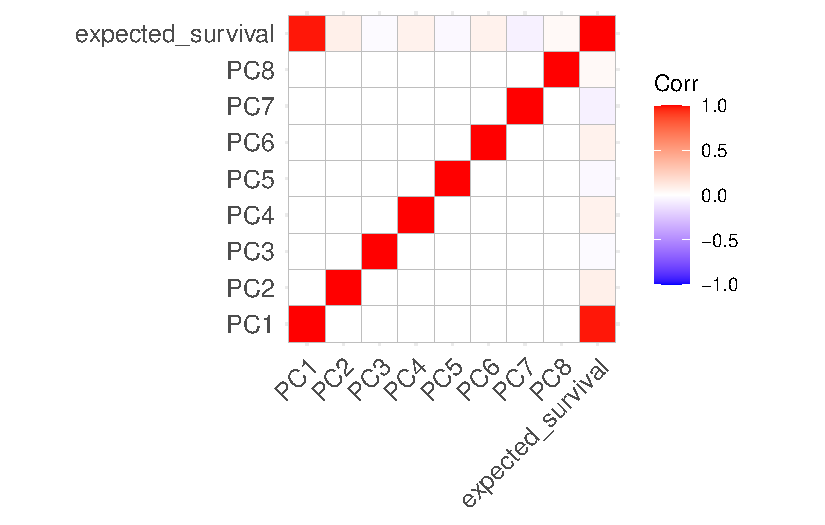
\includegraphics{analysis_files/figure-pdf/unnamed-chunk-30-1.pdf}

}

\end{figure}

\hypertarget{pca-2-principal-components}{%
\section{PCA: 2 Principal Components}\label{pca-2-principal-components}}

\begin{Shaded}
\begin{Highlighting}[]
\CommentTok{\# Create a subset with 2 principal components}
\NormalTok{significant\_pcs }\OtherTok{=} \FunctionTok{c}\NormalTok{(}\DecValTok{1}\NormalTok{,}\DecValTok{2}\NormalTok{,}\DecValTok{9}\NormalTok{)}
\NormalTok{train\_pca }\OtherTok{\textless{}{-}}\NormalTok{ training\_set[, significant\_pcs]}
\NormalTok{test\_pca }\OtherTok{\textless{}{-}}\NormalTok{ test\_set[, significant\_pcs]}
\end{Highlighting}
\end{Shaded}

\begin{Shaded}
\begin{Highlighting}[]
\CommentTok{\# reproducible random sampling}
\FunctionTok{set.seed}\NormalTok{(my\_seed)}

\CommentTok{\# Fit a multiple linear regression model}
\NormalTok{reg\_model }\OtherTok{\textless{}{-}} \FunctionTok{lm}\NormalTok{(expected\_survival }\SpecialCharTok{\textasciitilde{}}\NormalTok{ ., }
                \AttributeTok{data =}\NormalTok{ train\_pca)}

\CommentTok{\# Print a summary of the regression model}
\FunctionTok{tab\_model}\NormalTok{(reg\_model, }\AttributeTok{title =} \StringTok{"2 Principal Components Regression"}\NormalTok{,}
          \AttributeTok{string.p=}\StringTok{"P{-}value"}\NormalTok{, }\AttributeTok{string.stat =} \StringTok{"T{-}score"}\NormalTok{,}
          \AttributeTok{string.se =} \StringTok{"Std. Error"}\NormalTok{,}
          \AttributeTok{string.resp =} \StringTok{"Response"}\NormalTok{,}
          \AttributeTok{string.ci =} \StringTok{"Conf Int."}\NormalTok{,}
          \AttributeTok{show.se=}\NormalTok{T, }\AttributeTok{show.stat =}\NormalTok{ T,}
          \AttributeTok{CSS =} \FunctionTok{list}\NormalTok{(}
             \AttributeTok{css.depvarhead =} \StringTok{\textquotesingle{}font{-}weight: bold; text{-}align: left;\textquotesingle{}}\NormalTok{,}
             \AttributeTok{css.summary =} \StringTok{\textquotesingle{}color: \#10759B; font{-}weight: bold;\textquotesingle{}}
\NormalTok{           ))}
\end{Highlighting}
\end{Shaded}

\begin{longtable}[]{@{}cccccc@{}}
\caption{2 Principal Components Regression}\tabularnewline
\toprule\noalign{}
\endfirsthead
\endhead
\bottomrule\noalign{}
\endlastfoot
~ &
\multicolumn{5}{>{\centering\arraybackslash}p{(\columnwidth - 10\tabcolsep) * \real{0.0000} + 8\tabcolsep}@{}}{%
expected\_survival} \\
Predictors & Estimates & Std. Error & Conf Int. & T-score & P-value \\
(Intercept) & 97.05 & 3.58 & 89.78~--~104.32 & 27.07 &
\textbf{\textless0.001} \\
PC1 & 29.40 & 0.90 & 27.58~--~31.23 & 32.64 & \textbf{\textless0.001} \\
PC2 & 4.59 & 1.68 & 1.18~--~8.00 & 2.73 & \textbf{0.010} \\
Observations &
\multicolumn{5}{>{\raggedright\arraybackslash}p{(\columnwidth - 10\tabcolsep) * \real{0.0000} + 8\tabcolsep}@{}}{%
39} \\
R\textsuperscript{2} / R\textsuperscript{2} adjusted &
\multicolumn{5}{>{\raggedright\arraybackslash}p{(\columnwidth - 10\tabcolsep) * \real{0.0000} + 8\tabcolsep}@{}}{%
0.968 / 0.966} \\
\end{longtable}

\begin{Shaded}
\begin{Highlighting}[]
\CommentTok{\# Calculate PRESS}
\CommentTok{\# cat("PRESS: ", PRESS(reg\_model), "\textbackslash{}n")}
\NormalTok{PRESS\_2pc }\OtherTok{\textless{}{-}} \FunctionTok{PRESS}\NormalTok{(reg\_model)}

\CommentTok{\# Calculate predicted R\^{}2}
\CommentTok{\# cat("Predicted R\^{}2: ", pred\_r\_squared(reg\_model), "\textbackslash{}n")}
\NormalTok{R2\_2pc }\OtherTok{\textless{}{-}} \FunctionTok{pred\_r\_squared}\NormalTok{(reg\_model)}

\CommentTok{\# Print 2PC prediction results}
\NormalTok{predict\_2pc }\OtherTok{\textless{}{-}} \FunctionTok{cbind}\NormalTok{(PRESS\_2pc, R2\_2pc)}

\CommentTok{\# table format}
\FunctionTok{kbl}\NormalTok{(predict\_2pc, }\AttributeTok{caption =} \StringTok{"2 Principal Components Prediction Metrics"}\NormalTok{,}
    \AttributeTok{digits =} \DecValTok{4}\NormalTok{) }\SpecialCharTok{\%\textgreater{}\%}
  \FunctionTok{kable\_paper}\NormalTok{(}\StringTok{"hover"}\NormalTok{, }\AttributeTok{full\_width =}\NormalTok{ F)}
\end{Highlighting}
\end{Shaded}

\begin{table}

\caption{2 Principal Components Prediction Metrics}
\centering
\begin{tabular}[t]{r|r}
\hline
PRESS\_2pc & R2\_2pc\\
\hline
25699.6 & 0.9538\\
\hline
\end{tabular}
\end{table}

\hypertarget{principal-components-regression}{%
\subsection{\texorpdfstring{\textbf{Principal Components
Regression}}{Principal Components Regression}}\label{principal-components-regression}}

\begin{itemize}
\tightlist
\item
  PCA is used to calculate principal components that can then be used
  in~principal components regression. This type of regression is often
  used when~multicollinearity~exists between predictors in a data set.
\end{itemize}

\begin{Shaded}
\begin{Highlighting}[]
\CommentTok{\# reproducible random sampling}
\FunctionTok{set.seed}\NormalTok{(my\_seed)}

\NormalTok{y }\OtherTok{=}\NormalTok{ train\_pca}\SpecialCharTok{$}\NormalTok{expected\_survival}

\CommentTok{\# fit PCR}
\NormalTok{pcr\_model }\OtherTok{\textless{}{-}} \FunctionTok{pcr}\NormalTok{(y }\SpecialCharTok{\textasciitilde{}}\NormalTok{ PC1}\SpecialCharTok{+}\NormalTok{PC2, }\AttributeTok{data=}\NormalTok{train\_pca, }\AttributeTok{validation=}\StringTok{"CV"}\NormalTok{)}
\FunctionTok{print}\NormalTok{(pcr\_model)}
\end{Highlighting}
\end{Shaded}

\begin{verbatim}
Principal component regression, fitted with the singular value decomposition algorithm.
Cross-validated using 10 random segments.
Call:
pcr(formula = y ~ PC1 + PC2, data = train_pca, validation = "CV")
\end{verbatim}

\begin{Shaded}
\begin{Highlighting}[]
\CommentTok{\# table format}
\FunctionTok{kbl}\NormalTok{(pcr\_model}\SpecialCharTok{$}\NormalTok{residuals, }\AttributeTok{caption =} \StringTok{"PCA Residuals"}\NormalTok{,}
    \AttributeTok{digits =} \DecValTok{4}\NormalTok{) }\SpecialCharTok{\%\textgreater{}\%}
  \FunctionTok{kable\_paper}\NormalTok{(}\StringTok{"hover"}\NormalTok{, }\AttributeTok{full\_width =}\NormalTok{ F)}
\end{Highlighting}
\end{Shaded}

\begin{table}

\caption{PCA Residuals}
\centering
\begin{tabular}[t]{l|r|r}
\hline
  & y.1 comps & y.2 comps\\
\hline
1 & 0.1506 & -0.7094\\
\hline
2 & 14.8415 & 8.7438\\
\hline
3 & -9.9048 & -15.6499\\
\hline
4 & -11.9950 & -10.5934\\
\hline
5 & 14.5581 & 7.4172\\
\hline
6 & 10.5628 & -4.1105\\
\hline
7 & -1.1997 & -1.8621\\
\hline
8 & -13.8770 & -8.7908\\
\hline
10 & -10.6707 & -7.5478\\
\hline
13 & 15.9325 & -6.8066\\
\hline
14 & -28.4995 & -32.2191\\
\hline
15 & 13.7912 & 10.2807\\
\hline
19 & 2.2654 & -4.9708\\
\hline
20 & 20.7004 & 18.6124\\
\hline
22 & -22.7913 & -18.7054\\
\hline
24 & 0.3036 & -1.8158\\
\hline
27 & 15.1056 & 16.6785\\
\hline
29 & -18.5425 & -18.3174\\
\hline
30 & 7.9759 & -3.5721\\
\hline
31 & 61.8084 & 55.7883\\
\hline
32 & -20.9204 & -5.0790\\
\hline
33 & -12.8183 & -9.2901\\
\hline
34 & 1.6594 & -0.6758\\
\hline
35 & -17.3032 & -12.3010\\
\hline
36 & -17.2435 & -19.9354\\
\hline
37 & -4.2019 & -9.4719\\
\hline
38 & -90.8171 & -71.1562\\
\hline
39 & 57.1428 & 59.6527\\
\hline
41 & 10.0589 & 4.0816\\
\hline
42 & 18.5721 & 29.7334\\
\hline
44 & 3.2955 & -4.0228\\
\hline
45 & 8.2807 & 7.3105\\
\hline
46 & -17.5634 & -10.1654\\
\hline
49 & 14.4348 & 13.0494\\
\hline
50 & 5.5387 & 3.5868\\
\hline
51 & -9.4323 & 29.4206\\
\hline
54 & 10.5787 & 15.4795\\
\hline
55 & -1.1796 & 1.1198\\
\hline
56 & 1.4025 & -3.1866\\
\hline
\end{tabular}
\end{table}

\hypertarget{pca-cross-validation-model}{%
\subsection{PCA: Cross-Validation
Model}\label{pca-cross-validation-model}}

\begin{Shaded}
\begin{Highlighting}[]
\CommentTok{\# reproducible random sampling}
\FunctionTok{set.seed}\NormalTok{(my\_seed)}

\CommentTok{\# Cross{-}validation with n folds}
\NormalTok{k\_10 }\OtherTok{\textless{}{-}} \FunctionTok{trainControl}\NormalTok{(}\AttributeTok{method =} \StringTok{"cv"}\NormalTok{, }\AttributeTok{number =} \DecValTok{10}\NormalTok{)}

\CommentTok{\# training the model }
\NormalTok{model\_cv }\OtherTok{\textless{}{-}} \FunctionTok{train}\NormalTok{(expected\_survival }\SpecialCharTok{\textasciitilde{}}\NormalTok{ ., }
                  \AttributeTok{data =}\NormalTok{ train\_pca,}
                  \AttributeTok{method =} \StringTok{"lm"}\NormalTok{,}
                  \AttributeTok{trControl =}\NormalTok{ k\_10)}

\CommentTok{\# Print Model Performance}
\FunctionTok{print}\NormalTok{(model\_cv)}
\end{Highlighting}
\end{Shaded}

\begin{verbatim}
Linear Regression 

39 samples
 2 predictor

No pre-processing
Resampling: Cross-Validated (10 fold) 
Summary of sample sizes: 35, 35, 35, 35, 35, 35, ... 
Resampling results:

  RMSE     Rsquared   MAE     
  21.7825  0.9761582  16.14872

Tuning parameter 'intercept' was held constant at a value of TRUE
\end{verbatim}

\begin{Shaded}
\begin{Highlighting}[]
\CommentTok{\# Metrics}
\NormalTok{cv\_results }\OtherTok{=}\NormalTok{ model\_cv}\SpecialCharTok{$}\NormalTok{results}
\FunctionTok{kbl}\NormalTok{(cv\_results, }\AttributeTok{caption =} \StringTok{"PCA: Cross{-}Validation Metrics"}\NormalTok{,}
    \AttributeTok{digits =} \DecValTok{4}\NormalTok{) }\SpecialCharTok{\%\textgreater{}\%}
  \FunctionTok{kable\_paper}\NormalTok{(}\StringTok{"hover"}\NormalTok{, }\AttributeTok{full\_width =}\NormalTok{ F)}
\end{Highlighting}
\end{Shaded}

\begin{table}

\caption{PCA: Cross-Validation Metrics}
\centering
\begin{tabular}[t]{l|r|r|r|r|r|r}
\hline
intercept & RMSE & Rsquared & MAE & RMSESD & RsquaredSD & MAESD\\
\hline
TRUE & 21.7825 & 0.9762 & 16.1487 & 14.0372 & 0.0377 & 8.5694\\
\hline
\end{tabular}
\end{table}

\hypertarget{predictions}{%
\section{Predictions}\label{predictions}}

\begin{Shaded}
\begin{Highlighting}[]
\CommentTok{\# Find the index position of the target feature}
\NormalTok{pred\_target\_index }\OtherTok{\textless{}{-}} \FunctionTok{grep}\NormalTok{(target\_name, }
                     \FunctionTok{colnames}\NormalTok{(test\_pca))}
\CommentTok{\#cat("Target Feature Index =", pred\_target\_index)}

\CommentTok{\# Create Predicted Target Feature (y{-}test) }
\NormalTok{y\_test }\OtherTok{\textless{}{-}}\NormalTok{ test\_pca[pred\_target\_index]}
\end{Highlighting}
\end{Shaded}

\begin{Shaded}
\begin{Highlighting}[]
\CommentTok{\# Predictions using the Cross{-}Validation model}
\NormalTok{y\_pred }\OtherTok{=} \FunctionTok{predict}\NormalTok{(model\_cv, }\AttributeTok{newdata =}\NormalTok{ test\_pca[, }\SpecialCharTok{{-}}\NormalTok{pred\_target\_index])}
\end{Highlighting}
\end{Shaded}

\begin{Shaded}
\begin{Highlighting}[]
\CommentTok{\# Prediction Results from y\_predictions}
\NormalTok{y\_pred }\OtherTok{\textless{}{-}} \FunctionTok{round}\NormalTok{(y\_pred, }\AttributeTok{digits =} \DecValTok{0}\NormalTok{)}
\end{Highlighting}
\end{Shaded}

\begin{Shaded}
\begin{Highlighting}[]
\CommentTok{\# Transform y\_test from data frame to numeric}
\NormalTok{y\_test }\OtherTok{\textless{}{-}} \FunctionTok{as.numeric}\NormalTok{(}\FunctionTok{unlist}\NormalTok{(y\_test))}

\NormalTok{prediction\_comparison }\OtherTok{\textless{}{-}} \FunctionTok{cbind}\NormalTok{(y\_pred, y\_test)}
\CommentTok{\# table format}
\FunctionTok{kbl}\NormalTok{(prediction\_comparison) }\SpecialCharTok{\%\textgreater{}\%}
  \FunctionTok{kable\_paper}\NormalTok{(}\StringTok{"hover"}\NormalTok{, }\AttributeTok{full\_width =}\NormalTok{ F)}
\end{Highlighting}
\end{Shaded}

\begin{table}
\centering
\begin{tabular}[t]{l|r|r}
\hline
  & y\_pred & y\_test\\
\hline
9 & 35 & 16\\
\hline
11 & 520 & 442\\
\hline
12 & 310 & 318\\
\hline
16 & 26 & 25\\
\hline
17 & 298 & 284\\
\hline
18 & 125 & 152\\
\hline
21 & 159 & 160\\
\hline
23 & 149 & 141\\
\hline
25 & 191 & 197\\
\hline
26 & 81 & 95\\
\hline
28 & 2 & 2\\
\hline
40 & 86 & 78\\
\hline
43 & 113 & 38\\
\hline
47 & 182 & 171\\
\hline
48 & 585 & 657\\
\hline
52 & 33 & 7\\
\hline
53 & 88 & 92\\
\hline
\end{tabular}
\end{table}

\hypertarget{prediction-metrics}{%
\subsection{Prediction Metrics}\label{prediction-metrics}}

\begin{Shaded}
\begin{Highlighting}[]
\CommentTok{\# Calculate Mean Absolute Error (MAE)}
\NormalTok{MAE\_value }\OtherTok{\textless{}{-}} \FunctionTok{mae}\NormalTok{(y\_pred, y\_test)}
\CommentTok{\#cat("MAE =", mae\_value)}

\CommentTok{\# Calculate MSE}
\NormalTok{MSE\_predict }\OtherTok{\textless{}{-}} \FunctionTok{mean}\NormalTok{((y\_pred }\SpecialCharTok{{-}}\NormalTok{ y\_test)}\SpecialCharTok{\^{}}\DecValTok{2}\NormalTok{)}
\CommentTok{\#cat("\textbackslash{}nMSE =", mse\_predict)}

\CommentTok{\# Calculate RMSE}
\NormalTok{RMSE\_predict }\OtherTok{\textless{}{-}} \FunctionTok{sqrt}\NormalTok{(}\FunctionTok{mean}\NormalTok{((y\_pred }\SpecialCharTok{{-}}\NormalTok{ y\_test)}\SpecialCharTok{\^{}}\DecValTok{2}\NormalTok{))}
\CommentTok{\#cat("\textbackslash{}nRMSE =", rmse\_predict)}

\CommentTok{\# Calculate R{-}squared (R\^{}2)}
\NormalTok{predicted\_R2 }\OtherTok{\textless{}{-}} \DecValTok{1} \SpecialCharTok{{-}} \FunctionTok{sum}\NormalTok{((y\_test }\SpecialCharTok{{-}}\NormalTok{ y\_pred)}\SpecialCharTok{\^{}}\DecValTok{2}\NormalTok{) }\SpecialCharTok{/} 
  \FunctionTok{sum}\NormalTok{((y\_test }\SpecialCharTok{{-}} \FunctionTok{mean}\NormalTok{(y\_test))}\SpecialCharTok{\^{}}\DecValTok{2}\NormalTok{)}
\CommentTok{\# cat("\textbackslash{}nPredicted R\^{}2 =", predicted\_r2)}

\NormalTok{prediction\_metrics\_df }\OtherTok{\textless{}{-}} \FunctionTok{cbind}\NormalTok{(MAE\_value, MSE\_predict,}
\NormalTok{                               RMSE\_predict, predicted\_R2)}
\CommentTok{\# table format}
\FunctionTok{kbl}\NormalTok{(prediction\_metrics\_df, }\AttributeTok{digits =} \DecValTok{4}\NormalTok{) }\SpecialCharTok{\%\textgreater{}\%}
  \FunctionTok{kable\_paper}\NormalTok{(}\StringTok{"hover"}\NormalTok{, }\AttributeTok{full\_width =}\NormalTok{ F)}
\end{Highlighting}
\end{Shaded}

\begin{table}
\centering
\begin{tabular}[t]{r|r|r|r}
\hline
MAE\_value & MSE\_predict & RMSE\_predict & predicted\_R2\\
\hline
21.8824 & 1142.235 & 33.797 & 0.96\\
\hline
\end{tabular}
\end{table}

\hypertarget{training-conclusion}{%
\section{Training Conclusion}\label{training-conclusion}}

In conclusion, this project has demonstrated the effectiveness of
Principal Component Analysis (PCA) in dimension reduction with the
following key points:

\begin{itemize}
\item
  PCA was able to reduce from 37 features down to just 2 principal
  components.
\item
  The best score of R\^{}2 = 97.61\% was from the Linear Regression with
  Cross-validation model.
\item
  The predicted R\^{}2 = 96\%
\item
  The average deviation between the predicted values, and observed
  values for `Expected Survival' is RMSE = 33.8.
\item
  The model has not been exposed to unseen data with a large amount of
  observations to asses its robustness, and reliability.
\end{itemize}

\bookmarksetup{startatroot}

\hypertarget{results-2}{%
\chapter{Results}\label{results-2}}

The Dialysis dataset consists of 55 observations of 39 variables with 1
discrete variable (States/Territories) and 38 continuous variables. For
the principal component analysis, 37 of the 38 continuous variables were
used; the variable expected\_survival was excluded from PCA in order to
use it as a target for model building in the latter part of the
analysis.

Principal component analysis was performed using a singular value
decomposition approach. Among the resulting principal components, the
first PC captures 40.80\% of the variance in the data, and the first two
principal components capture 50.27\% of the variance. The first four PCs
capture 67.66\% of the variance, or just over two-thirds; after the
fourth PC, the variance captured by each successive PC begins to
diminish relative to PCs one through four. The first ten PCs capture
88.67\% of the variance, and in terms of dimensionality reduction over
90\% of the information in the dataset can be explained by only 11 PCs
when compared to the original 38 continuous variables.

The variables which contribute the most to PC1 are
expected\_hospital\_readmission, expected\_transfusion, and
expected\_hospitalization, although the percent of total contribution to
PC1 by any one variable is not outsized relative to the remaining
variables. PC2, which is orthogonal to PC1, has relatively large
contributions from the five variables measuring levels of phosphorus;
patterns or trends in the data such as these can be further explored
using other methodologies after being highlighted in PCA {[}26{]}.

From here, the analysis extends PCA via model building using linear
regression with a technique known as principal component regression,
with expected\_survival used as the response variable. The data is first
split into training and testing sets; then the data is centered and
scaled, after which PCA is applied to each set. The first model is
created for illustrative purposes, using 8 principle components from the
training set of 39 observations. The estimates and significance of each
PC regressor demonstrates the differences between variance captured from
the data and usefulness in a linear model; for example, PC4 is a
significant regressor despite capturing less variance than PC3 in the
training data.

The analysis concludes by building and comparing two linear regression
models using the first two prinicipal components. The first model is a
straightforward linear model using the lm() function from the stats
package in R {[}27{]}. The second model uses 10-fold cross-validation
for a linear model using the train() and trainControl() functions from
the caret package in R {[}28{]}. Both models produce an \(R^2\) above
96\% and a predicted \(R^2\) above 95\% with a 1\% advantage on the
cross-validation model. Although the interpretations of the regressors
for these PCA models is different than those of a linear regression on
the original variables, the lower dimensionality of the data may be
desirable as a more simple model which still captures a large portion of
the variance in the original data.

\bookmarksetup{startatroot}

\hypertarget{discussion}{%
\chapter{Discussion}\label{discussion}}

Principal Component Analysis (PCA) is a foundational multivariate
analysis technique that has been widely employed to extract essential
information from intricate multivariate datasets and effectively reduce
dimensionality. Due to its simplicity and versatility, PCA has become
one of the widely adopted tools for understanding and exploring data
features in a multivariate dataset. This approach leverages singular
value decomposition to restructure datasets and facilitates subsequent
statistical analysis. By doing so, PCA simplifies complexity,
eliminating superfluous details and redundant information arising from
the original dataset. The outcome is a set of principal components that
capture most of the variance explaining the original variables. To
accomplish this, PCA first converts the dataset into a covariance matrix
and then employs singular value decomposition to identify eigenvalues
and eigenvectors, representing the loadings of the newly generated
principal components. These components can typically account for over
70-80\% of the original variables' variances.

PCA's importance in data analysis is underscored by its adaptability to
various scenarios and data types, including binary, ordinal,
compositional, and discrete data. Moreover, the PCA algorithm has proven
effective in reducing the dimensions of vast datasets with high
accuracy, significantly improving classification tasks. It plays a
crucial role in exploratory data analysis and preliminary data
processing, acting as a feature extraction and dimensionality reduction
tool. One of its main benefits is its ability to mitigate
multicollinearity issues, which can otherwise lead to biased results in
statistical analyses.

Despite its numerous advantages, PCA does come with certain limitations.
For instance, it is sensitive to the presence of outliers, which can
distort the results and compromise its effectiveness. Furthermore, the
new features or components generated through PCA are not readily
interpretable, making it challenging to explain their meaning in a
straightforward manner. Nonetheless, PCA remains a pivotal technique in
data analysis, offering a powerful means to navigate complex datasets
and uncover their underlying structures.

\bookmarksetup{startatroot}

\hypertarget{references}{%
\chapter{References}\label{references}}

\hypertarget{refs}{}
\begin{CSLReferences}{0}{0}
\leavevmode\vadjust pre{\hypertarget{ref-ringner2008principal}{}}%
\CSLLeftMargin{{[}1{]} }%
\CSLRightInline{M. Ringnér, {``What is principal component analysis?''}
\emph{Nature biotechnology}, vol. 26, no. 3, pp. 303--304, 2008.}

\leavevmode\vadjust pre{\hypertarget{ref-jolliffe2016principal}{}}%
\CSLLeftMargin{{[}2{]} }%
\CSLRightInline{I. T. Jolliffe and J. Cadima, {``Principal component
analysis: A review and recent developments,''} \emph{Philosophical
transactions of the royal society A: Mathematical, Physical and
Engineering Sciences}, vol. 374, no. 2065, p. 20150202, 2016.}

\leavevmode\vadjust pre{\hypertarget{ref-esposito2020introducing}{}}%
\CSLLeftMargin{{[}3{]} }%
\CSLRightInline{D. Esposito and F. Esposito, \emph{Introducing machine
learning}. Microsoft Press, 2020.}

\leavevmode\vadjust pre{\hypertarget{ref-hasan2021review}{}}%
\CSLLeftMargin{{[}4{]} }%
\CSLRightInline{B. M. S. Hasan and A. M. Abdulazeez, {``A review of
principal component analysis algorithm for dimensionality reduction,''}
\emph{Journal of Soft Computing and Data Mining}, vol. 2, no. 1, pp.
20--30, 2021.}

\leavevmode\vadjust pre{\hypertarget{ref-pearson1901liii}{}}%
\CSLLeftMargin{{[}5{]} }%
\CSLRightInline{K. Pearson, {``LIII. On lines and planes of closest fit
to systems of points in space,''} \emph{The London, Edinburgh, and
Dublin philosophical magazine and journal of science}, vol. 2, no. 11,
pp. 559--572, 1901.}

\leavevmode\vadjust pre{\hypertarget{ref-hotelling1933analysis}{}}%
\CSLLeftMargin{{[}6{]} }%
\CSLRightInline{H. Hotelling, {``Analysis of a complex of statistical
variables into principal components.''} \emph{Journal of educational
psychology}, vol. 24, no. 6, p. 417, 1933.}

\leavevmode\vadjust pre{\hypertarget{ref-fisher1923studies}{}}%
\CSLLeftMargin{{[}7{]} }%
\CSLRightInline{R. A. Fisher and W. A. Mackenzie, {``Studies in crop
variation. II. The manurial response of different potato varieties,''}
\emph{The Journal of Agricultural Science}, vol. 13, no. 3, pp.
311--320, 1923.}

\leavevmode\vadjust pre{\hypertarget{ref-greenacre2022principal}{}}%
\CSLLeftMargin{{[}8{]} }%
\CSLRightInline{M. Greenacre, P. J. Groenen, T. Hastie, A. I. d'Enza, A.
Markos, and E. Tuzhilina, {``Principal component analysis,''}
\emph{Nature Reviews Methods Primers}, vol. 2, no. 1, p. 100, 2022.}

\leavevmode\vadjust pre{\hypertarget{ref-everitt2011introduction}{}}%
\CSLLeftMargin{{[}9{]} }%
\CSLRightInline{B. Everitt and T. Hothorn, \emph{An introduction to
applied multivariate analysis with r}. Springer Science \& Business
Media, 2011.}

\leavevmode\vadjust pre{\hypertarget{ref-abdi2010principal}{}}%
\CSLLeftMargin{{[}10{]} }%
\CSLRightInline{H. Abdi and L. J. Williams, {``Principal component
analysis,''} \emph{WIREs Computational Statistics}, vol. 2, no. 4, pp.
433--459, 2010, doi: \url{https://doi.org/10.1002/wics.101}. Available:
\url{https://wires.onlinelibrary.wiley.com/doi/abs/10.1002/wics.101}}

\leavevmode\vadjust pre{\hypertarget{ref-lever2017points}{}}%
\CSLLeftMargin{{[}11{]} }%
\CSLRightInline{J. Lever, M. Krzywinski, and N. Altman, {``Points of
significance: Principal component analysis,''} \emph{Nature methods},
vol. 14, no. 7, pp. 641--643, 2017.}

\leavevmode\vadjust pre{\hypertarget{ref-maindonald2006data}{}}%
\CSLLeftMargin{{[}12{]} }%
\CSLRightInline{J. Maindonald and J. Braun, \emph{Data analysis and
graphics using r: An example-based approach}, vol. 10. Cambridge
University Press, 2006.}

\leavevmode\vadjust pre{\hypertarget{ref-gewers2021principal}{}}%
\CSLLeftMargin{{[}13{]} }%
\CSLRightInline{F. L. Gewers \emph{et al.}, {``Principal component
analysis: A natural approach to data exploration,''} \emph{ACM Computing
Surveys (CSUR)}, vol. 54, no. 4, pp. 1--34, 2021.}

\leavevmode\vadjust pre{\hypertarget{ref-pedregosa2011scikit}{}}%
\CSLLeftMargin{{[}14{]} }%
\CSLRightInline{F. Pedregosa \emph{et al.}, {``Scikit-learn: Machine
learning in python,''} \emph{the Journal of machine Learning research},
vol. 12, pp. 2825--2830, 2011.}

\leavevmode\vadjust pre{\hypertarget{ref-turk1991eigenfaces}{}}%
\CSLLeftMargin{{[}15{]} }%
\CSLRightInline{M. Turk and A. Pentland, {``Eigenfaces for
recognition,''} \emph{Journal of cognitive neuroscience}, vol. 3, no. 1,
pp. 71--86, 1991.}

\leavevmode\vadjust pre{\hypertarget{ref-zhang2008eigenfaces}{}}%
\CSLLeftMargin{{[}16{]} }%
\CSLRightInline{S. Zhang and M. Turk, {``Eigenfaces,''}
\emph{Scholarpedia}, vol. 3, no. 9, p. 4244, 2008.}

\leavevmode\vadjust pre{\hypertarget{ref-prcomp2023ref}{}}%
\CSLLeftMargin{{[}17{]} }%
\CSLRightInline{R Core Team, {``Prcomp, a function of r: A language and
environment for statistical computing.''} R Foundation for Statistical
Computing, Vienna, Austria, 2023. Available:
\url{https://www.rdocumentation.org/packages/stats/versions/3.6.2/topics/prcomp}.
{[}Accessed: Oct. 16, 2023{]}}

\leavevmode\vadjust pre{\hypertarget{ref-bennett2021linear}{}}%
\CSLLeftMargin{{[}18{]} }%
\CSLRightInline{S. R. Bennett, {``Linear algebra for data science.''}
2021. Available:
\url{https://shainarace.github.io/LinearAlgebra/index.html}.
{[}Accessed: Oct. 16, 2023{]}}

\leavevmode\vadjust pre{\hypertarget{ref-hopcroft2014foundations}{}}%
\CSLLeftMargin{{[}19{]} }%
\CSLRightInline{J. Hopcroft and R. Kannan, \emph{Foundations of data
science}. 2014.}

\leavevmode\vadjust pre{\hypertarget{ref-luenberger1997optimization}{}}%
\CSLLeftMargin{{[}20{]} }%
\CSLRightInline{D. G. Luenberger, \emph{Optimization by vector space
methods}. John Wiley \& Sons, 1997.}

\leavevmode\vadjust pre{\hypertarget{ref-eduflair2020}{}}%
\CSLLeftMargin{{[}21{]} }%
\CSLRightInline{E. K. CS, {``PCA problem / how to compute principal
components / KTU machine learning.''} YouTube, 2020. Available:
\url{https://youtu.be/MLaJbA82nzk}. {[}Accessed: Nov. 01, 2023{]}}

\leavevmode\vadjust pre{\hypertarget{ref-misc_abalone_1}{}}%
\CSLLeftMargin{{[}22{]} }%
\CSLRightInline{S. Nash Warwick and W. Ford, {``{Abalone}.''} UCI
Machine Learning Repository, 1995.}

\leavevmode\vadjust pre{\hypertarget{ref-pages2014multiple}{}}%
\CSLLeftMargin{{[}23{]} }%
\CSLRightInline{J. Pagès, \emph{Multiple factor analysis by example
using r}. CRC Press, 2014.}

\leavevmode\vadjust pre{\hypertarget{ref-dialysis2023july}{}}%
\CSLLeftMargin{{[}24{]} }%
\CSLRightInline{{``Quarterly dialysis facility care compare (QDFCC)
report: July 2023.''} Centers for Medicare \& Medicaid Services (CMS).
Available: \url{https://data.cms.gov/provider-data/dataset/2fpu-cgbb}.
{[}Accessed: Oct. 11, 2023{]}}

\leavevmode\vadjust pre{\hypertarget{ref-chumney2012pcaefa}{}}%
\CSLLeftMargin{{[}25{]} }%
\CSLRightInline{F. Chumney, {``PCA, EFA, CFA,''} pp. 2--3, 6, Sep.,
2012, Available:
\url{https://www.westga.edu/academics/research/vrc/assets/docs/PCA-EFA-CFA_EssayChumney_09282012.pdf}}

\leavevmode\vadjust pre{\hypertarget{ref-bro2014principal}{}}%
\CSLLeftMargin{{[}26{]} }%
\CSLRightInline{R. Bro and A. K. Smilde, {``Principal component
analysis,''} \emph{Analytical methods}, vol. 6, no. 9, pp. 2812--2831,
2014.}

\leavevmode\vadjust pre{\hypertarget{ref-lm2023ref}{}}%
\CSLLeftMargin{{[}27{]} }%
\CSLRightInline{R Core Team, {``Lm: Fitting linear models.''} R
Foundation for Statistical Computing, Vienna, Austria, 2023. Available:
\url{https://www.rdocumentation.org/packages/stats/versions/3.6.2/topics/lm}.
{[}Accessed: Nov. 08, 2023{]}}

\leavevmode\vadjust pre{\hypertarget{ref-caret2023ref}{}}%
\CSLLeftMargin{{[}28{]} }%
\CSLRightInline{Kuhn and Max, {``Building predictive models in r using
the caret package,''} \emph{Journal of Statistical Software}, vol. 28,
no. 5, pp. 1--26, 2008, doi:
\href{https://doi.org/10.18637/jss.v028.i05}{10.18637/jss.v028.i05}.
Available:
\url{https://www.jstatsoft.org/index.php/jss/article/view/v028i05}}

\end{CSLReferences}

\bookmarksetup{startatroot}

\hypertarget{presentation}{%
\chapter*{Presentation}\label{presentation}}
\addcontentsline{toc}{chapter}{Presentation}

\markboth{Presentation}{Presentation}



\end{document}
